\documentclass[fontsize=12pt, twoside, a4paper]{scrreprt} % koma class

% paper properties
\usepackage{geometry}
\geometry{left=3.5cm, right=2.0cm, top=2.5cm, bottom=2.5cm}

% charset and language
\usepackage[T1]{fontenc} % charset
\usepackage[utf8]{inputenc} % charset
\usepackage[german, polish, english]{babel} % language
\let\babellll\lll % fix for \lll already defined by babel
\let\lll\relax
\babeltags{de=german}
\babeltags{po=polish}

% text formatting
\usepackage{url}
\usepackage{lipsum}
\usepackage{mathptmx} % times new roman
\usepackage[onehalfspacing]{setspace}
\AfterTOCHead{\singlespacing}
\KOMAoptions{
	parskip=half,
	titlepage=true,
	draft=true  %TODO false in print
	}
\addtokomafont{disposition}{\normalfont}
\addtokomafont{caption}{\footnotesize}
\setkomafont{captionlabel}{\bfseries}
\usepackage{color}

% special symbols
\usepackage{soul}
\usepackage{amsmath}
\usepackage{amssymb}
\let\mathlll\lll % fix for \lll already defined by babel reassign to \mathlll
\let\lll\babellll
\usepackage{amstext}
\usepackage{chemarr}
\usepackage{textcomp}

% lists
\usepackage{acronym}
\usepackage{natbib}
\setcitestyle{sort,authoryear,square,semicolon,aysep={}}
\renewcommand{\bibfont}{\small \singlespacing}
\KOMAoptions{
	toc=listof,
	toc=bibliography,
	listof=flat,
	}

% tables
\KOMAoption{captions}{tableheading}
\usepackage{multirow}
\usepackage{multicol}
\usepackage{array}
\usepackage{longtable}

% images
\usepackage{graphicx}

% fix hbox warn for bbl
\usepackage{etoolbox}
\apptocmd{\thebibliography}{\raggedright}{}{}

% hyperlinks
\usepackage[hidelinks, colorlinks=false, urlcolor=blue, linkcolor=blue, citecolor = blue]{hyperref}
\hypersetup{pdftitle={A comprehensive study on deforestation in the tropical zone}}
\hypersetup{pdfauthor={Tobias Seydewitz}}
\hypersetup{pdfsubject={Evaluating the direct deforestation drivers, estimating the carbon emissions trough deforestation and evaluating the ecosystem service value balance of land cover change in the tropical zone between 23.43N and 23.43S.}}
\hypersetup{pdfcreator={Tobias Seydewitz}}
\hypersetup{pdfproducer={Tobias Seydewitz}}
\hypersetup{pdfkeywords={climate, emissions, soil organic carbon change, GIS, ecosystem service values, deforestation}}
\hypersetup{pdfdisplaydoctitle=true}

% new commands
\newcommand*\BlankPage{\newpage\null\thispagestyle{empty}\newpage}
\newcommand{\leadingzero}[1]{\ifnum #1<10 0\the#1\else\the#1\fi}
\newcommand{\todayI}{\leadingzero{\day}.\leadingzero{\month}.\the\year}
\newcommand{\STAB}[1]{\begin{tabular}{@{}c@{}}#1\end{tabular}}
\newcommand*\note[1]{{\color{red} #1}}
\renewcommand*{\captionformat}{.\ }

%\recalctypearea

%\usepackage{tabularx}
%\usepackage{caption}
%\usepackage{rotating}
%\usepackage{tcolorbox} 
%\usepackage{color}
%\usepackage{colortbl}
%\usepackage{color}
%\usepackage{float}

%\tiny 6pt
%\scriptsize 8pt
%\footnotesize 10pt
%\small 10.95pt
%\normalsize 12pt
%\large 14.4pt
%\Large 17.28pt
%\LARGE 20.7pt
%\huge 24.88pt
%\Huge 24.88pt

\begin{document}
	%\nocite{*} % cite all no matter if used in text
	\bibliographystyle{tobinat}

	\hypersetup{pageanchor=false}

		% title page
		\begin{titlepage}
	\begin{singlespace}
		\begin{center}
			\Large{Warsaw University of Life Sciences WULS – SGGW}\\
			\Large{in Warsaw}\\
			\Large{Faculty of Forestry}

			\smallskip

			\Large{Eberswalde University for Sustainable Development – HNEE}\\
			\Large{University of Applied Sciences}\\
			\Large{Faculty of Forest and Environment}

			\bigskip

			\large{Tobias Seydewitz}\\
			\normalsize{Album number SGGW: 178311}\\
			\normalsize{Album number HNEE: 15210024}

			\vspace{2cm}
 
			 \huge{Globalna ocena czynników powodujących wylesianie w tropikach: wpływ na zasoby węgla i usługi ekosystemowe}

			 \Large{Global assessment of deforestation drivers across the tropics: impacts on carbon stocks and ecosystem services}

			\bigskip

			\large{Master's Thesis}\\
			\large{on the course of - Forestry}

			\vspace{2cm}

			\begin{flushright}
				\normalsize{Thesis written under the supervision of}\\
				\normalsize{Dr. Prajal Pradhan}\\
				\normalsize{Potsdam Institute of Climate Impact Research}\\
				\normalsize{Research Domain II - Climate Climate Impacts \& Vulnerabilities}
			\end{flushright}

			\bigskip

			\normalsize{Potsdam, \the\year}
		\end{center}
	\end{singlespace}
\end{titlepage}
	\BlankPage

		% declarations
%		\thispagestyle{empty}

\begin{singlespace}
	\begin{po}
		\begin{center}
			\textbf{Oświadczenie promotora pracy}
		\end{center}
		Oświadczam, że niniejsza praca została przygotowana pod moim kierunkiem i stwierdzam, że spełnia warunki do przedstawienia tej pracy w postępowaniu o nadanie tytułu zawodowego.
	\end{po}
	\begin{center}
		\textbf{Declaration of the promoter}
	\end{center}
	I declare that this thesis was prepared under my supervision and I state that it meets the conditions for presenting such a body of work in the process of obtaining a professional title.
	\begin{de}
		\begin{center}
			\textbf{Erklärung des Betreuers}
		\end{center}
		Hiermit erkläre ich, dass die vorliegende Arbeit, unter meiner Leitung erstellt wurde und ich bestätige, dass sie die Bedingungen zur Verleihung des Abschlussdiploms erfüllt.
	\end{de}

	\vspace{2cm}

	\begin{tabular}{llll}
		Data & \makebox[3.9cm]{\dotfill} & Podpis promotora pracy & \makebox[3.9cm]{\dotfill}\\
		Date & & Signature of the promoter & \\
		Datum & & Unterschrift des Betreuers & \\
	\end{tabular}
\end{singlespace}
%	\BlankPage
%		\thispagestyle{empty}

\begin{singlespace}
	\begin{po}
		\begin{center}
			\textbf{Oświadczenie autora pracy}
		\end{center}
		Świadom odpowiedzialności prawnej, w tym odpowiedzialności karnej za złożenie fałszywego oświadczenia, oświadczam, że niniejsza praca dyplomowa została napisana przeze mnie samodzielnie i nie zawiera treści uzyskanych w sposób niezgodny z obowiązującymi przepisami prawa, w szczególności ustawą z dnia 4 lutego 1994 r.o prawie autorskim i prawach pokrewnych (Dz. U. Nr 90 poz. 631 z późn. zm.).
		
		Oświadczam, że przedstawiona praca nie była wcześniej podstawą żadnej procedury związanej z nadaniem dyplomu lub uzyskaniem tytułu zawodowego test. Lorem ipsum dolores anno sacntum
		
		Oświadczam, że niniejsza wersja pracy jest identyczna z załączoną wersją elektroniczną. Przyjmuję do wiadomości, że praca dyplomowa poddana zostanie procedurze antyplagiatowej.
	\end{po}
	\begin{center}
		\textbf{Declaration of the author}
	\end{center}
	Aware of the legal liability, including criminal liability for submitting a false statement, I
	declare that this thesis was written by myself alone and does not contain content obtained in
	a manner breaking applicable laws, in particular the Act of February 4, 1994 on copyright
	and related rights (Journal of Laws, no. 90, item 631, as amended).
	
	I certify that the work has not previously been the basis for any procedure in connection with
	obtaining a diploma or professional title.
	
	I declare that this version of the work is identical with the attached electronic version.
	
	I acknowledge that the thesis is subject to anti-plagiarism procedures.
	\begin{de}
		\begin{center}
			\textbf{Erklärung des Autors}
		\end{center}
		Gesetzlicher Haftpflicht, besonders der strafrechtlichen Verantwortlichkeit für Abgabe der falschen Erklärung bewusst, erkläre ich hiermit, dass vorliegende Diplomarbeit selbständig angefertigt wurde und keinen Inhalt enthält, der widerrechtlich erworben wurde, insbesondere nicht mit dem Gesetz über Urheberrecht vom 4. Februar 1994 (GB. Nr. 90, Pos. 631 mit späteren Änderungen) übereinstimmend.
		
		Ich erkläre auch, dass die Arbeit bisher keiner anderen Prüfungsbehörde vorgelegt wurde.
		
		Der Durchführung einer elektronischen Plagiatsprüfung stimme ich hiermit zu. Die eingereichte elektronische Fassung der Arbeit entspricht der eingereichten schriftlichen Fassung exakt.
	\end{de}

	\vspace{2cm}

	\begin{tabular}{llll}
		Data & \makebox[3.9cm]{\dotfill} & Podpis autora pracy & \makebox[3.9cm]{\dotfill}\\
		Date & & Signature of the author & \\
		Datum & & Unterschrift des Autors & \\
	\end{tabular}
\end{singlespace}

%	\BlankPage

%	\BlankPage
%	\BlankPage

		% abstracts
%		\thispagestyle{empty}

\begin{po}
	\begin{center}
		\textbf{Streszczenie}
	\end{center}
	\textbf{Tytuł: Text}
	
	Text
	
	Słowa kluczowe: Text
\end{po}
%	\BlankPage
%		\thispagestyle{empty}

\begin{center}
	\textbf{Summary}
\end{center}
\textbf{Title: Tropical deforestation and its impact on land cover, carbon losses, and ecosystem service values}

\begin{itemize}
	\item This study analyzes spatial explicitly the magnitudes of proximate deforestation driver, the related carbon losses by removal of biomass and soil organic carbon changes, and the ecosystem service value dynamics of tropical forest cover loss between 2001 and 2010.
	\item By applying the most recent global land cover datasets GlobeLand30 and Global Forest Change we quantified the proximate deforestation driver.
	\item We harmonized the datasets by applying the jaccard index.
	\item Two biomass maps are used to derive the carbon losses.
	\item To assess deforestation impacts on the ecosystem service dynamics the unit values from the three most common datasets are used.
	\item The harmonization revealed that tree cover agreement between both land cover is at its maximum within the canopy density interval $(10,100]$, while continental agreement differs in its interval.
	\item On global scale agriculture (79.7\%) is the most dominant deforestation driver, while the expansion of pastures contributed most (33.1\%).
	\item The continental scaled analysis revealed that proximate driver dynamics differ.
	\item In Latin America and Africa the expansion of pastures is the major driver, while Asia/Australia is dominated by regrowth dynamics.
	\item On the global scale 
\end{itemize}

Keywords: deforestation drivers, carbon losses, ecosystem service values, tropical zone, hexagon, Jaccard Index
%	\BlankPage
%		\thispagestyle{empty}

\begin{de}
	\begin{center}
		\textbf{Zusammenfassung}
	\end{center}
	\textbf{Titel: Quantifizierung der Triebkräft der tropischen Entwaldung und ihre Auswirkung auf die Kohlenstoffvorräte sowie Ökosystemdienstleistungen}

	In den Tropen ist Entwaldung einer der Hauptursachen für die Veränderung der Bodenbedeckung. Das kann auf verschiedene Ursachen zurückgeführt werden, die als direkte Triebkräfte der Entwaldung bezeichnet werden. Weltweit ist die fortschreitende Entwaldung eine Quelle für anthropogene Treibhausgas-Emissionen (THG) und trägt somit zum Klimawandel bei. Außerdem werden globale und kontinentale Ökosytemdiestleistungen in ihrer Funktionsweise durch Veränderungen der Waldstruktur gestört. Die räumliche Auswertung von Entwaldungstriebkräften ist aufwending und bestehende Datensätze sind nur eingeschränkt in niedriger Auflösung verfügbar. Weiterhin wurden THG-Emissionen nur für Biomasseverluste quantifiziert, während Kohlenstoffverluste durch Veränderungen des Bodengefüges nicht bewertet wurden. Schlußendlich wurde bisher nur der Bruttoverlust von Ökosystemdienstleistungen qunatifiziert ohne die Nettoverluste mit einzubeziehen. Ziel dieser Studie ist es die folgenden Dynamiken für den Zeitraum 2001-2010 zu analysieren: (1) die räumliche und quantitative Verteilung von Entwaldungstriebkräften, (2) die damit verbundenen Kohlenstoffverluste durch Biomasseverluste und Veränderung des Bodengefüges (3) die Wertentwicklung der Ökosystemdienstleistungen im globalem, kontinentalem, und regionalem Maßstab. Durch Aggregation der hochauflösenden Fernerkundungsdatensätze GlobeLand30 und Global Forest Change haben wir die Triebkräfte der Entwaldung quantifiziert. Die Bilanzierung der Kohlenstoffverluste durch die Entfernung von Biomasse erfolgte über einen Biomassedichtedatensatz. Um die Kohlenstoffverluste durch Veränderungen des Bodengefüges zu bestimmen haben wir die Koeffizienten von \citet{Don2010} verwendet. Die Bilanz der Ökosystemdienstleistungen wurde mit hilfe der drei gängisten Koeffizienten Datensätze erstellt. In den Tropen ist Landwirtschaft (79.7\%) der Hauptgrund für Entwaldung, während Expansion von Weideflächen (33.1\%) den größten Anteil daran hat. Weiterhin konnten wir feststellen das der Gesamtverlust von Kohlenstoff durch Entfernung von Biomasse 6757 Mt C beträgt, während der Kohlenstoffverlust durch Veränderung des Bodengefüges 583 ($\pm$ 105) Mt C beträgt. Der Bruttorverlust an Ökosystemdienstleistungen durch Entwaldung beträgt 414.1 Milliarden Dollar, während der Nettoverlust bei 63.1 Milliarden Dollar pro Jahr liegt. Unsere Ergebnisse zeigen das die bereits verfügbaren fernerkundungsdatensätze geeignet sind um Entwalungsdynamiken zu beschreiben sowie die Kohlenstoffverluste und Ökosystemdienstleistungen zu quantifizieren. Unsere studie zeigt das direkte Entwaldungstriebkräfte einen wesentlichen Beitrag zu den globalen Emissionen und dem Werteverlust in Ökosystemdienstleistungen beitragen.

	Schlüsselwörter: Entwaldung, direkte Triebkräfte, THG Emissionen, Ökosystemdienstleistungen, Tropen
\end{de}
%	\BlankPage

%	\BlankPage
%	\BlankPage

	\hypersetup{pageanchor=true}
	\pagenumbering{arabic}
	\setcounter{page}{9}


	% table of contents
	%TODO toc-depth 3 in print
	\setcounter{secnumdepth}{3} 
	\setcounter{tocdepth}{3}
	\tableofcontents
	\newpage

%TODO conclusion
	% content
%		\chapter{Introduction}
\label{ch:introduction}
	Forest covers approximately 30\% of the global land surface, while roughly 50\% of the global forest area can be attributed to tropical forests \citep{WWF2016}. The tropical tree cover envelops the global land surface between 23$^\circ$ north (the tropic of Cancer) and 23$^\circ$ south (the tropic of Capricorn) as figure \ref{fig:tropicalzone} shows. Tropical forest ecosystems are a pivotal component of the earth system. They are crucial factors influencing climate, water cycle, soil health, biodiversity, and represent a source of natural goods for human subsistence \citep{Wright2005}. These forests are major contributors to the global carbon and energy cycle and house roughly 50\% of the species and two thirds of all plant species \citep{Wright2005,Jordan2005}. Further, it is assumed that tropical forests have a major impact on the hydrologic regime. In developing tropical countries like Cambodia or Myanmar timber extraction and trade is an important part of the economy, while fuelwood accounts for approximately 30\% of the total primary energy supply in developing countries over the tropics \citep{Jordan2005}. However, this globally unique ecosystem and its diverse functions is endangered by several causes \citep{WWF2016}.
	\begin{figure}[ht]
		\centering
		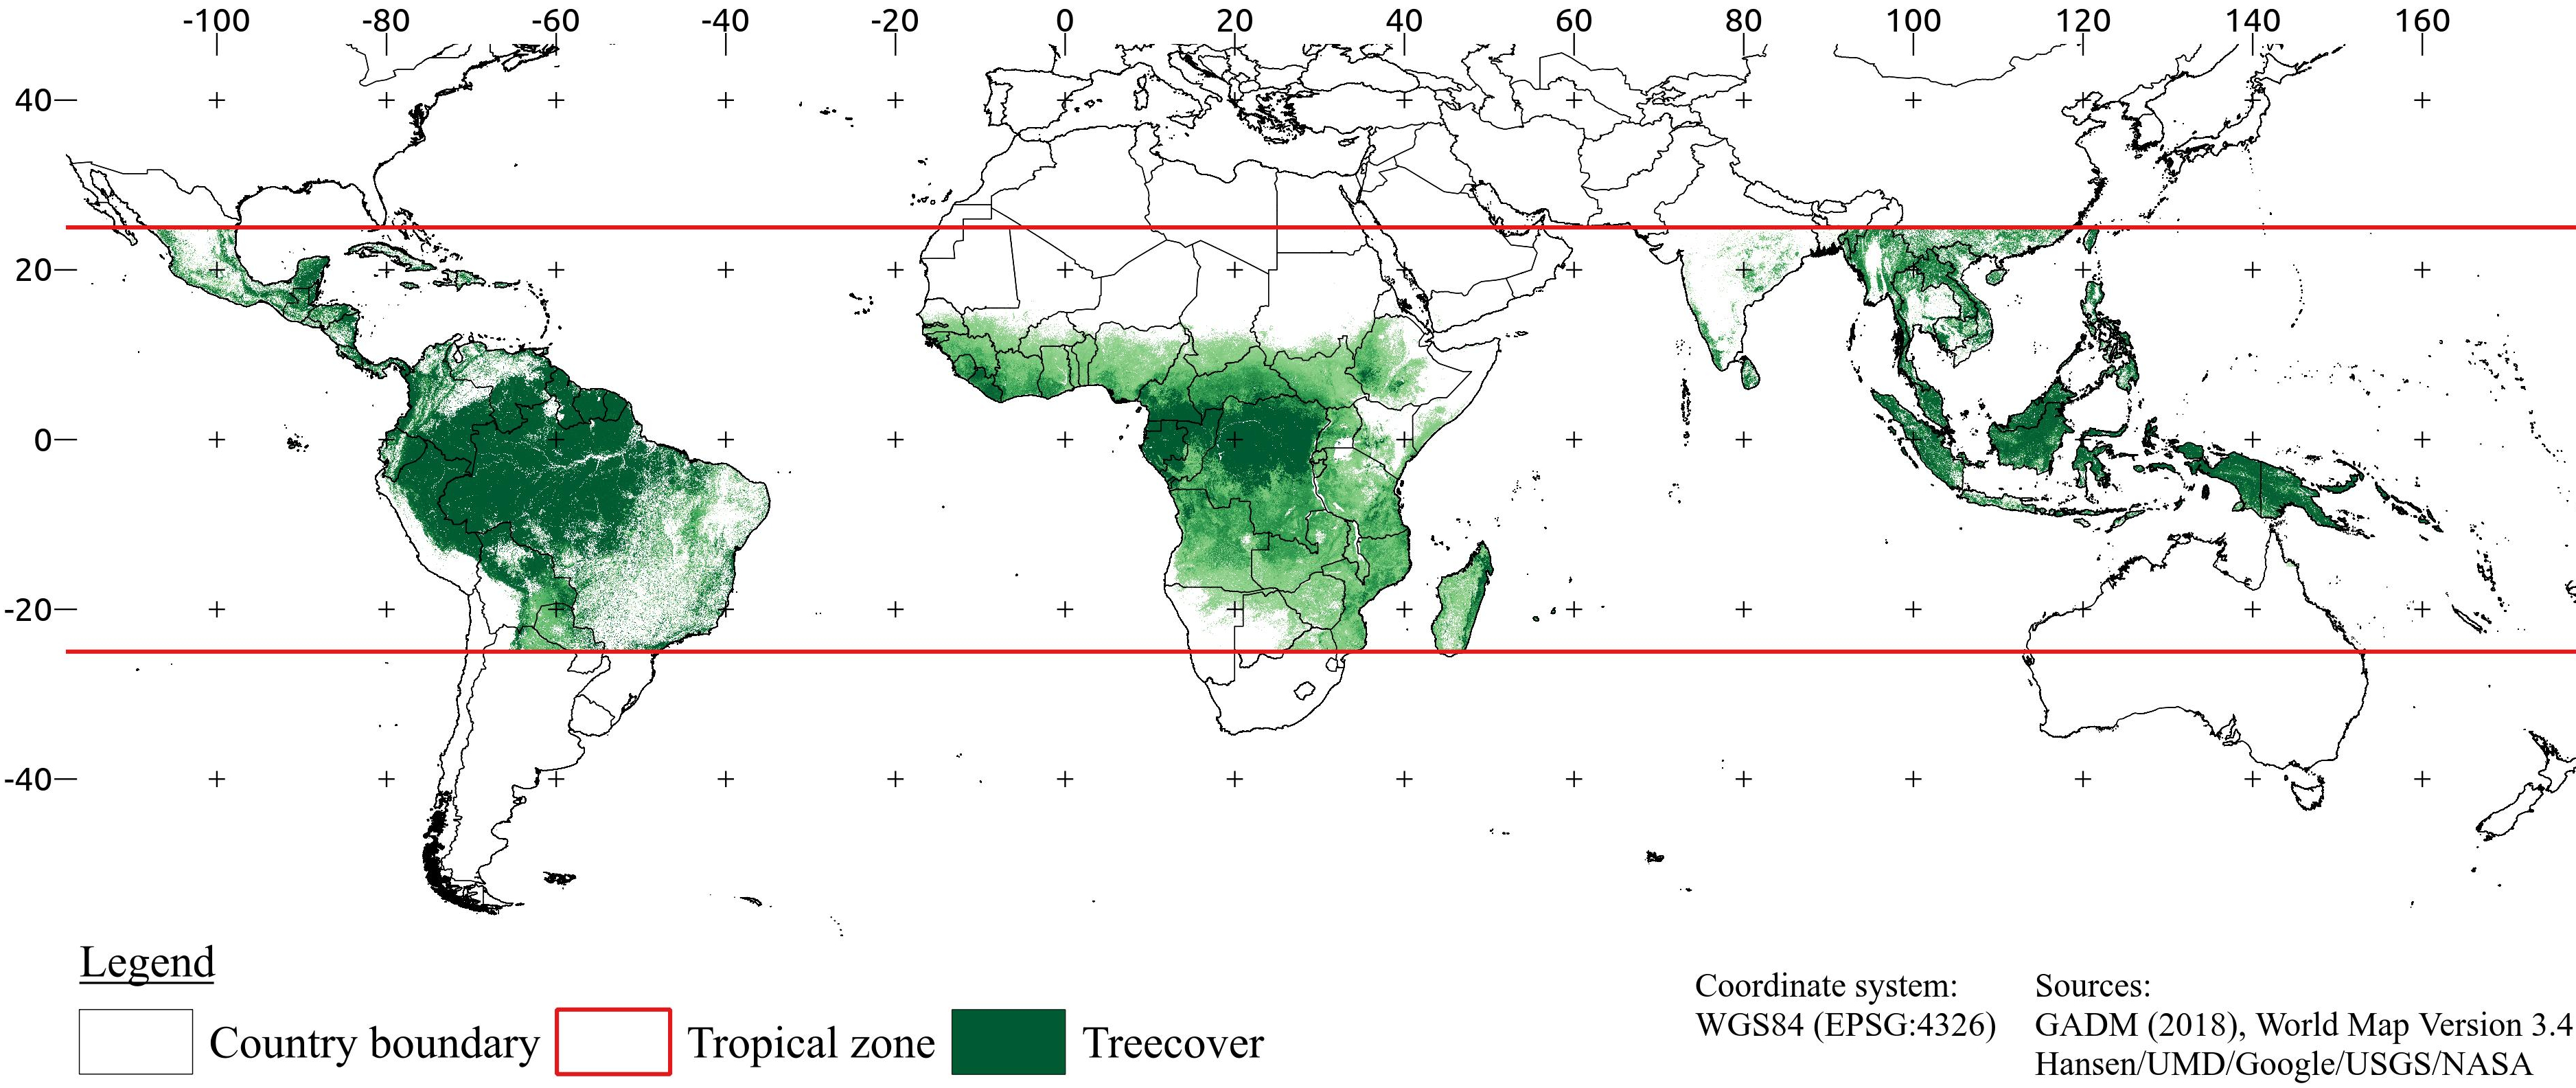
\includegraphics[scale=.97]{img/intro_overview_frameless}
		\caption[Tropical zone and forest]{\textbf{Tropical zone and forest}}
		\label{fig:tropicalzone}
	\end{figure}

% drivers
	Since the 1990s approximately 3.1\% of the global forest area has been lost due to deforestation, while approximately 35\% of the tree cover loss has occurred within the tropical zone \citep{FAO2016}. Between 1990 and 2015 the top ten countries presenting highest annual net loss of forest are concentrated in the tropical belt, which highlights the severe forest alterations within this zone \citep{FAO2010,FAO2016}. Forest loss or deforestation is defined as the removal of trees or forest stands from land surface area, which is then transformed to other LULC (Land use/Land cover) types. Deforestation and LULC change is one of the major causes for the fragmentation of the tropical forest cover \citep{Taubert2018}. Further, tree cover loss is a large emitter of \ac{GHG} emissions \citep{Don2010,Baccini2012}. Additionally, the continuous process of deforestation jeopardizes the carbon fixing capacity of tropical forests \citep{Baccini2017}. Thus it is important to scrutinize the causes of deforestation.

	\citet{Geist2001} introduced the conceptual framework of proximate, underlying, and other causes of tropical deforestation to group the driving forces of forest cover change. The term \ac{PDD} or direct deforestation driver encompass anthropogenic actions that change forest to other \ac{LC} types. Proximate causes of deforestation are subdivided into three different categories: agricultural expansion, wood extraction, and infrastructure expansion. Examples for deforestation driven by agriculture are the expansion of pastures, cropland, and tree crops as exemplified in the figure \ref{fig:deforestationexamples}. The other two categories, wood extraction and infrastructure expansion encompass the following causes: fuelwood extraction, charcoal production, transport infrastructure, and settlement expansion. In contrast, the term underlying causes refers to the complex social, political, economic, technological, and cultural interactions that underpin the \acp{PDD}. The category of other causes for deforestation comprises land characteristics, biophysical drivers, and social trigger events. Features of land characteristics are the soil quality and landscape topography, which could determine the shape and extent of anthropogenic deforestation actions.

	Only a few countries survey \acp{PDD} through a systematic procedure, and spatial analysis are even more rare \citep{Sy2015,Hosonuma2012}. The availability of spatially-explicit data of \acp{PDD} is important because this data can be used to derive other features to describe deforestation comprehensively \citep{Hosonuma2012}. The advances in the field of remote sensing and the availability of country meta-data has fostered the research on \acp{PDD} on a continental or regional scale (e.g. \citet{Sy2015,Austin2019,Zalles2018,Meyfroidt2013,Caldas2013,Graesser2015,Ruf2014,Connette2016,Barima2016,Furumo2017,Vijay2018}). However, the availability of globally-scaled data on direct deforestation drivers is still limited (e.g. \citet{Curtis2018,Hosonuma2012,Geist2002,DeFries2010,Carter2018}). Further, only one study scrutinized the disposition of \acp{PDD} in a spatially-explicit procedure on a global range (e.g. \citet{Curtis2018}).

	All the above-mentioned studies agree on the fact that agricultural expansion dominates the the tree cover loss as \ac{PDD}. Each study estimates a varying size for agricultural causes and other causes, which could be related to differences in the methodology. While, some studies rely on meta-analysis or country meta-data and use an empirical approach to predict \acp{PDD} (e.g. \citet{Hosonuma2012,Geist2002,DeFries2010,Carter2018,Ruf2014}), others apply sample-based methods in combination with statistical models and visual interpretation of remotely sensed data (e.g. \citet{Sy2015,Austin2019,Curtis2018,Meyfroidt2013,Caldas2013}). Additionally, some studies rely only on remote sensing of the environment to predict the proximate causes of deforestation (e.g. \citet{Caldas2013,Zalles2018,Graesser2015,Connette2016,Barima2016}). Further, the studies that estimate the \acp{PDD} in a spatially explicit manner are only available in a low resolution, which can strongly underestimate small-holder deforestation \citep{Curtis2018,Caldas2013}. Additionally, all studies more or less present the proximate causes on deforestation already as aggregates of the three groups that \citet{Geist2001} suggest. Therefore, it is not possible to derive regional or continental differences between the patterns of cropland and pasture expansion.
	\begin{figure}[ht]
		\centering
		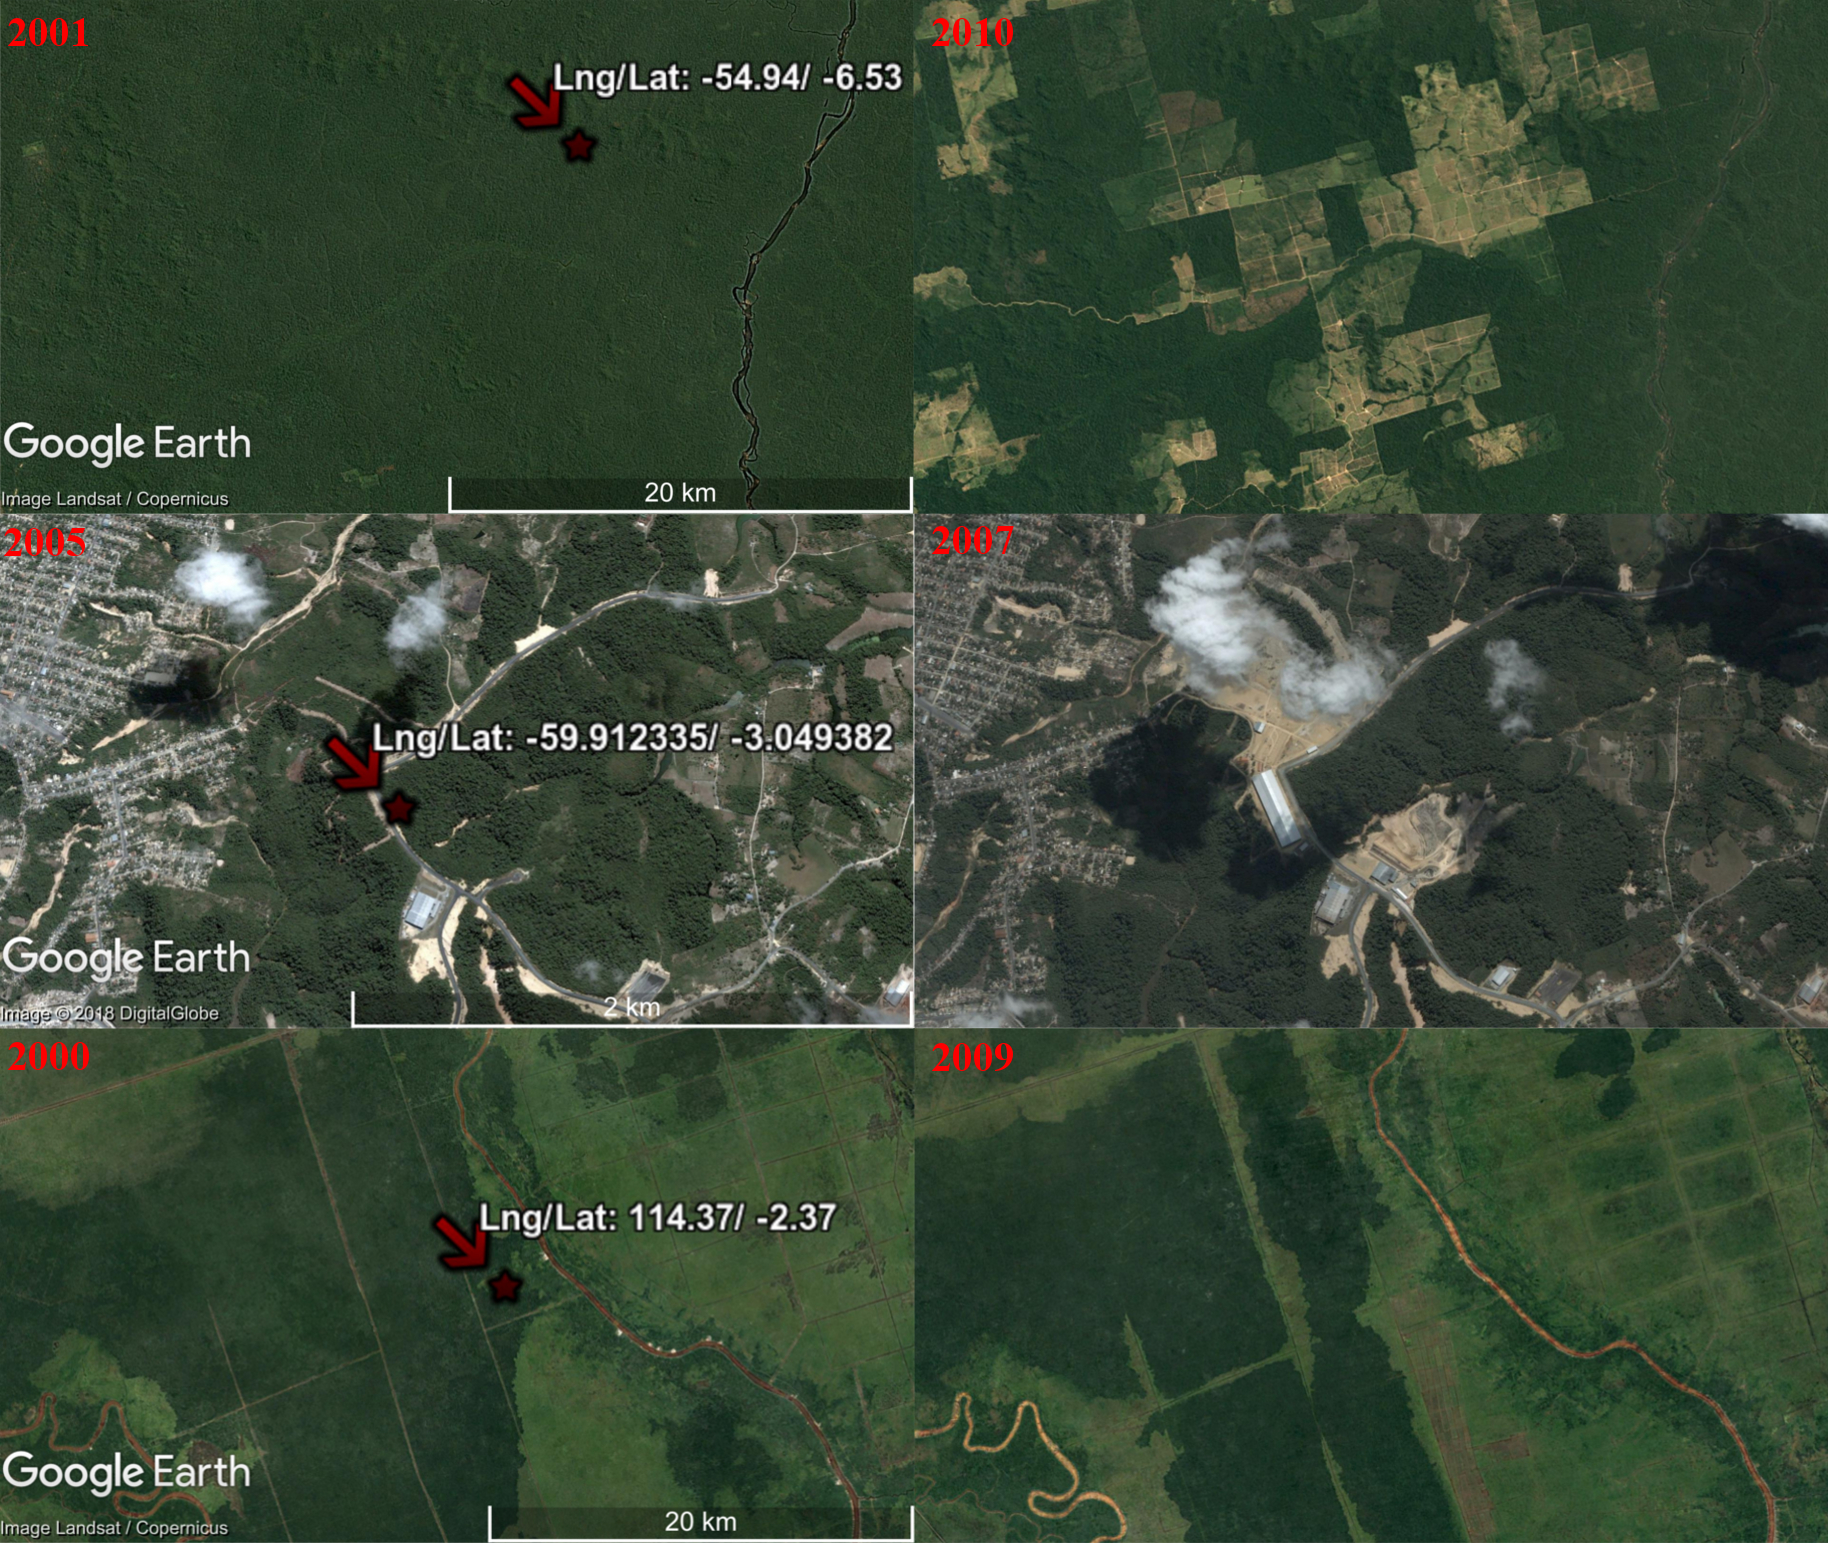
\includegraphics[scale=0.53]{img/deforestation_examples}
		\caption[Examples of proximate deforestation drivers]{\textbf{Examples of proximate deforestation drivers:} The transformation of forests by the expansion of pastures in the Brazilian province of Pará (top), the expansion of settlements in the Brazilian province of Amazonas (center), and the expansion of tree crops (oil palm) in the Indonesian province of Central Kalimantan (bottom).}
		\label{fig:deforestationexamples}
	\end{figure}

% carbon
	The \ac{LC} conversion of tropical forests induced by \acp{PDD} are the second largest source of anthropogenic-induced \ac{GHG} emissions \citep{Don2010}. The main \ac{GHG} released by deforestation to the atmosphere is CO$_2$, which is a major contributor to climate change. Therefore, avoided tropical deforestation could be a significant contribution to climate change mitigation \citep{Don2010}. Further, the United Nations (UN) initiative on Reducing Emissions from Deforestation and Degeneration (REDD+) presents valuable incentives for developing sub-tropical and tropical countries to reduce their emissions from forests \citep{Avitabile2016}. Therefore, carbon emissions accounting plays a key role in the implementation of REDD+ activities.

	The total emissions arising from deforestation can be broken down into many different categories, e.g. \ac{GHG} emissions from biomass removal, emissions resulting from \ac{SOC} dynamics, or the \ac{GHG} emissions arising from the resulting \ac{LU} activity \citep{Avitabile2016}. Carbon emissions from biomass removal arise from aboveground and below-ground biomass of woody vegetation. The quantity of theses emissions is determined by two factors: (1) the rate of deforestation, and (2) the biomass density of the former tree covered area \citep{Houghton2012a}. Carbon loss from \ac{SOC} changes are controlled by two key factors: (1) the decomposition rate of \ac{SOC}, controlled by the surrounding micro-climate, and (2) the variations in the quality and quantity of carbon cycled through the soil system \citep{Don2010}. Deforestation alters both factors and the subsequent \ac{LC} transition controls the soil erosion, which may contribute further to \ac{SOC} loss.

	Tropical soils represent a major carbon storage, which accounts for 30\%-60\% of the carbon stored in forests \citep{Don2010}. Further, tropical vegetation is estimated to store approximately 228.7 Gt C \citep{Baccini2012}. Therefore, it is of outstanding importance to quantify carbon losses by biomass removal and \ac{SOC} change. Studies that estimate the carbon losses by biomass removal on a global or regional scale are common in science, with assessments ranging between 600-1400 Mt C yr$^{-1}$ for 2000-2010 (e.g \citet{Houghton2012,Achard2014,Sy2015,Baccini2012}). Further, several studies scrutinized the impact of different \ac{LC} transition types on \ac{SOC} in terms of carbon losses (e.g. \citet{Don2010,Rahman2018,Villarino2017}). However, no study so far has linked these \ac{SOC} change coefficients to tropical forest \ac{LC} transitions by \acp{PDD} to quantify the total carbon losses. In other words, the \ac{LU} that follows deforestation is typically disregarded in these assessments. Further, it is unknown at which magnitude the \ac{SOC} emissions contribute to the carbon losses by biomass removal.

% esv
	Tropical ecosystems have a crucial impact on the well-being and subsistence of current and future generations through the provision of regulatory, supporting, provisioning, and cultural services \citep{Costanza1997}. Deforestation and \ac{LC} changes lead to major changes in ecosystem services by altering the nature of forest biomes. It is therefore crucial to evaluate these impacts not only in terms of \ac{GHG} emissions but also to account for key ecosystem services such as water regulation, biodiversity, etc. For the quantification of these ecosystem services a economic process is applied to assess the monetary value of each service per ecosystem. These \acp{ESV} can be a strong tool to determine the impact of certain management practices on ecosystem structures. Additionally, it can raise public awareness to the fact that ecosystems are scarce resources, which should not be treated as free, inexhaustible goods \citep{Groot2012}. Further, the valuation of ecosystem services has fostered natural capital accounting and inclusion in national policies \citep{Song2018}. 

	During the past decade scientific research fostered the development of several valuation approaches like direct market valuation, revealed preference, stated preference and benefit transfer \citep{Song2018}. Benefit transfer is the conceptually simplest approach to estimate the \ac{ESV}, but is widely used, especially for estimates over large geographic regions \citep{Costanza1997,Song2018,Costanza2014}. This approach uses a constant unit value per hectare of ecosystem type and multiplies that value by the area of each type to obtain the aggregated total \citep{Costanza2014}. Remotely sensed land cover datasets are widely applied in the estimation \acp{ESV} to derive a global valuation of ecosystems by applying \ac{ESV} unit values \citep{Song2018}.

	The literature provides several studies on ecosystems and its monetary values. However, the most used global unit values for ecosystems by far are the ones prepared by \citet{Costanza2014}. These values have been applied in several studies (e.g. \citet{Costanza2014,Song2018,Sannigrahi2018,Kreuter2001,Wang2006,Zhao2004}). \citet{Siikamaki2015} introduced recently global and regional \ac{ESV} unit values for forest ecosystems. These values are used by the World Bank in its wealth program on developing country-level indicators of sustainability \citep{Siikamaki2015}. Another well known datasets of \acp{ESV} is provided by \citet{Groot2012}. Until now several studies estimated \ac{ESV} dynamics at local or regional scales (e.g. \citet{Kreuter2001,Wang2006,Zhao2004}). Global-scale studies that estimate the monetary value of our planetary ecosystems and the losses by \ac{LC} change are relatively rare (e.g. \citet{Costanza1997,Costanza2014,Sannigrahi2018,Song2018}). The ecosystem estimates of these global studies ranges between 49.4-75.1 trillion dollar per year, while losses due to \ac{LC} change ranges between 1.21-20.2 trillion dollar per year (2007 Int'I\$ yr$^{-1}$). The \ac{ESV} loss due to tropical deforestation ranges between 550.7 billion and 3.5 trillion dollar per year. These estimates are derived from \ac{LC} data at a coarse spatial resolution between 1 km and 300 m except the estimates of \citet{Song2018}, which are derived from the \ac{GFC} dataset at spatial resolution of 30 m. However, the \ac{ESV} accounting of \citet{Song2018} lacks of an importing filtering of the \ac{GFC} data and it does not consider \ac{ESV} dynamics from \ac{LC} change. Therefore, to best of our knowledge no study has accounted for the \ac{ESV} dynamics in regards of \ac{ESV} loss, gain and balance exclusively for tropical forest loss and its \acp{PDD} by using high resolution data.

	\section{Research objectives}
		Based on the research gaps described above we want to focus on the following research questions to analyze tropical deforestation for the 2001-2010 time period:
		\begin{itemize}
			\item What are the proximate drivers of tropical deforestation across different spatial scales?
			\item What are the impacts of tropical deforestation on carbon stocks resulting from biomass removal and \ac{SOC} change?
			\item What are the magnitudes of the ecosystem service value dynamics resulting from tropical deforestation?
		\end{itemize}
%	\newpage
		\chapter{Data and methods}
\label{ch:datamethods}
% TODO introduce what is the content of the chapter
% TODO one idea per paragraph
\section{Data}
\label{sec:data}
% TODO table overview of the data
% TODO put in each dataset section why you use the data as first paragraph/sentence. SO WHAT??? 
	\subsection{Spatial data}
		\subsubsection{Global Forest Change}
			\ac{GFC} 2000-2012 Version 1.0 is the first high-resolution dataset that provides a comprehensive view of the annual global forest cover change between 2000 and 2012 \citep{Hansen2013, Li2017}. The initial \ac{GFC} dataset released by \citeauthor{Hansen2013} is extended by recent releases which encompass the annual forest cover changes between 2000-2013, 2000-2014, 2000-2015 and 2000-2016, respectively. All versions of this dataset have in common, that they are derived from growing season imagery captured by the remote sensing satellite Landsat 7 \ac{ETM+} enhanced by band metrics of other sensors like Quickbird imagery, existing percent tree cover layers from Landsat data, and global \ac{MODIS} percent tree cover \citep{Hansen2013}. On the satellite imagery, a time-series spectral metrics analysis is applied to gather the global forest extent at 2000 as well as the annual forest loss and the accumulated gain for the period 2001 till 2012. Hence, \ac{GFC} comprises three independent data layers tree cover, annually forest loss and forest gain divided into 10x10 degree tiles by the geodetic coordinate system \ac{WGS84} (EPSG:4326) with a spatial resolution of 1 arc-second per pixel (approximately 900 Km$^2$ or 30x30 m). Furthermore, across the provided \ac{GTiff} layers the pixel data is coded in unsigned 8-bit integers. Hansen et al. defined trees as all vegetation taller than 5 meters for their study. For each pixel covered by trees, a canopy density ranging from 0 t0 100 \% is computed. Forest loss is defined as a stand displacement disturbance leading from a forest state to a non-forest state (e.g. canopy density >50 \% to 0). Tree cover gain is defined as the inverse of loss where the canopy density must exceed 50 \% to get recognized.

			\citeauthor{Hansen2013} reports as an accuracy assessment of tree cover loss a producers accuracy of approximately 83 \% for the tropical region. The mapped tree cover gain is probably an underestimation of the true gain with a producers accuracy of 48 \% and a user's accuracy of 81 \%. 

			This dataset is publicly available for download without any constraint. For a convenient bulk download, the dataset homepage provides a "\verb|*.txt|" files comprising the \ac{URL} of the tiles for each sub-dataset. The spatial location of an image can be directly determined from the file name within the \ac{URL}. Each file name has a common pattern shown by the following expression: "\verb|Hansen_VERSION_LAT[NS]_LNG[WE]|". LAT (latitude) and LNG (logitude) refer to the top left corner coordinates of a raster image, whereas these coordinates are only given in natural numbers. The orientation of the image on the hemisphere is determined by the four cardinal directions N (north), S (south), W (west) and E (east). For this project, we require all three sub-datasets, namely: Treecover2000, lossyear, and gain. The data acquisition is automatized with an Python script by using the \ac{stdlib} modules urllib, re, and threading \citep{Rossum2018}. At first, the Python script downloads the provided "\verb|*.txt|" files and creates a list data structure, where each \ac{URL} is element of this list. After, it cycles through the list and extracts the corner coordinates from the file name by means of a \ac{REGEX}. These corner coordinates and cardinal directions are converted to valid latitude and longitude coordinates between $[-90, 90]$ and $[-180, 180]$, respectively. Now, an image is only downloaded if it is within the study extent between $[-20, 30]$ latitude. The acquired image tiles in total 678 are shown in the top panel (green squares) in figure \ref{fig:tiles}. 
			\begin{figure}[ht]
				\centering
				\includegraphics[scale=.93]{img/tiles}
				\caption[Map of downloaded dataset tiles]{\textbf{Map of downloaded dataset tiles:} This map shows the acquired image tiles for this study. From top to bottom in green Global Forest Change (GFC) dataset tiles (Treecover2000, lossyear and gain), the land cover dataset GlobeLand30 (GL30) image tiles in red, and in blue the Aboveground Biomass (AGB) dataset tiles. The orange filled shapes highlight countries within the tropical zone.}
				\label{fig:tiles}
			\end{figure}

		\subsubsection{GlobeLand30}
			\ac{GL30} is the first global land cover dataset with a 30 meter per pixel spatial resolution that provides a comprehensive view on the distribution of 10 different land cover classes (table \ref{tab:gl30classes}) over the entire globe \citep{Chen2017}. Currently this dataset is available for two different time periods 2000 and 2010 \citep{Chen2015}. The pixel values of this dataset are coded in unsigned 8 bit integers and as coordinates system it uses \ac{WGS84} in \ac{UTM} projection. \ac{GL30} can be downloaded as a \ac{GTiff} raster mosaic where each image covers 6x5 degrees \citep{Chen2014}. For detecting the land cover classes \citeauthor{Chen2015} used a so called \ac{POK} oriented approach and satellite imagery from Landsat \ac{ETM+} \citep{Chen2015}. \citeauthor{Chen2015} divided the mapping process in different stages where each land cover type is detected separately and deleted subsequently from the source satellite image. The applied mapping order is: water bodies, wetland, snow and ice, cultivated land and forest, shrubland, grassland and bareland synchronous. To detect the pixels of a selected land cover type the following pixel level classifiers are used: \ac{DT}, \ac{SVM} or \ac{MLC}. After pixel detection the adjacent pixels are grouped as an aggregated land use object. These objects are subsequently validated by expert knowledge and the gained knowledge is used as a feedback loop to improve the automatized classification.

			\citeauthor{Chen2015} estimates an overall mapping accuracy of 80.33 \% and 78.6 \% for 2000 (only validated in Shaanxi, China) and 2010 (global), respectively \citep{Chen2015}. Several research groups besides \citeauthor{Chen2015} validated the mapping accuracy of \ac{GL30} at different regions and scales. \citeauthor{Arsanjani2016} estimates an overall accuracy of 77.9 \% for Iran and an accuracy >80 \% for Germany \citep{Arsanjani2016a,Arsanjani2016}. Yang et al., Cao et al. and Jacobson et al. estimate an accuracy of 82.4 \%, 80.1 \% and 83.1 \% for China, Nepal and East Africa, respectively \citep{Yang2017,Cao2016,Jacobson2015}. Unfortunately, no study focused on validating the mapping accuracy for regions exclusively within the tropical zone.

			\citeauthor{Chen2015} donated the \ac{GL30} land cover mapping to the \ac{UN} but it is not accessible for public download. The download is restricted to users who register on the dataset homepage but the registration process is not working properly. Fortunately the supervisor of this work had already an account otherwise it would be impossible to receive a copy of the dataset. A registered user must fill an order application to get access to the image tiles. The application form must contain the tile identifiers and the selected time period. Tile identifiers have the following common pattern: "\verb|[NS]ZONE_LAT_NAME|" where zone refers to the \ac{UTM} zone between $[1, 60]$, N (north) or S (south) to the cardinal direction, and LAT (latitude) to the latitude coordinate of the top left corner. For a better usability the homepage provides an interface for selecting the required image tiles but the selection of multiple tiles did not work. As well a vector file is provided which contains the dataset tile polygons with assigned identifiers. This file was used to select all required tiles within the tropical zone between approximately $[-23, 23]$ degrees (\ac{WGS84}). Figure \ref{fig:tiles} presents the selected images in red at middle panel. The corresponding image identifiers are converted to an single line string and copied to the application form. After submitting the form the order will be checked and approved within two weeks. After one week we received a two weeks limited access to an password protected \ac{FTP} server where we downloaded 716 raster images. Due to the several restrictions this process of selecting and downloading could not be automatized with one pipeline. Only the selection and string conversion was automatized with a throw away script.
			\begin{table}[ht]
				\centering
				\caption[Classification schema of the GlobeLand30 product]{\textbf{Classification schema of the GlobeLand30 product:} The code column is the assigned pixel value, type the corresponding land cover type and definition explains in broad terms which types of surfaces fall into the land cover type \citep{Chen2017}.}
				\label{tab:gl30classes}
				\begin{tabular}{rlp{10.3cm}}
					\hline
					Code & Type & Definition \\\hline
					10 & Cultivated land & used for agriculture, horticulture and gardens, including paddy fields, irrigated and dry farmland, vegetable and fruit gardens, etc. \\
					20 & Forest & covered by trees, vegetation covers over 30 \%, including deciduous and coniferous forest, and sparse woodland with cover 10-30 \%, etc. \\
					30 & Grassland & covered by natural grass with cover over 10 \%, etc.\\
					40 & Shrubland & covered by shrubs with cover over 30 \%, including deciduous and evergreen shrubs, and desert steppe with cover over 10 \%, etc.\\
					50 & Wetland & covered by wetland plants and water bodies, including inland marsh, lake marsh, river floodplain wetland, forest/shrub wetland, peat bogs, mangrove and salt marsh, etc.\\
					60 & Water bodies & in land area, including river, lake, reservoir, fish pond, etc.\\
					70 & Tundra & covered by lichen, moss, hardy perennial herb and shrubs in the polar regions, including shrub-, herbaceous-, wet- and barren-tundra, etc.\\
					80 & Artificial surfaces & modified by anthropogenic influence, including all kinds of habitation, industrial and mining area, transportation facilities, and interior urban green zones and water bodies, etc.\\
					90 & Bareland & with vegetation cover lower 10 \%, including desert, sandy fields, Gobi, bare rocks, saline and alkaline land, etc.\\
					100 & Snow and ice & covered by permanent snow, glacier and icecap\\\hline
				\end{tabular}
		\end{table}

		\subsubsection{Intact Forest Landscapes}
			A \ac{IFL} is a mosaic of undisturbed forest patches and naturally treeless ecosystems without sings of human activity and large enough to maintain all native biological diversity \citep{Potapov2017}. Due to the fact that \ac{IFL} comprises different intact natural landscape patterns like primary forests, non-forest ecosystems, temporary treeless areas after a natural disturbance, and water bodies the term is not congruent to the term primary forest defined by the \ac{FAO} \citep{FAO2012}. But as mentioned \ac{IFL}s includes large patches of primary forests with a minimum extent of 500 Km$^2$ therefore primary forests can be extracted from the layer. Still there are smaller fragments of primary forest outside of the \ac{IFL}s. In regards of the extent an \ac{IFL} has a minimum size of 500 Km$^2$, a minimum width of 10 Km, and a minimum corridor/appendage width of 2 Km. Further an \ac{IFL} should not contain any of the following: ecosystem alternation, fragmentation by infrastructure and disturbance, and areas altered or managed trough agriculture, logging, and mining. For mapping and detecting \ac{IFL}s \citeauthor{Potapov2017} used Landsat imagery and several auxiliary data sources like \ac{GFC}, and national transportation maps. The dataset can be downloaded as a \ac{SHP} file with the coordinate reference system \ac{WGS84}. Each polygon in the \ac{SHP} represents an \ac{IFL} patch at a certain location on our planet at the time period 2000.

			Data acquisition is pretty straight forward the \ac{IFL} dataset public accessible for download. As mentioned it is an \ac{SHP} so you must only download a single compressed archive. The download is automatized with an Python script by using the \ac{stdlib} modules urllib and threading \citep{Rossum2018}.

		\subsubsection{Aboveground Woody Biomass}
			The \ac{AGB} raster dataset is prepared by \ac{GFW} by an adapted approach of \citeauthor{Baccini2012} \citep{Baccini2012,Baccini2015,Baccini2017}. For the year 2000, this dataset estimates the aboveground biomass density per pixel in Mg C ha$^{-1}$ (mega gram carbon per hectare), and the confidence per pixel at a spatial resolution of approximately 1 arc-second (approximately 900 Km$^2$ or 30x30 meter). The dataset covering the global tropical zone as an mosaic of \ac{GTiff} raster images where each tile of the mosaic has the \ac{CRS} \ac{WGS84} and is coded in float. For deriving biomass density \ac{GFW} used canopy metrics from \ac{GLAS} \ac{LIDAR} footprints and several regional and forest specific allometric equations. The resulting \ac{GLAS} \ac{AGB} estimates are used as labels to train regional specific \ac{RF} models based on Landsat 7 \ac{ETM+} top-of-atmosphere reflectance, tree canopy density of \ac{GFC}, elevation data, and climate data as predictor variables. After these models are subsequently applied to the entire study extent to predict the biomass content for each pixel. Additional a uncertainty layer is prepared accounting for the errors from allometric equations, the \ac{LIDAR} based model, and the random forest model.

			The \ac{AGB} raster mosaic is public available on the homepage of \ac{GFW}. As mentioned, the dataset covers only the tropical zone, therefore we acquires the entire mosaic. The \ac{GFW} homepage provides an \ac{GeoJSON} \ac{API} to receive the actual \ac{URL} of each raster image. If a request is send to this \ac{API} the server response with a \ac{GeoJSON} feature collection. The collection contains as attributes the \ac{URL}s of the biomass images, the \ac{URL} of the uncertainty layers, and the rectangular bounds of each image. The data acquisition is automatized by means of Python and the \ac{stdlib} modules urllib, threading, and the open source library geopandas \citep{Rossum2018,McKinney2010}. At first the \ac{GeoJSON} is downloaded via an \ac{API} call and eventually stored on disk. Next we iterate the features of the \ac{GeoJSON} collection and extract the \ac{URL}s (biomass and uncertainty) of each tile. These \ac{URL}s are downloaded and subsequently stored on disk. During the downloads of the uncertainty layers the \ac{GFW} server answered repeatedly with a 404 (Not found). Therefore the uncertainty layers are not available. In total we downloaded 105 different image tiles, their extent and spatial location is shown in blue at the bottom panel of figure \ref{fig:tiles}.

		\subsubsection{Global Soil Organic Carbon}
			% TODO references for wosis, hwsd, and other data products
			The \ac{GSOCmap} is a joint project between \ac{GSP} and \ac{ITPS} to produce a global \ac{SOC} content map by a country driven approach. In the year 2018, the first iteration of this map in version 1.0 was released, and shortly followed by 1.1 (new country submission by Rwanda) and 1.2 (new country submissions by Chile and Colombia). As the short release cycle suggests the mapping project is intended as a long-lived dataset which will improve over time and by new country submissions. Till now 67 (approximately 63 \% of the global land mass) different countries submitted their country based \ac{SOC} estimates. To foster the national \ac{SOC} mappings the \ac{ISRIC} provides several covariate datasets like national \ac{DEM} maps, annual spectral remote sensing data or national soil type grids. Additionally the contributors can join a mapping training and use the \ac{GSOCmap} cookbook as guidance for their mapping efforts. As an exchange, each country shares its national \ac{GSOCmap} by compliance of several criteria e.g. reporting of the Meta-data of the \ac{SOC} sampling (sample timeline, sample depth, bulk density etc.), uncertainty assessment, and the applied methods for estimating and interpolation of the \ac{SOC} content. For interpolating the guide organizations suggest the following approaches: simple geo-matching, class-matching, \ac{MLR}, \ac{RF} or \ac{SVM}. The national maps are aggregated to the final \ac{GSOCmap} with a target resolution of 30 arc-seconds (approximately 1 Km$^2$) in the \ac{CRS} \ac{WGS84}. The dataset is one single raster image as \ac{GTiff} coded in float covering the entire globe where each pixel value is the \ac{SOC} content in Mg C ha$^{-1}$ at a soil depth of 0-30 cm \citep{FAO2018}.

			The product is validated by comparing the pixel level estimates with soil sampling data from various soil databases (WoSIS, HWSD, etc.). In total 312122 samples where divided into three sub-levels (<150 Mg C ha$^{-1}$, >150 Mg C ha$^{-1}$, and all samples) and subsequently computed the \ac{ME}. The \ac{ME} of the entire sample space and <150 Mg C ha$^{-1}$ suggests that the mean \ac{SOCC} estimate is an overestimate of 1.6 and 4.5 Mg C ha$^{-1}$ respectively. All samples with a \ac{SOCC} content >150 Mg C ha$^{-1}$ show an underestimate by approximately 165 Mg C ha$^{-1}$ in the mean. Additionally, an uncertainty assessment was prepared to estimate a \ac{SD} between $\pm$ 0-16 t ha$^{-1}$ for the tropical zone. Unfortunately, is this assessment pretty rough and till now not available as a product. The \ac{GSOCmap} in comparison with other global \ac{SOC} products has the lowest \ac{RMSE}. In summary, the prepared validations show evidence that the \ac{GSOCmap} is a conservative data product with a tendency to underestimate the \ac{SOCC}.

			The dataset is publicly available at the homepage of the \ac{FAO}. As mentioned it consists of one raster image, therefore we download it by means of a Python script without any additional steps.

		\subsubsection{Auxiliary}
			As auxiliary data for country boundaries we downloaded with Python the \ac{GADM} layers as \ac{SHP} files \citep{Hijmans2018,Rossum2018}.

	\subsection{Empirical data}
		\subsubsection{Soil Organic Carbon}
			\citeauthor{Don2010} performed the first study of tropical \ac{SOC} change for soil depth between 0 and 30 cm. For the study a global meta-analysis is applied by using 358 (153 published an peer-reviewed) different studies to estimate \ac{SOC} change for 12 major \ac{LUC} types. The base date is derived from 39 different tropical countries covering all continents. Unfortunately Africa and East-Asia are under-sampled whereas South-America have the best data coverage. The meta-analysis is restricted to mineral soils therefore all wet soil types are excluded from the analysis \citeauthor{Don2010}. The 12 \ac{LC} transitions encompass the following \ac{LC} types: primary forest, secondary forest, grassland, cropland, and perennial crops. Primary forest are defined as natural vegetation without human impacts which includes natural grassland and shrubland. Secondary forest are managed forests and regrown forests after partial destruction of the old stand. Grassland comprises pastures for livestock but excludes natural grasslands. Cropland comprises annual crops like maize or beans and perennial crops could be coffee or sugar cane. For our study we used only the \ac{SOC} change estimates for these \ac{LUC} types which corresponds to the \ac{GL30} and \ac{IFL} classification schema. The actual values are shown in table \ref{tab:soc}.
			\begin{table}[ht]
				\centering
				\caption[Relative soil organic carbon change for certain land-use change types]{\textbf{Relative soil organic carbon change for certain land-use change types:} The Land-use change columns from and to define the LUC type with the corresponding relative Soil Organic Carbon (SOC) change and the Standard Error of the Mean (SEM) \citep{Don2010}.}
				\label{tab:soc}
				\begin{tabular}{ccrr}
					\hline
					\multicolumn{2}{c}{LUC type} & \multicolumn{2}{c}{Relative SOC change} \\
					From & To & [\%] & SEM \\\hline
					Primary forest & Grassland & -12.1 & $\pm$2.3 \\
					Primary forest & Cropland & -25.2 & $\pm$3.3 \\
					Primary forest & Secondary forest & -8.6 & $\pm$2.0 \\
					Secondary forest & Grassland & -6.4 & $\pm$2.5 \\
					Secondary forest & Cropland & -21.3 & $\pm$4.1 \\\hline
				\end{tabular}
			\end{table}

		\subsubsection{Ecosystem Service Values}
		% TODO write the section, improve caption
			Some text to ensure document flow.
			\begin{table}[ht]
				\centering
				\caption[Selection of Ecosystem Service Values (ESV) used in this study]{\textbf{Selection of Ecosystem Service Values (ESV) per biome used in this study:} ESV per biome connected with the corresponding GlobeLand30 land-cover class, and its monetary value in Int.\$ ha$^-1$. Dg refers to data from \citeauthor{Groot2012}, Co from \citeauthor{Costanza2014}, and Wb from \citeauthor{Siikamaki2015}.\citep{Groot2012,Costanza2014,Siikamaki2015}}
				\label{tab:esv}
				\begin{tabular}{lclrrr}
					\hline
					Biome & Code & Type & Dg & Co & Wb \\\hline
					Cropland & 10 & Cropland & - & 5,567 & -\\
					Forest tropical & 20 & Forest & 5,264 & 5,382 & 1,312\\
					Forest tropical & 25 & Regrowth & 5,264 & 5,382 & 1,312\\
					Grass/Rangelands & 30 & Grassland & 2,871 & 4166 & -\\
					Wetlands & 50 & Wetland & 25,682 & 140,174 & -\\
					Lakes/Rivers & 60 & Water bodies & 4,267 & 12,512 & -\\
					Urban & 80 & Artificial & - & 6,661 & -\\\hline
				\end{tabular}
			\end{table}

\section{Methods}
\label{sec:methods}
%TODO need more speacking section headings
% TODO put in each dataset section why you use the data as first paragraph/sentence. SO WHAT???
	\subsection{Preprocessing}
		%TODO improve flowchart final masking, improve caption
		Before we apply further analysis, we have to generalize the used datasets. As introduced in the data section do we use datasets which differ largely in their metadata properties, for example, single-tiled or multi-tiled images, used \ac{CRS}, spatial resolution, and file type. Therefore, our goal should be to develop a process which creates an image stack of equal meta-data for each location in our study extent. In further descriptions, we will refer to this stack as \ac{AISM}. As target \ac{CRS} for our \ac{AISM} we chose \ac{WGS84} and as target extent for the mosaic, we use the bounding box of the \ac{GL30}-2010 tiles. The following paragraph explains how we developed the alignment algorithm by means of Python and the additional open source libraries rasterio, geopandas, and shapely \citep{Rossum2018,McKinney2010}.

		The first exercise of the preprocessing algorithm is to detect all tiles covering the extent of our template tiles. At first, we create for each multi-tiled dataset a polygon mask as \ac{SHP}. This mask contains the spatial extent of each tile within a dataset and as attribute the corresponding file identifier. If the dataset tiles are not in \ac{WGS84} the extracted bounds are subsequently reprojected to this \ac{CRS}. During the masking process, we recognized that the raster mosaic bounds of both \ac{GL30} datasets (2000 and 2010) generate re-projection errors. These errors showed up as polygons spanning the entire globe but one tile can only fill its \ac{UTM} zone extent. A further analysis revealed that all tiles located in \ac{UTM} zone 1 and 60 overflowing the maximum and minimum longitude coordinates of this zones. As solution we excluded all tiles within \ac{UTM} zone 1 and 60 from further processing, namely: n01\_00, s01\_00, s01\_10, s01\_15, s01\_20, s60\_00, s60\_05, s60\_10, s60\_15, and n53\_00. The described steps can be found as well in figure \ref{fig:preprocessing_flowchart}. Now, as the figure suggests we determine the intersection between these mask layers and group the intersecting tiles by our template tile. Next, we create for the template tile a re-projection profile (warp profile) and apply it subsequently to all intersecting tiles based on the following rules: if from one dataset more than one tile intersects merge them followed by re-projection or if only one tile intersects just re-project it. As introduced the \ac{GSOCmap} consist only of one single tile with a spatial resolution of approximately 1 Km$^2$, so it must only re-project and re-sampled by nearest-neighbor approach. We select from the \ac{IFL} layer all polygons within our template warp profile and convert them to a raster layer where intact forest patches are coded by a one in 8-bit unsigned integer. Last step of the alignment process is the rounding of the \ac{AISM} bounds to full integer degrees and a subsequent clipping of each tile to this rounded bounds. The entire work flow it pictured in figure \ref{fig:preprocessing_flowchart} and results in a \ac{AISM} shown in figure \ref{fig:aism}. Finally, we create a polygon mask of our \ac{AISM} and store for each polygon the corresponding dataset tiles. This mask is used as a file index for the next algorithms.
		\begin{figure}[ht]
			\centering
			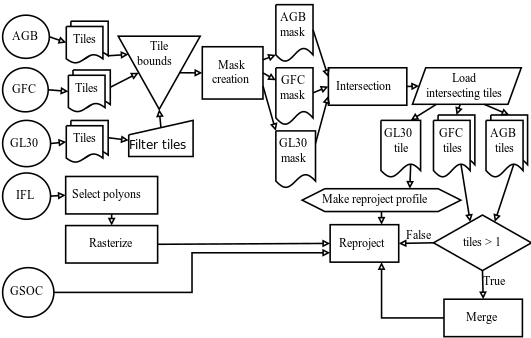
\includegraphics[scale=.8]{img/align}
			\caption[Flowchart of tile alignment process]{\textbf{Flowchart of tile alignment process:} For the multi-tiled datasets (multi-document symbols) a mask is created by extracting the tile bounds. Next, the intersection between theses masks is determined and the corresponding tiles are loaded from disk. \ac{GL30} tiles are used as template by creating re-project profile and subsequently applying it to intersecting tiles. From the \ac{IFL} layer only polygons within the re-project are selected and subsequently converted to a raster layer.}
			\label{fig:preprocessing_flowchart}
		\end{figure}
		\begin{figure}[ht]
			\centering
			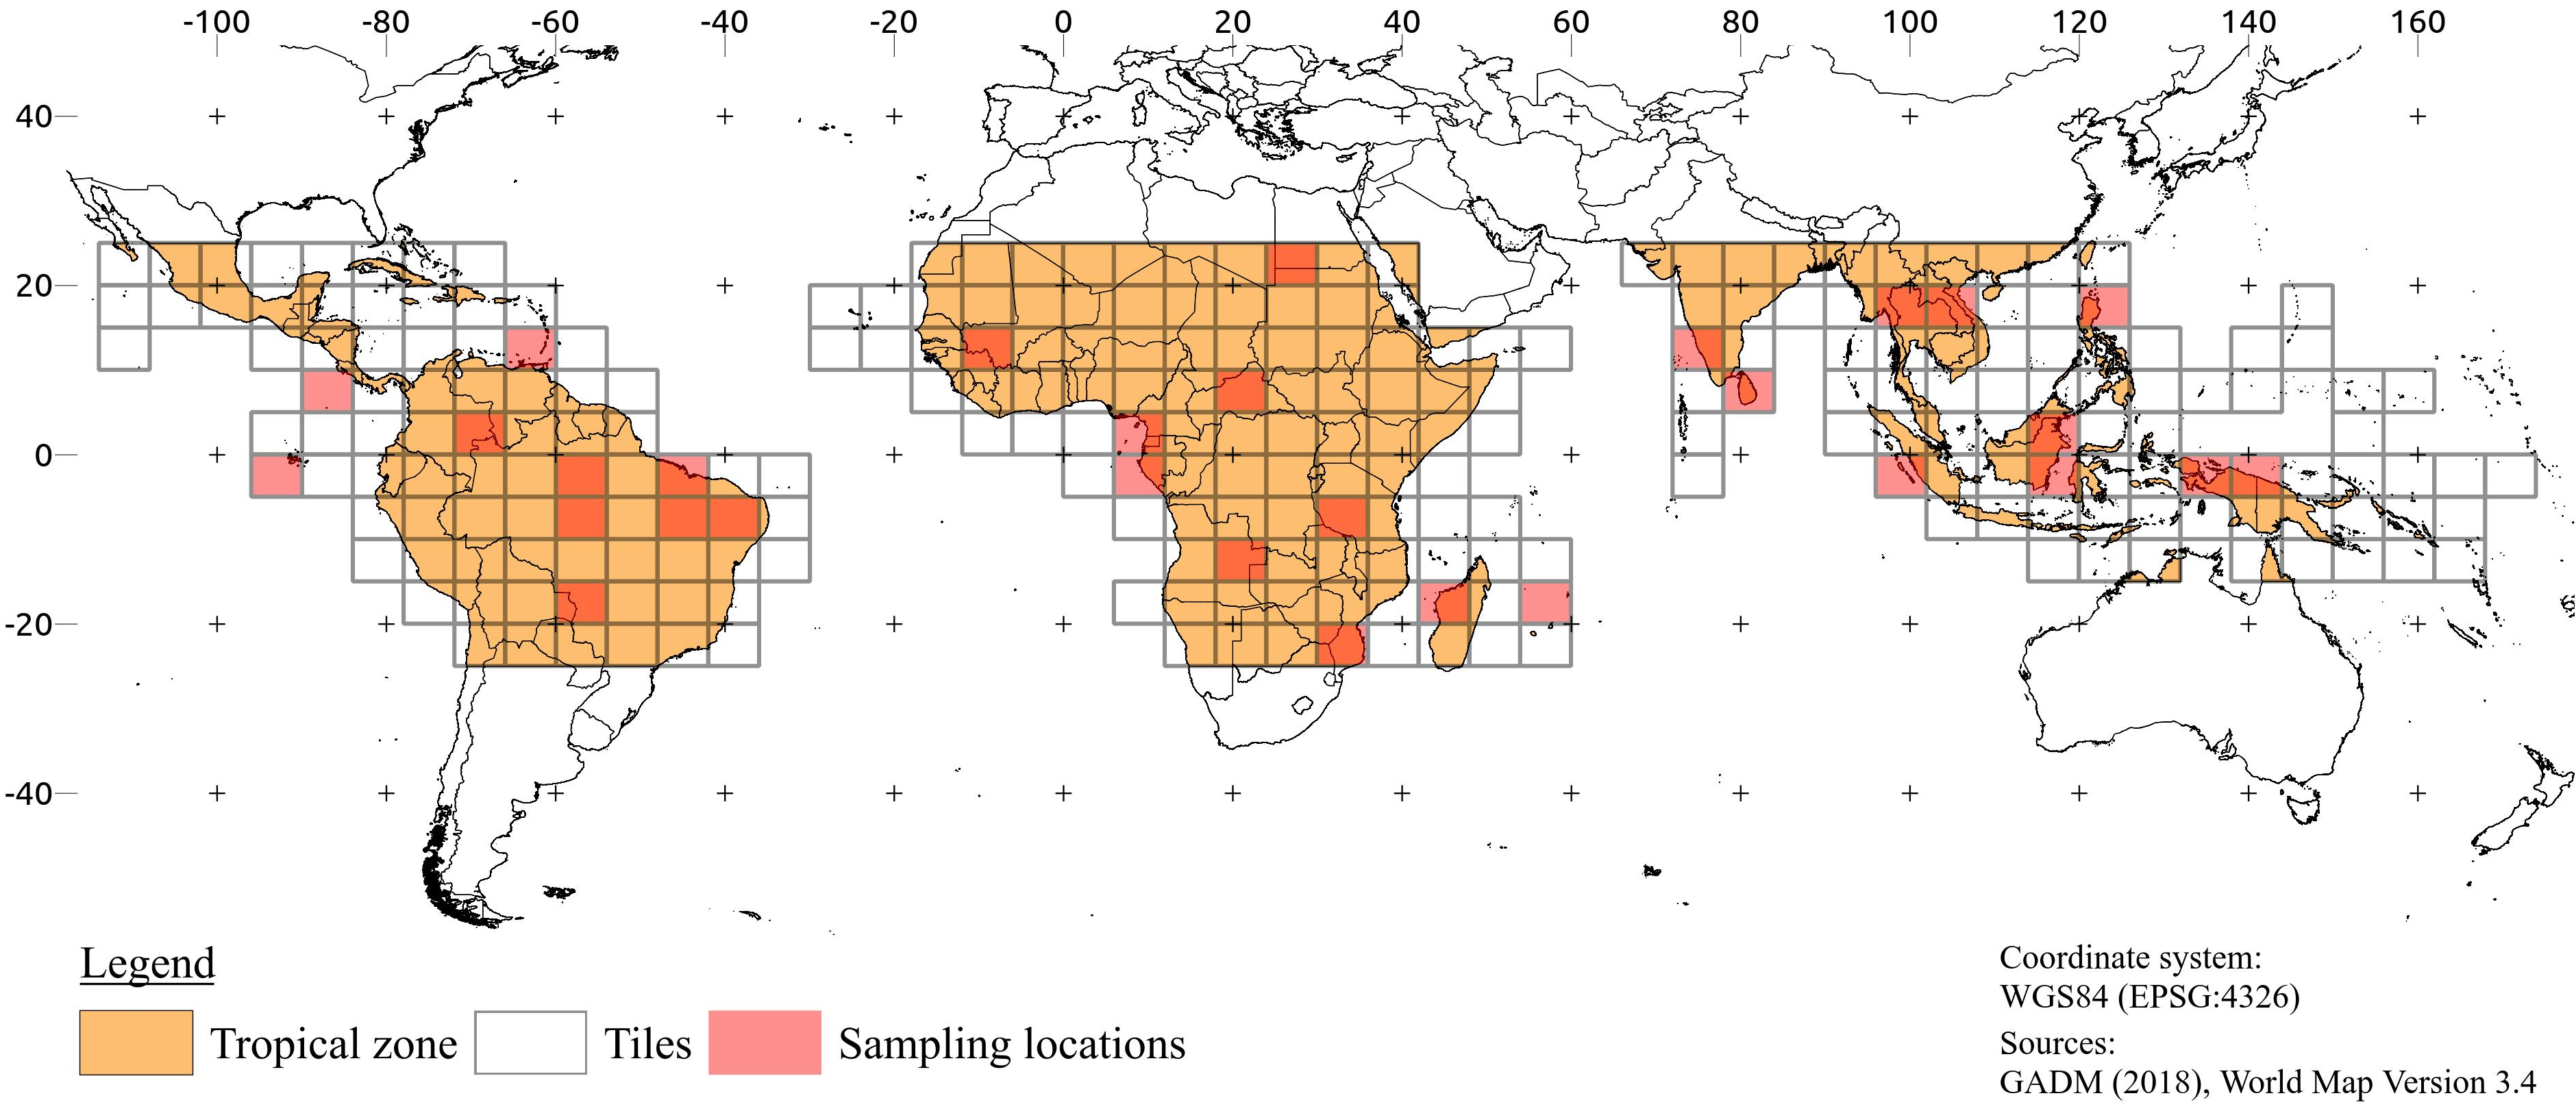
\includegraphics[scale=.91]{img/method_overview_frameless}
			\caption[Map of aligned data tiles and sampling locations]{\textbf{Map of aligned data tiles and sampling locations:} The map shows the location of the aligned multi-image stack tiles as black-framed square sized polygons, the sampling locations for accuracy assessment in red, and countries within the tropical zone in orange.}
			\label{fig:aism}
		\end{figure}

	\subsection{Deforestation}
		\subsubsection{Forest definition}
			%TODO equations
			Goal:
			We aggregate two layers. Both have slightly different definitions for tree cover. To successful aggregate the layers we must harmonize the tree cover situation between the gfc tree cover and the gl30 2000 treecover. Because we want to map changes both have to agree on tree cover.

			Similarity:
			To determine the similarity between gl30 and gfd tree cover we used jaccard index. Jaccard Index (coefficient of community) is a simple measure of similarity between two binary paired populations or the measure of the degree of spatial overlap between two images. First applied by Jaccard in 1912 to compare distributions of alpine flora. Properties of Jaccard if a is zero jaccard is zero if b and c are zero jaccard is one. value range between 0 and 1 and relationship between s(ij) and a near linear. Process we computed subsequently for each image tile the jaccard index. First step is to filter gl30 map for tree cover. Next we compute the jaccard index  The process is implement as binary operations (a = x or y, abc = x or y, b = x xor a, c = y xor a, d = not x and not y) by means of numpy and python.

			Hypothesis testing:

			Treecover agreement: Jaccard index first applied for a study on plant distribution similarities at different locations in alps and developend by jaccard \citep{Jaccard1912,Shi1993,Sampat2009} jaccard index, wilcoxon signed-rank test, gl30 2000, gfc treecover 2000, different canopy densities JI$_0$$[0,100]$, JI$_{1}$$(10,100]$, JI$_{2}$$(20,100]$, JI$_{3}$$(30,100]$ 

		\subsubsection{Proximate deforestation driver}
			%TODO flowchart needs reclassification
			Based on our forest definition developed in the previous section we want to classify all the tropical deforestation within a canopy density of $(10,100]$ percent between 2001 till 2010. Additionally we must consider the mean miss-classification rate of 52 \% by previous findings of \citeauthor{Seydewitz2017} \citep{Seydewitz2017}. Therefore we have to develop a feasible method to resolve this issue.

			For classifying the proximate drivers of deforestation we select the following raster images from our \ac{AISM}: \ac{GFC} treecover2000, \ac{GFC} lossyear, \ac{GFC} gain, and the \ac{GL30} \ac{LC} classification from 2010. Now, we apply to each raster image stack the following described operations. From the treecover2000 layer we select all pixels where the canopy density is within $(10,100]$ percent and set them to one (true). The same is procedure is applied on the lossyear layer by setting all forest loss pixels within the time period 2001 till 2010 to one (true). After both layers are combined with a logical AND to select our target deforestation pixels. Finally, we build the Hadamard product (element-wise multiplication) of the target deforestation layer and the \ac{GL30} \ac{LC} layer to classify the deforestation pixels. For classifying forest regrowth we filtered the \ac{GFC} gain layer by forest gains within our target temporal resolution and losses within our target canopy density. After, the filtered gains are aggregated with our classified deforestation by using the Hadamard product of both layers. Figure \ref{fig:driver_flowchart} shows the classification process as a flowchart. The classification process is implemented as a Python function which requires as parameter the previously named raster layers. Additionally the target canopy density and time period is freely selectable. The described filtering and aggregation steps are implements as binary operations for fast processing by means of numpy.

			Clustering of all patches still classified as forest (value 20), apply square sized buffer around cluster center, count occurrences of other classes within the buffer, apply to cluster most frequent class, exclude from counting 20, 0, and 255, buffer size 500x500 m 25 ha.
			\begin{figure}[ht]
				\centering
				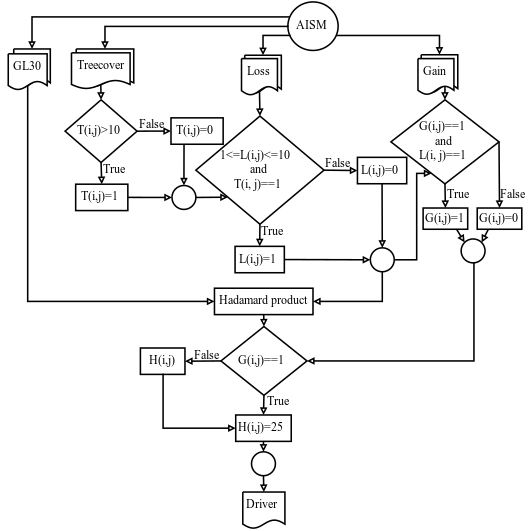
\includegraphics[scale=0.5]{img/driver_flowchart}
				\caption[]{\textbf{Title:}}
				\label{fig:driver_flowchart}
			\end{figure}

		\subsubsection{Accuracy assessment}
			For examining the accuracy of our proximate deforestation driver prediction we used a confusion matrix (also known as two-way frequency tables, error matrix or contingency tables). These matrices are commonly used for an accuracy assessment of land cover classifications and enables the computation of marginal and conditional distributions \citep{Congalton1991,Foody2002}. Table \ref{tab:confusion} shows a general model of a confusion matrix. Foundation for an accuracy assessment by means of a confusion matrix is a collection of ground-truth samples which can be compared with the class predictions for these samples produced by a classification algorithm. For the preparation of our accuracy assessment, we have to extract a collection of pixel samples with a deforestation occurrence from our proximate  driver maps (further also called predictions). Next, we compose a set of ground-truth for these predictions (further also called references).
			\begin{table}[ht]
				\centering
				\caption[A general model of a confusion matrix]{\textbf{A general model of a confusion matrix:} $X_1$, ... , $X_n$ denote classification categories of two independent raters. $x_{n,n}$ are the actual samples sorted into the categories where the values in the diagonal show the agreement between both raters. The remaining cell values account for the disagreement between the two raters. $\sum$ column and row show the marginal distribution and N is the total number of samples.}
				\label{tab:confusion}
				\begin{tabular}{lccccc}
					\hline
					& & \multicolumn{3}{c}{Reference} & \\
					& Cls & $X_1$ & $\cdots$ & $X_n$ & $\sum$ \\\hline
					\multirow{4}{*}{\STAB{\rotatebox[origin=c]{90}{Predict}}}
					& $X_1$ & $x_{1,1}$ & $\cdots$ & $x_{1,n}$ & $x_{1.}=
					\displaystyle\sum_{i=1}^{n} x_{1,i}$ \\ 
					& $\vdots$ & $\vdots$ & $\ddots$ & $\vdots$ & $\vdots$ \\ 
					& $X_n$ & $x_{n,1}$ & $\cdots$ & $x_{n,n}$ & $x_{n.}=\displaystyle\sum_{i=1}^{n}x_{n,i}$ \\\hline 
					& $\sum$ & $x_{.1}=\displaystyle\sum_{i=1}^{n}x_{i,1}$ & $\cdots$ & $x_{.n}=\displaystyle\sum_{i=1}^{n}x_{i,n}$ & $\sum\sum=N$ \\\hline
				\end{tabular}
			\end{table}

			To create our collection of ground-truth data we draw randomly 10 image tiles from all three continental regions (Latin America, Africa, Asia/Oceania). From each tile, we sampled by random 200 pixels which total to 6000 samples over the entire study region. The sampling is realized with our own raster sampling algorithm build in Python by means of the open source libraries numpy and rasterio. As mentioned in the previous section do we superimpose two datasets and only a certain amount of pixels per tile is classified as proximate driver. Therefore, the sampling algorithm should only draw samples from occupied/classified pixels without replacement. The algorithm expects as parameters a raster image, the total number of samples to draw, a list of pixel values which should be interpreted as occupied cells, the affine transformation matrix of the raster image, and a seed for the random number generator. If occupied cells are set the algorithm will create a binary mask where each occupied cell is set to one relative to the input raster image. Otherwise it sets all pixel values greater or less than zero to one. After, the row and column coordinates of each one are extracted from the mask and converted to a flat list of coordinate tuples. Next, it draws the predefined number of samples from the list by a random order and uses the image coordinates to get the pixel value from the raster image. If a affine transformation matrix is provided the image coordinates are converted to real world coordinates. The seed argument ensures that on every algorithm rerun the samples are drawn. For our sampling we set the parameters to the following values: samples 200, occupied pixels \ac{GL30} class values and 25 for regrowth, affine matrix of the corresponding raster image, and the seed is 42. The per tile samples are stored as an \ac{CSV} file.

			For the collection of ground-truth data we used visual interpretation of Google Earth satellite and aerial imagery. We developed a small JavaScript web application to access the imagery via the Google Maps \ac{API}. The application expects as input a \ac{CSV} file with the sampling coordinates. After upload of a sample file the user can cycle trough the entries and the map jumps automatically to the coordinates of the sample. Now a reference label can be assigned to the coordinates by visual interpretation of the imagery. We subsequently assigned to all 6000 samples a reference label and downloaded the results as \ac{CSV}.

			Finally, we developed a Python class to compute the confusion matrix. The constructor of the class requires a list of reference and prediction labels. With the provided arguments it creates the confusion matrix. Further, it computes the following marginal and conditional distributions: overall accuracy $OvAc$ by dividing the sum of classification agreements trough the sample total $N$ (equation \ref{eq:OvAc}), the producer accuracy $PAc_{.n}$ by dividing the category agreement trough the column category total (equation \ref{eq:PAc}), the error of commission $Com_{.n}$ (Type II error) by dividing the category disagreement trough the column category total (equation \ref{eq:Com}), the user accuracy $UAc_{n.}$ by dividing the category agreement trough the row category total (equation \ref{eq:UAc}), the error of omission $Om_{.n}$ (Type I error) by dividing the category disagreement trough the row category total (equation \ref{eq:Om}), and the Cohens Kappa by substituting equation \ref{eq:cohen} and \ref{eq:OvAc} into equation \ref{eq:Kappa}.
			\begin{equation}
			\label{eq:OvAc}
				p_0=OvAc = \frac{\displaystyle\sum_{i=1}^{n}x_{i,i}}{N}
			\end{equation}
			\begin{equation}
			\label{eq:PAc}
				PAc_{.n} = \frac{x_{i,i}}{x_{.n}}
			\end{equation}
			\begin{equation}
			\label{eq:Com}
				Com_{.n} = \frac{FN_i}{x_{.n}}
			\end{equation}
			\begin{equation}
			\label{eq:UAc}
				UAc_{n.} = \frac{x_{i,i}}{x_{n.}}
			\end{equation}
			\begin{equation}
			\label{eq:Om}
				Om_{n.} = \frac{FP_i}{x_{n.}}
			\end{equation}
			\begin{equation}
			\label{eq:cohen}
				p_c = \frac{1}{N^2}\displaystyle\sum_{i=1}^{n} x_{.i} \cdot x_{i.}
			\end{equation}
			\begin{equation}
			\label{eq:Kappa}
				Kappa = \frac{p_0-p_c}{1-p_c}
			\end{equation}

	\subsection{Emissions}
		\subsubsection{Above ground biomass}
			\lipsum[1-2]
		\subsubsection{Soil organic carbon change}
			\lipsum[1-2]

	\subsection{Ecosystem service values}
		\subsubsection{Ecosystem service value loss}
			\lipsum[1-2]
		\subsubsection{Ecosystem service value gain}
			\lipsum[1]

	\subsection{Binning analysis}
		% TODO REVIEW, CHANGE TO GOOD ENGLISH
		The previous sections were focused on the generation of large scale spatial data. Now, a feasible method must be developed for analyzing, aggregating, interpreting, and visualizing our results. For the development of a proper approach we have to generalize the problem domain. At first we are confronted with large N (many samples) which results in a high dimensionality and complexity of relationships among this variables \citep{Carr1990}. From a visual/analytical perspective georeferenced raster maps can be interpreted as a multivariate scatter plot of large datasets where longitude and latitude represent the x and y coordinate of an data point and the pixel values (in this case nominal scaled) representing the third dimension as an group coloring. Therefore we have a large multidimensional dataset combined with a scatter plot visualization which leads commonly to over plotting issues and hidden point densities \citep{Carr1987}. Due to the spatial nature of your data we are also confronted with not equal distributed data some regions show high data densities and other regions have sparse to no data. Also a severe problem domain is the frame size of our representation. Goal is to present data on a continental level which intensifies visual problems. Each pixel has a resolution of approximately 30x30m, the continental representation of americas spanning approximately 1200000x120000km2. Therefore small scale isolated changes are hidden and only large scale changes are visual detectable. Which results in hidden details and not perceivable patterns of change.

		% TODO REFERENCE FOR MAJOR RESAMPLING APPROACH
		% TODO DESCRIBE ADVANTAGES DISADVANTAGES OF VARIOUS TESSELATIONS
		Goal should be to develop an process who solve this issues and generates satisfying output for our multivariate data. In case of raster data a re-sampling to coarser resolution could solve over plotting and resolution issues as well normalize the unequal distributed data. But the nature of re-sampling (for nominal data a nearest neighbor or majority wins \note{Reference}) would negate important spatial patterns as well frequency distributions. Another well known approach is to use binning of the spatial explicit data with a certain kind of regular polygon that is tessellating the plane \citep{Carr1992}. Polygon tessellations provide numerous opportunities for presenting multivariate statistical summaries. The scaling of the polygon could be used to represent pixel densities within the polygon area, a polygon filling color gradient is applicable to show nominal or ordinal scaled data. Also it is imaginable to use the polygon interior for a pie chart. To use regular tessellation it is important to mention there are only three types of regular polygons tessellate the plane: squares, equilateral triangles and hexagons \citep{Carr1992}. Square tessellation is the most common approach used for binning in spatial visualization. A raster image is a square tessellation. In a square mosaic each polygon shares 4 edge neighbors and 4 vertex neighbors \note{more explanation error distance disadvantages etc Hexagons properties, advantages disadvantages of both tessellations}. Final goal is to show your analysis results of spatial explicit raster data in hexagonal binned form. For bivariate maps we choose a visual representation with scaled hexagons and colorization. For multivariate details we choose a pie chart alike visualization. We split the hexagons horizontal in regards of the presented ratio. The ratios should be ordered descending so that the greatest ratio is south oriented. It is following a general description how we created the hexagon grids and how we tackled the polygon split problem. 

		% TODO REFERENCE IMAGE BETTER
		To be flexible at hexagon construction we accept 4 different parameters as construction arguments: $D$ long diagonal (Diameter of the circumscribing circle), $d$ short diagonal (diameter of the inscribed circle), $A$ area the hexagon should span and or $e$ the edge length. One selected parameter of these is used to compute $R$ the radius of the circumscribing circle with respect to input parameter as shown in  equation \ref{eq:paramters}. R is used to calculate the midpoint $<c_x, c_y>$ of the hexagon located in the first quadrant of the cartesian coordinate system Equation \ref{eq:centerx} and \ref{eq:centery}. Equation \ref{eq:hexagon} shows the computation of the hexagon anti-clockwise vertex matrix. Whereas the two leftmost vertices (first and last row of the matrix $\textbf{H}$) are located at koordinatenursprung, will sagen auf deutsch korridanten at x=0 und y=value of matrix. In summary equation \ref{eq:paramters} to \ref{eq:hexagon} show the creation of an hexagon at the leftmost corner of first quadrant (Figure \ref{fig:hexagon}). The orientation is important for the subsequent mosaic creation.
		\begin{equation}
		\label{eq:paramters}
			R = \frac{\sqrt{2A}}{\sqrt[4]{27}} = \frac{D}{2} = \frac{d}{\sqrt{3}} = e
		\end{equation}
		\begin{equation}
		\label{eq:centerx}
			c_x = \frac{R\sqrt{3}}{2} 
		\end{equation}
		\begin{equation}
		\label{eq:centery}
			c_y = R
		\end{equation}
		\begin{equation}
		\label{eq:hexagon}
			\mathbf{H} =
			\begin{bmatrix}
				0 & c_x & 2c_x & 2c_x & c_x & 0 \\
				R\sin\left(\frac{7\pi}{6}\right) + c_y & 0 & R\sin\left(\frac{11\pi}{6}\right)+c_y & R\sin\left(\frac{\pi}{6}\right)+c_y & 2R & R\sin\left(\frac{5\pi}{6}\right)+c_y \\
				1 & 1 & 1 & 1 & 1 & 1
			\end{bmatrix}
		\end{equation}
		% TODO BENCHMARK FUNCTIONS
		% TODO FINISH TESSELATION DESCRIPTION USE IMAGE
		A polygon tessellation needs several polygons to create a grid in case of the creation of one hexagon with the presented algorithm needs approximately \note{benchmark} but the creation of \note{several N hexagons} needs approximately \note{benchmark}. Therefore it is much simpler to create only one hexagon with the presented algorithm and to create the grid polygons by copying the coordinates of the source polygon and translating them to their target position with a affine transformation matrix shown in equation \ref{eq:translate}. To create the grid we get the rectangular bounds of the area to tessellate as a matrix $\textbf{B} \in R^{2\times2}$ (equation \ref{eq:bounds}), where the first column of the matrix contains the lower left corner and the second column the upper right corner of the image. Each subsequent translation in regards of $x_{off}$ is $x_1 + d$ for even rows and bla bla for odd rows. $Y_{off}$ is computed by bla bla see figure \ref{fig:hexagon}.
		\begin{equation}
		\label{eq:translate}
		\mathbf{T} =
			\begin{bmatrix}
				1 & 0 & x_{off} \\
				0 & 1 & y_{off} \\
				0 & 0 & 1
			\end{bmatrix} \circ \mathbf{H}
		\end{equation}
		\begin{equation}
		\label{eq:bounds}
			\mathbf{B} =
			\begin{bmatrix}
				x_1 & x_2 \\
				y_1 & y_2
			\end{bmatrix}
		\end{equation}
		\begin{figure}[ht]
			\centering
			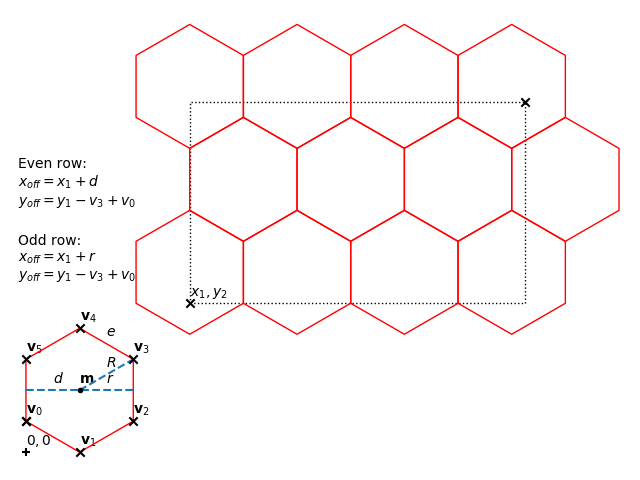
\includegraphics[scale=.7]{img/hexagons}
			\caption[Hexagon tessellation]{\textbf{Hexagon tessellation:} Located at the left bottom corner in red a hexagon defined by its geometric properties the 6 vertex vectors \{$\vec{v_0},...,\vec{v_5}$\} (black crosses), with center vector $\vec{m}$, edge length $e$, $R$ radius of the circumscribing circle, $r$ radius of the inscribed circle and $d$ the length of the short diagonal. Top right black dotted box are the bounds of an area which is tessellated by a hexagon grid in red. Each grid cell is translated from the origin hexagon at its position by computing the $x_{off}$ and $y_{off}$ offset with the presented equations at the left-hand side of the grid. }
			\label{fig:hexagon}
		\end{figure}
		% TODO DESCRIBE THE BINNING OF DATA AND WHAT WE WANT TO ACHIEVE
		Binning of raster data is easy we just have a point in polygon problem each points/pixels falling in hexagon are counted and aggregated through a function. In case of drivers of deforestation we count all driver classes per hexagon and compute ratios next we compute the sha \note{describe for each map how you build it}
		% TODO DESCRIBE CLIPPING
		As mentioned before for the visualization of the drivers of deforestation map we want to segment the hexagons with horizontal lines and each segment should represent the share of the direct deforestation driver within the tessellated area. To compute the split line for a certain hexagon we need the hexagon R computeable from the area of the hexagon equation \ref{eq:radius} and the rectangular bounds of the hexagon. We compute the relative share of an deforestation driver per hexagon this relative share can be used to compute the y-axis coordinate of an split line equation \ref{eq:percentage}. A regular hexagon can not only be presented in it vertex form as shown above. We can also use functions to define the hexagon shape. A hexagon consist of 2 picewise functions where each function consist of 3 linear functions restricted to an intervall. If we invert these functions we can use these functions to compute the x-coordinate of the split line with the previous computed y-coordinate Equations \ref{eq:left} and \ref{eq:right}. As a results we receive the solution matrix L which represents the horizontal line segment splitting the hexagon at the point where we want (driver ratio share) equation \ref{eq:line}. The solution matrix can be plugged in to a polygon split function which separates the hexagon polygon in a upper and lower part to do so we iterate over the hexagon vertices and decide if they are above or under the split line and append to a lower upper polygon. These list are our results \note{explain better split function}.
		\begin{equation}
		\label{eq:radius}
			R = \frac{\sqrt{2A}}{\sqrt[4]{27}}
		\end{equation}
		\begin{equation}
		\label{eq:percentage}
			y = \frac{P(y_2-y_1)}{100} + y_1
		\end{equation}
		\begin{equation}
		\label{eq:left}
			f^{-1}(y) =
			\begin{cases} 
				-\frac{y - y_1}{\tan{(\frac{\pi}{6}})} + \frac{x_1 + x_2}{2} & \text{if } y_1 \le y < y_1 + R\sin{(\frac{5\pi}{6})} \\
				x_1 & \text{if } y_1 + R\sin{(\frac{5\pi}{6})} \le y < R(\sin{(\frac{5\pi}{6})} + 1) \\
				\frac{y - y_2}{\tan{(\frac{\pi}{6}})} + \frac{x_1 + x_2}{2} & \text{if } R(\sin{(\frac{5\pi}{6})} + 1) \le y \le y_2
			\end{cases}
		\end{equation}
		\begin{equation}
		\label{eq:right}
			g^{-1}(y) = 
			\begin{cases} 
				\frac{y - y_1}{\tan{(\frac{\pi}{6}})} + \frac{x_1 + x_2}{2} & \text{if } y_1 \le y < y_1 + R\sin{(\frac{5\pi}{6})} \\
				x_2 & \text{if } y_1 + R\sin{(\frac{5\pi}{6})} \le y < R(\sin{(\frac{5\pi}{6})} + 1) \\
				-\frac{y - y_2}{\tan{(\frac{\pi}{6}})} + \frac{x_1 + x_2}{2} & \text{if } R(\sin{(\frac{5\pi}{6})} + 1) \le y \le y_2
			\end{cases}
		\end{equation}
		\begin{equation}
		\label{eq:line}
			\mathbf{L} =
			\begin{bmatrix}
				f^{-1}(y) & g^{-1}(y) \\
				y & y
			\end{bmatrix}
		\end{equation}

	\newpage
		\chapter{Results}
\label{ch:results}
	\note{IN PROGRESS}

	\section{Deforestation}
	\label{sec:results_deforestation}

		\subsection{Forest definition}
		\label{subsec:results_forest_definition}
		%TODO appendix graph distribution of the similarity indexes
		%TODO review
			\note{Goal (review):} Our goal was to determine at which canopy cover class the similarity between both layers is greatest to get the subsequent proximate deforestation driver for stable land cover changes optimal by anthropogenic causes by keeping the largest number of pixels from the gfc dataset. We applied the jaccard index for searching the similarity. We grouped our analysis by continental regions americas, asia, africa. Americas accounts for 82 tiles, Asia 86 tiles and Africa 101. We excluded from the analysis all tiles where the initial jaccard index is zero because theses tiles does not contain any tree cover in both tile pairs. This results in 76 Americas , 73 asia and 86 africa. Further we determined the optimal canopy density class for all regions and for single regions by applying the non parametric two and one sided wilcoxon signed rank test. Our initial hypothesis was that the agreement is max between gl30 and hansen when the selected canopy density is between 30 and 100. Because then both datasets should agree by their authors definition of tree cover. The following paragraphs present the results of the analysis for each continental region. 

			\note{Americas (review):} Figure \ref{fig:jaccard} shows the quartile distribution of the computed jaccard index for each tile pair for each canopy density class over the three continental regions. Plotted on the x-axis is the canopy density class identifier where $JI_0$ accounts for (0,100], $JI_0$ (10,100], $JI_0$ (20,100], and $JI_0$ (30,100]. The y-axis is the corresponding jaccard index between 0 and 1 for the corresponding tile pair where 1 means total agreement and 0 total disagreement. The sample mean highlight by red crosses in the boxplot for the Americas does not change significantly within the different canopy density classes. For all experiments it is approximately 0.62. While the sample median decreases from 0.68 to 0.66 from the first canopy density class the last canopy density class. For the first canopy class the upper 25 \% of the samples have tree cover similarity ranging between approximately 0.8 and 1.0. This behavior can be observed at the other canopy density classes to only the maximal similarity increases slightly from 0.9787 to 0.9798. As the figure \note{appendix} suggests the change of the canopy density have only little impact on the tiles where already the similarity is high for the upper 25 percent. The similarity range of the first two canopy density classes for the lower 25 percent of the samples ranges between approximately 0.0003 and 0.47. Whereas the range for last to canopy classes ranges between 0.0 and 0.5. This suggests that the exclusion of higher canopy densities decreases the similarity at samples where the similarity is already low also shown in figure \note{appendix}. 50 percent of the samples have a jaccard index between approximately 0.5 and 0.8 where here the highest mobility of similarity increase and decrease can be observed. To deduce which canopy density class yield the highest similarity in the distribution overall all samples from americas we applied a wilcoxon test. Tabel \ref{tab:wilcoxontwosided_regions} and \ref{tab:wilcoxontwosided_regions} shows the results from these tests. The two sided test reveals that only the similarity distribution between $JI_0$ and $JI_1$ has a significant (p<0.01) difference in distribution. The other Jaccard Index pairs show now significant difference in distribution. The tree cover similarity distribution of $JC_1$ is significantly greater than $JC_0$ (p<0.005) as the results from the one sided test show in the second table. Therefore the exclusion of canopy densities < 11 fosters the overall agreement between both tree cover datasets. Further the test also reveals that the similarity distribution of $JC_2$ is significantly greater than $JC_1$ (p<0.05) but by the comparison of $JC_1$ and $JC_2$ shows no clear trend in a certain direction. It is to assume that $JC_2$ improves only the tree cover agreement for certain tile pairs and not in general. The same accounts for $JC_3$. For studies targeting Americas it is to recommended to use from the Global Forest Change dataset data which lays within the canopy densities greater than 10 percent.
			\begin{figure}[ht]
				\centering
				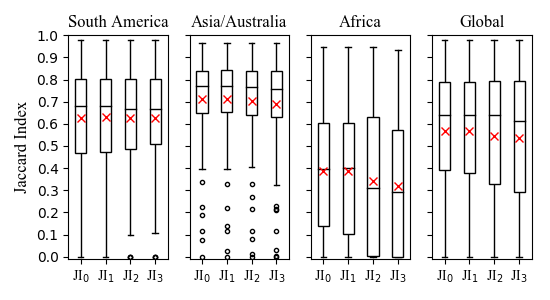
\includegraphics[scale=.91]{img/jaccard}
				\caption[Tree cover similarity distribution of the continental regions]{\textbf{Tree cover similarity distribution over the continental regions:} This boxplot shows the distribution of computed Jaccard Index for each raster image tile pair of GlobeLand30 and Global Forest Change tree cover from 2000. The labels $JI_0$, $JI_1$, $JI_2$, and $JI_3$ on the x-axis account for the canopy density classes (0,100], (10,100], (20,100], and (30,100], respectively. The y-axis is the computed Jaccard Index for the corresponding raster image pair, where 0 is a total disagreement and 1 a total agreement. Red crosses within the $Q_{25}$, $Q_{50}$, and $Q_{75}$ boxes highlight the sample mean. Whiskers are 1.5 times the $IQR$.}
				\label{fig:jaccard}
			\end{figure}
			\begin{table}[ht]
				\centering
				\caption[Regional two-sided Wilcoxon signed-rank test]{\textbf{Regional two-sided Wilcoxon signed-rank test:} This table shows, regional differences in the tree cover agreement by considering different canopy densities between GlobeLand30 and Global Forest Change at 2000. The classes $JI_0$, $JI_1$, $JI_2$, and $JI_3$ as row and column headings account for the canopy density classes (0,100], (10,100], (20,100], and (30,100], respectively. The test hypothesis is H$_0$: $X_1=X_2$ where $X_1$ is the column $JI_n$ class and $X_2$ the row $JI_n$ class. The significance is indicated by $p^{*}<0.05$, $p^{**}<0.02$, and $p^{***}<0.01$.}
				\label{tab:wilcoxontwosided_regions}
				\begin{tabular}{llllllllll}
					\hline
					& \multicolumn{3}{|c}{Americas} & \multicolumn{3}{|c|}{Asia} & \multicolumn{3}{c|}{Africa} \\
					Cls & JI$_0$ & JI$_1$ & JI$_2$ & JI$_0$ & JI$_1$ & JI$_2$ & JI$_0$ & JI$_1$ & JI$_2$ \\\hline
					JI$_0$ & - & - & - & - & - & - & - & - & - \\
					JI$_1$ & .00$^{***}$ & - & - & .72 & - & - & .22 & - & - \\
					JI$_2$ & .06 & .36 & - & .00$^{***}$ & .00$^{***}$ & - & .03$^{*}$ & .03$^{*}$  & - \\
					JI$_3$ & .16 & .50 & .60 & .00$^{***}$ & .00$^{***}$ & .00$^{***}$ & .00$^{***}$ & .00$^{***}$ & .00$^{***}$ \\\hline
				\end{tabular}
			\end{table}
			\begin{table}[ht]
				\centering
				\caption[Regional one-sided Wilcoxon signed-rank test]{\textbf{Regional one-sided Wilcoxon signed-rank test:} This table shows, the direction of regional differences in the tree cover agreement by considering different canopy densities between GlobeLand30 and Global Forest Change at 2000. The classes $JI_0$, $JI_1$, $JI_2$, and $JI_3$ as row and column headings account for the canopy density classes (0,100], (10,100], (20,100], and (30,100], respectively. The test hypothesis is H$_0$: $X_1\leq X_2$ and H$_0$: $X_2\geq X_1$ where $X_1$ is the column $JI_n$ class and $X_2$ the row $JI_n$ class. The significance is indicated by $p^{*}<0.05$, $p^{**}<0.025$, $p^{***}<0.01$, and $p^{\dagger}<0.005$.}
				\label{tab:wilcoxononesided_regions}
				\begin{tabular}{lllllllllllll}
					\hline
					& \multicolumn{4}{|c}{Americas} & \multicolumn{4}{|c|}{Asia} & \multicolumn{4}{c|}{Africa} \\
					Cls & JI$_0$ & JI$_1$ & JI$_2$ & JI$_3$ & JI$_0$ & JI$_1$ & JI$_2$ & JI$_3$ & JI$_0$ & JI$_1$ & JI$_2$ & JI$_3$ \\\hline
					JI$_0$ & - & .00$^{\dagger}$ & .03$^{*}$ & .08 & - & .64 & 1. & 1. & - & .11 & .98 & 1. \\
					JI$_1$ & 1. & - & .18 & .25 & .36 & - & 1. & 1. & .89 & - & .99 & 1. \\
					JI$_2$ & .97 & .82 & - & .30 & .00$^{\dagger}$ & .00$^{\dagger}$ & - & 1. & .02$^{**}$ & .01$^{**}$ & - & 1. \\
					JI$_3$ & .92 & .75 & .70 & - & .00$^{\dagger}$ & .00$^{\dagger}$ & .00$^{\dagger}$ & - & .00$^{\dagger}$ & .00$^{\dagger}$ & .00$^{\dagger}$ & - \\\hline
				\end{tabular}
			\end{table}
 
			\note{Asia (review):} As figure \ref{fig:jaccard} suggest does the sample mean is approximately 0.7 for all canopy classes in asia. It decreases slightly at higher canopy density intervals. The median is approximately 0.8 by showing also a slight decrease when the canopy density class is raised. The similarity of the upper 25 percent of the samples is approximately 0.85 and 0.96 and the maximum similarity decreases slightly from 0.9654 to 0.9634 by increasing canopy density interval. This suggests as the appendix figure shows that high ranking tiles are not largely impacted by changes in the canopy density. For Asia the range of the lower 25 percent of the samples is quite large. It ranges between approximately 0.65 and 0.0 and as appendix shows the mobility of the samples show an overall downward trend. The iqr for the first two canopy density classes ranges between 0.65 and 0.85. The exclusion of lower canopy densities have not an large impact on the distribution of tree cover similarity. For last two canopy density classes the range between q1 and q3 is increasing. The exclusion of higher canopy densities leads to overall downwards trend within this intervals figure appendix. For asia the two sided wilcoxon test in table \ref{tab:wilcoxontwosided_regions} reveals that the similarity distribution between every sample pair is significantly different (p<0.01) except the pair of $JI_1$ and $JI_0$. The directional test in table \ref{tab:wilcoxononesided_regions} shows that the overall tree cover agreement of $JI_2$ and $JI_3$ is significantly smaller than $JI_0$ and $JI_1$ (p<0.005). The direction of distribution differences between $JC_0$ and $JC_1$ is not clearly deduce able. This could be explained over a large variability within regional tree cover agreement also a clearer picture could be achieved by applying smaller canopy density exclusion stepping. For studies in asia it is to recommended to use from the Global Forest Change dataset data which lays within the canopy densities greater than 10 percent or the entire data range. Here it must be decided if moving the canopy density threshold below the GlobaLand30 forest cover definition is a good trade for increased sample size.

			\note{Africa (review):} As figure \ref{fig:jaccard} for Africa suggests is the similarity distribution mobility of the samples in Africa at highest. The first two similarity distributions have an comparable mean and median at 0.38 and 0.4. The last two classes show a strong decline in mean and median to approximately 0.33 and 0.3. The mobility of the upper 25 percent of the first two canopy density classes is already quite strong as figure appendix suggests. While the iqr range for $JI_0$ is between 0.15 and 0.6 the range increases for the second $JI_1$ by connecting to more agreement downwards trend. The tile pairs in africa are characterized by 17 (approx. 20 percent) where the tree cover agreement is smaller than 0.1. 11 of these tiles have already a agreement of 0.0 when the first canopy density is excluded. These trend continues as more canopy density is excluded as more samples have a agreement of 0.0. This explains the high iqr range for the canopy densities exclusion greater than 10 percent. At $JI_3$ already two fifth (42 percent) of the samples have an tree cover agreement lower than 0.1. The two sided wilcoxon test shows that the distribution of $JI_2$ and $JI_3$ significantly differs (p<0.05 and p<0.01). As the table suggest is the distribution of $JI_0$ and $JI_1$ nearly the same. The one sided test reveals that reducing the canopy density below 10 percent decreases the tree cover agreement between sample distributions. For $JI_0$ and the $JI_1$ the test reveals that no clear trend is detectable. Appendix figure shows that some samples benefit from the exclusion of canopy density and as mentioned some samples show a strong decrease in tree cover similarity. As the data shows is the regional dependency of tree cover agreement at largest. To maximize the similarity on continental level for africa it should the entire data range of Global Forest Change should be slected. It could also be also a solution to select canopy densities in the interval 10 to 100 but here the trade is to have tiles where no tree cover agreement is detectable.

			\note{Comparison between regions (review):} Table appendix shows that Asia has the highest tree cover similarity distribution over all regions within all tested canopy classes followed by the Americas for GlobeLand30 and Hansen 2000. Africa has the poorest tree cover agreement within our tested regions. As discussed in the previous paragraphs the reason could be that Americas and Asia have mainly core tropical forest zones where the forest cover is dense and the canopy density is above 30 percent. This can be highlighted by section tropical deforestation and the shown tree cover maps. Africa in comparison to Asia and Americas has large zones where the tree cover is high but the canopy density is low also described by the term sparse woodland. As it looks these sparse woodlands compete the forest detection methods of both datasets. This fact could lead within the hansen dataset to ghost deforestation because it is hard to detect sparse woodland it could be the annual deforestation does not detect it as forest and it is recognized as deforestation. Therefore in africa the rationality of tree cover agreement must be considered during preparation and validation of studies. Also it is to suggest to optimize tree cover agreement on regional scale and not over the entire continent. Overall regions the upper 25 percent of the samples benefit or shown only small changes if the canopy density is increased.

			\note{All regions (review):} To deduce in which canopy density interval we use the Global Forest Change data for our global study on proximate deforestation driver we analyzed the change of tree cover agreement over all samples. Figure \ref{fig:jaccard} shows on the right hand side of the image the distribution of tree cover agreement over the entire sample range. The mean and median shown only a slight decline overall canopy density test classes. As deduced for the regions also on global scale the upper 25 percent commonly benefit or show no change if the canopy density is increased. As the figure shows is the range of them between 0.8 and 1.0. When the canopy density is increased the range of the mid 50 percent increases which highlights a more similarity downwards trend within this group. This downwards trend of the mid is connected with a decrease in the range of the lower 25 percent. The first canopy density class is between 0.4 and 0.0 and the last is between 0.3 ad 0.0. The distribution comparison in table \ref{tab:wilcoxontwosided_all} shows that each sample class has significant differences (p<0.02 and p<0.01) except $JI_0$ and $JI_2$ where the similarity distribution could be the same. Table \ref{tab:wilcoxononesided_all} shows the direction of the distribution differences. Globally the tree cover agreement is highest when we consider only pixels within the canopy density interval (10,100] as the table shows. The distributions of tree cover agreement of $JI_0$, $JI_2$, and $JI_3$ are all significantly smaller than $JI_1$ (p<0.005 and p<0.01). By knowing this we decided to proceed for our study only with data within this tree cover interval. Therefore we filtered forest loss and gain of Global Forest Change to lay in this interval and classified them subsequently by superimposing the GlobeLand30 land cover layer. The result of this process are shown in section \ref{subsec:results_proxy_deforestation_driver}.
			\begin{table}[ht]
				\centering
				\caption[Global two-sided Wilcoxon signed-rank test]{\textbf{Regional two-sided Wilcoxon signed-rank test:} This table shows, global differences in the tree cover agreement by considering different canopy densities between GlobeLand30 and Global Forest Change at 2000. The classes $JI_0$, $JI_1$, $JI_2$, and $JI_3$ as row and column headings account for the canopy density classes (0,100], (10,100], (20,100], and (30,100], respectively. The test hypothesis is H$_0$: $X_1=X_2$ where $X_1$ is the column $JI_n$ class and $X_2$ the row $JI_n$ class. The significance is indicated by $p^{*}<0.05$, $p^{**}<0.02$, and $p^{***}<0.01$.}
				\label{tab:wilcoxontwosided_all}
				\begin{tabular}{llll}
					\hline
					Cls & JI$_0$ & JI$_1$ & JI$_2$ \\\hline
					JI$_0$ & - & - & - \\
					JI$_1$ & .00$^{***}$ & - & - \\
					JI$_2$ & .08 & .02$^{**}$ & - \\
					JI$_3$ & .00$^{***}$ & .00$^{***}$ & .00$^{***}$ \\\hline
				\end{tabular}
			\end{table}
			\begin{table}[ht]
				\centering
				\caption[Global one-sided Wilcoxon signed-rank test]{\textbf{Global one-sided Wilcoxon signed-rank test:} This table shows, the direction of global differences in the tree cover agreement by considering different canopy densities between GlobeLand30 and Global Forest Change at 2000. The classes $JI_0$, $JI_1$, $JI_2$, and $JI_3$ as row and column headings account for the canopy density classes (0,100], (10,100], (20,100], and (30,100], respectively. The test hypothesis is H$_0$: $X_1\leq X_2$ and H$_0$: $X_2\geq X_1$ where $X_1$ is the column $JI_n$ class and $X_2$ the row $JI_n$ class. The significance is indicated by $p^{*}<0.05$, $p^{**}<0.025$, $p^{***}<0.01$, and $p^{\dagger}<0.005$.}
				\label{tab:wilcoxononesided_all}
				\begin{tabular}{lllll}
					\hline
					Cls & JI$_0$ & JI$_1$ & JI$_2$ & JI$_3$ \\\hline
					JI$_0$ & - & .00$^{****}$ & .96 & 1. \\
					JI$_1$ & 1. & - & .99 & 1. \\
					JI$_2$ & .04$^{*}$ & .01$^{***}$ & - & 1. \\
					JI$_3$ & .00$^{****}$ & .00$^{****}$ & .00$^{****}$ & - \\\hline
				\end{tabular}
			\end{table}

		\subsection{Tree cover and deforestation}
		\label{subsec:results_tree_cover_and_deforestation}
		%TODO images of loss and canopy
		\note{Goal:}
		\note{Americas:} \note{Asia:} \note{Africa:}

		\subsection{Proximate deforestation driver}
		\label{subsec:results_proxy_deforestation_driver}

		\subsection{Accuracy assessment}
		\label{subsec:results_accuracy_assessment}
		%TODO distribution is it in line with global estimates
			\note{Goal (review):} Goal is the assessment of the accuracy of our proximate deforestation driver predictions. We created a set of ground truth data by sampling our proximate deforestation driver layers. In each region we select per random 10 tiles and draw 200 samples per tile. The 200 samples comprises pixels over the full value range of our proximate deforestation driver classes. We imported the prepared sample to our JavaScript application and subsequently classified each sample with a label. To determine the accuracy we used a confusion matrix and the derived metrics like producers accuracy, overall accuracy, kappa coefficient etc.

			\note{Results (review):} Table \ref{tab:results_confusion_matrix} shows the confusion matrix to determine the accuracy of our predictions where the term reference refers to the labeling of pixel by our visual interpretation and predictions refer to the labeling of our proximate driver predictions. The abbreviations PAc, UAc, OvAc, Com, Om, Tot, and Kappa refer to the terms Producers-Accuracy, Users-Accuracy, Overall-Accuracy, Error of Commission, Error of Omission, row or column total, and Kappa Coefficient. From the 6000 samples we draw from our study extent 14 \%, 20 \%, 22 \%, 32 \%, 8 \%, 2 \%, 0.5 \%, 2 \%, and 0.5 \% account for cultivated land (10), tree cover (20), regrowth (25), shrubland (40), wetland (50), water (60), artificial land (80), and bareland (90), respectively. The method predicts a distribution of 15 \%, 18 \%, 27 \%, 31 \%, 7 \%, 1 \%, 0.8 \%, 1 \%, and 0.2 \% for the land cover classes 10, 20, 25, 30, 40, 50, 60, 80, and 90, respectively. Our method achieved an overall accuracy of approximately 76 \%

			\begin{itemize}
				\item grassland in majority with anthropogenic influence at many sides at water hole was detectable
				\item decision between regrowth and natural tree cover, relayed on expert knowledge how homogeneous is canopy
				\item shrub land comprises natural landscapes, young plantations, and areas for cattle ranching
				\item strong variability of images some high res some landsat quality
			\end{itemize}
			\begin{table}[ht]
				\centering
				\caption[Confussion matrix]{\textbf{Confussion matrix for accuracy assessment:} We draw 6000 samples from 10 random selected tiles from the three regions Americas, Asia and Africa. Labels refer to our proximate deforestation driver classes which correspond to GlobeLand30 classification schema in table \ref{tab:gl30_classes}. Reference refers to the samples we classified by visual interpretation of external imagery and predictions refer to the label the sample has in our proximate driver product. The abbreviations PAc, UAc, OvAc, Com, Om, Tot, and Kappa refer to the terms Producers-Accuracy, Users-Accuracy, Overall-Accuracy, Error of Commission, Error of Omission, row or column total, and Kappa Coefficient.}
				\label{tab:results_confusion_matrix}
				\begin{tabular}{llrrrrrrrrrrrr}
					\hline
					& & \multicolumn{9}{c}{Reference} & & & \\\cline{3-11}
					& Cls & 10 & 20 & 25 & 30 & 40 & 50 & 60 & 80 & 90 & Tot & UAc & Om \\\hline
					\multirow{9}{*}{\STAB{\rotatebox[origin=c]{90}{Prediction}}}
					& 10 & 730 & 37 & 62 & 15 & 16 & 2 & 3 & 5 & 0 & 870 & .84 & .16 \\ 
					& 20 & 41 & 744 & 56 & 189 & 31 & 12 & 0 & 15 & 4 & 1092 & .68 & .32 \\ 
					& 25 & 29 & 202 & 1155 & 172 & 22 & 10 & 5 & 11 & 4 & 1610 & .72 & .28 \\ 
					& 30 & 36 & 187 & 32 & 1466 & 73 & 21 & 0 & 17 & 0 & 1832 & .80 & .20 \\ 
					& 40 & 14 & 21 & 4 & 41 & 352 & 1 & 1 & 2 & 1 & 437 & .81 & .19 \\ 
					& 50 & 0 & 5 & 3 & 10 & 4 & 50 & 0 & 1 & 0 & 73 & .68 & .32 \\ 
					& 60 & 2 & 1 & 0 & 3 & 0 & 2 & 18 & 2 & 0 & 28 & .64 & .36 \\ 
					& 80 & 3 & 3 & 0 & 1 & 1 & 1 & 0 & 40 & 0 & 49 & .82 & .18 \\ 
					& 90 & 0 & 0 & 0 & 1 & 0 & 0 & 0 & 3 & 5 & 9 & .56 & .44 \\\hline 
					& Tot & 855 & 1200 & 1312 & 1898 & 499 & 99 & 27 & 96 & 14 & 6000 & & \\
					& PAc & .85 & .62 & .88 & .77 & .71 & .51 & .67 & .42 & .36 & Kappa & \multicolumn{2}{r}{OvAc} \\
					& Com & .15 & .38 & .12 & .23 & .29 & .49 & .33 & .58 & .64 & .69 & \multicolumn{2}{r}{.76} \\ \hline
				\end{tabular}
			\end{table}

	\section{Emissions}

	\section{Ecosystem service values}




%%%%%%% TABLE AND FIGURES

%			\begin{table}[ht]
%				\centering
%				\caption[Deforestation driver]{Absolute in km$^2$}
%				\label{tab:driver_tab}
%				\begin{tabular}{lcllrrr}
%					Class & Code & Type & & Americas & Asia & Africa \\\hline
%					\multirow{4}{*}{Agriculture} & \multirow{2}{*}{10} & \multirow{2}{*}{Cropland} & rel. & 24.37 & 18.37 & 25.01 \\
%					& & & abs. & 95908 & 38719 & 44368 \\
%					& \multirow{2}{*}{30} & \multirow{2}{*}{Grassland} & rel. & 46.19 & 8.41 & 50.46 \\
%					& & & abs. & 181781 & 17726 & 89516 \\
%					\multirow{4}{*}{Forestry/Plantations} & \multirow{2}{*}{25} & \multirow{2}{*}{Regrowth} & rel. & 14.40 & 70.27 & 18.61 \\
%					& & & abs. & 56671 & 148111 & 33014 \\
%					& \multirow{2}{*}{40} & \multirow{2}{*}{Shrubland} & rel. & 12.69 & 1.11 & 3.77 \\
%					& & & abs. & 49941 & 2340 & 6688 \\
%					\multirow{4}{*}{Urban/Mining} & \multirow{2}{*}{80} & \multirow{2}{*}{Artificial} & rel. & 0.41 & 0.46 & 0.71 \\
%					& & & abs. & 1614 & 970 & 1260 \\
%					& \multirow{2}{*}{90} & \multirow{2}{*}{Bareland} & rel. & 0.10 & 0.03 & 0.09 \\
%					& & & abs. & 394 & 63 & 160 \\
%					\multirow{4}{*}{Natural} & \multirow{2}{*}{50} & \multirow{2}{*}{Wetland} & rel. & 1.50 & 0.97 & 1.23 \\
%					& & & abs. & 5903 & 2045 & 2182 \\
%					& \multirow{2}{*}{60} & \multirow{2}{*}{Water} & rel. & 0.32 & 0.38 & 0.13 \\
%					& & & abs. & 1259 & 801 & 231 \\\hline
%					\multicolumn{3}{c}{\multirow{2}{*}{Forest loss}} & rel. & 3.87 & 4.68 & 1.69 \\
%					& & & abs. & 393550 & 210774 & 177400 \\
%					\multicolumn{3}{c}{Forest cover} & abs. & 10223187 & 4457940 & 10496591 \\\hline
%				\end{tabular}
%			\end{table}

% LATIN AMERICA
%			\begin{figure}[ht]
%				\centering
%				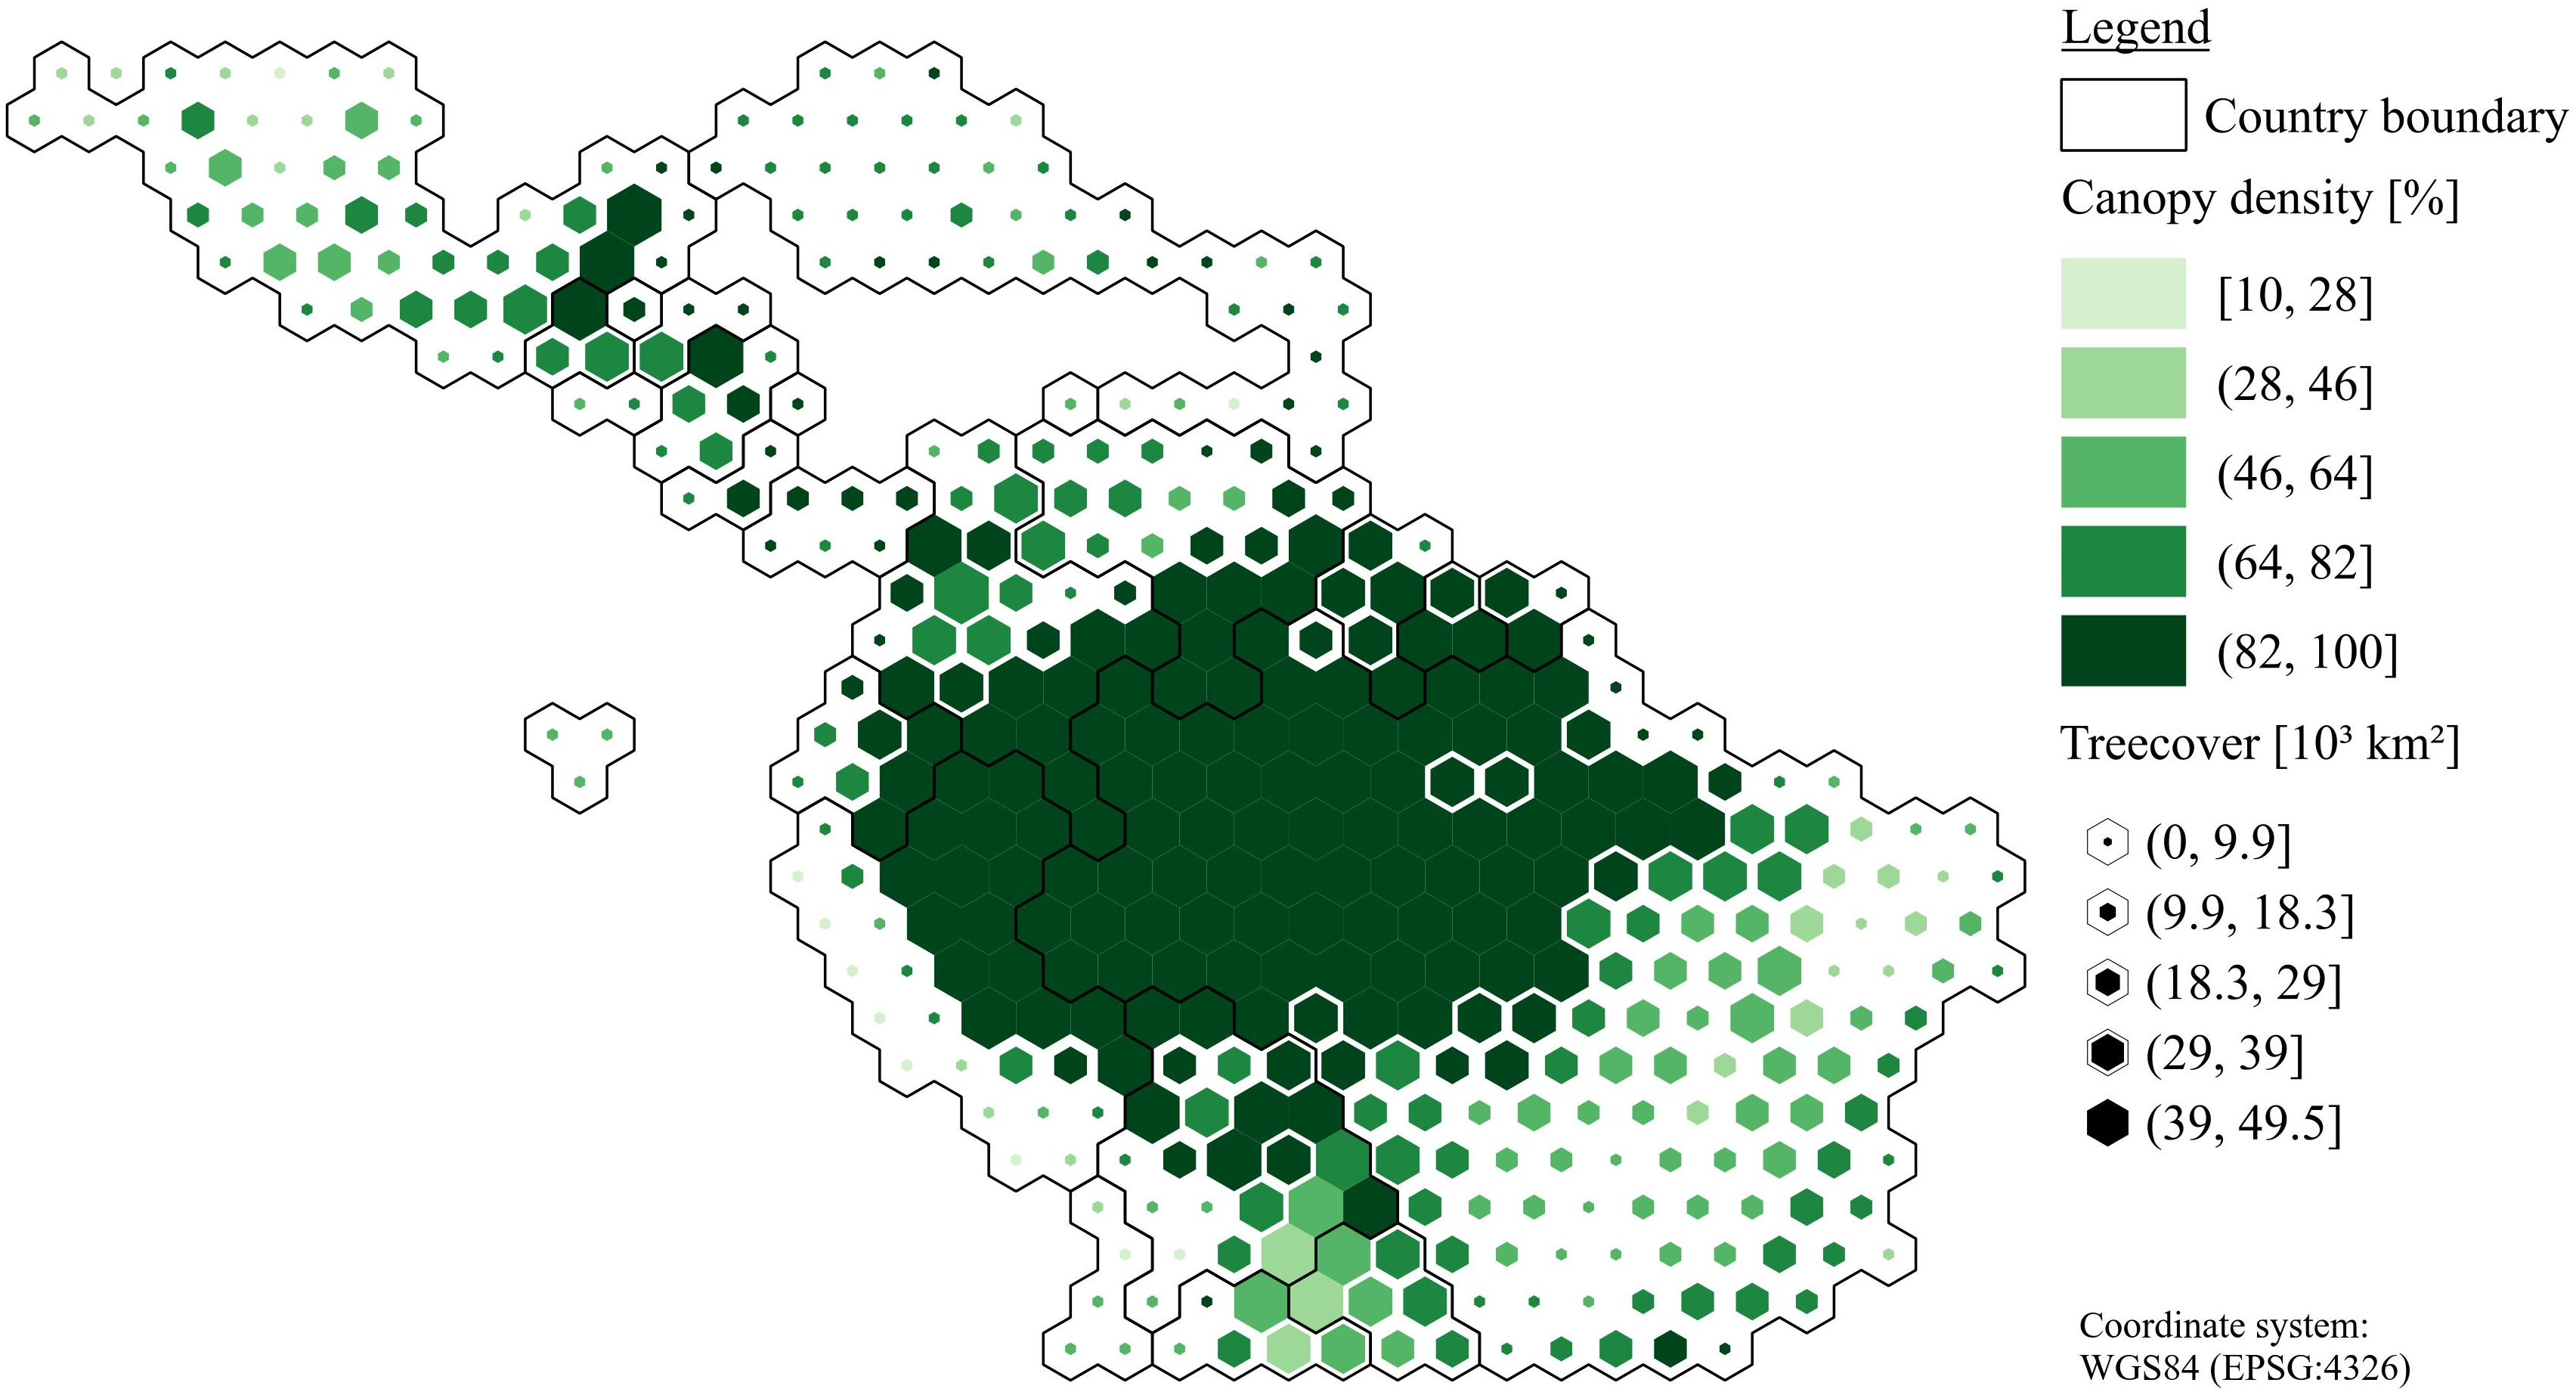
\includegraphics[scale=1]{img/americas_treecover_frameless}
%				\caption[Ecosystem service values]{}
%				\label{fig:americascover}
%			\end{figure}
%			\begin{figure}[ht]
%				\centering
%				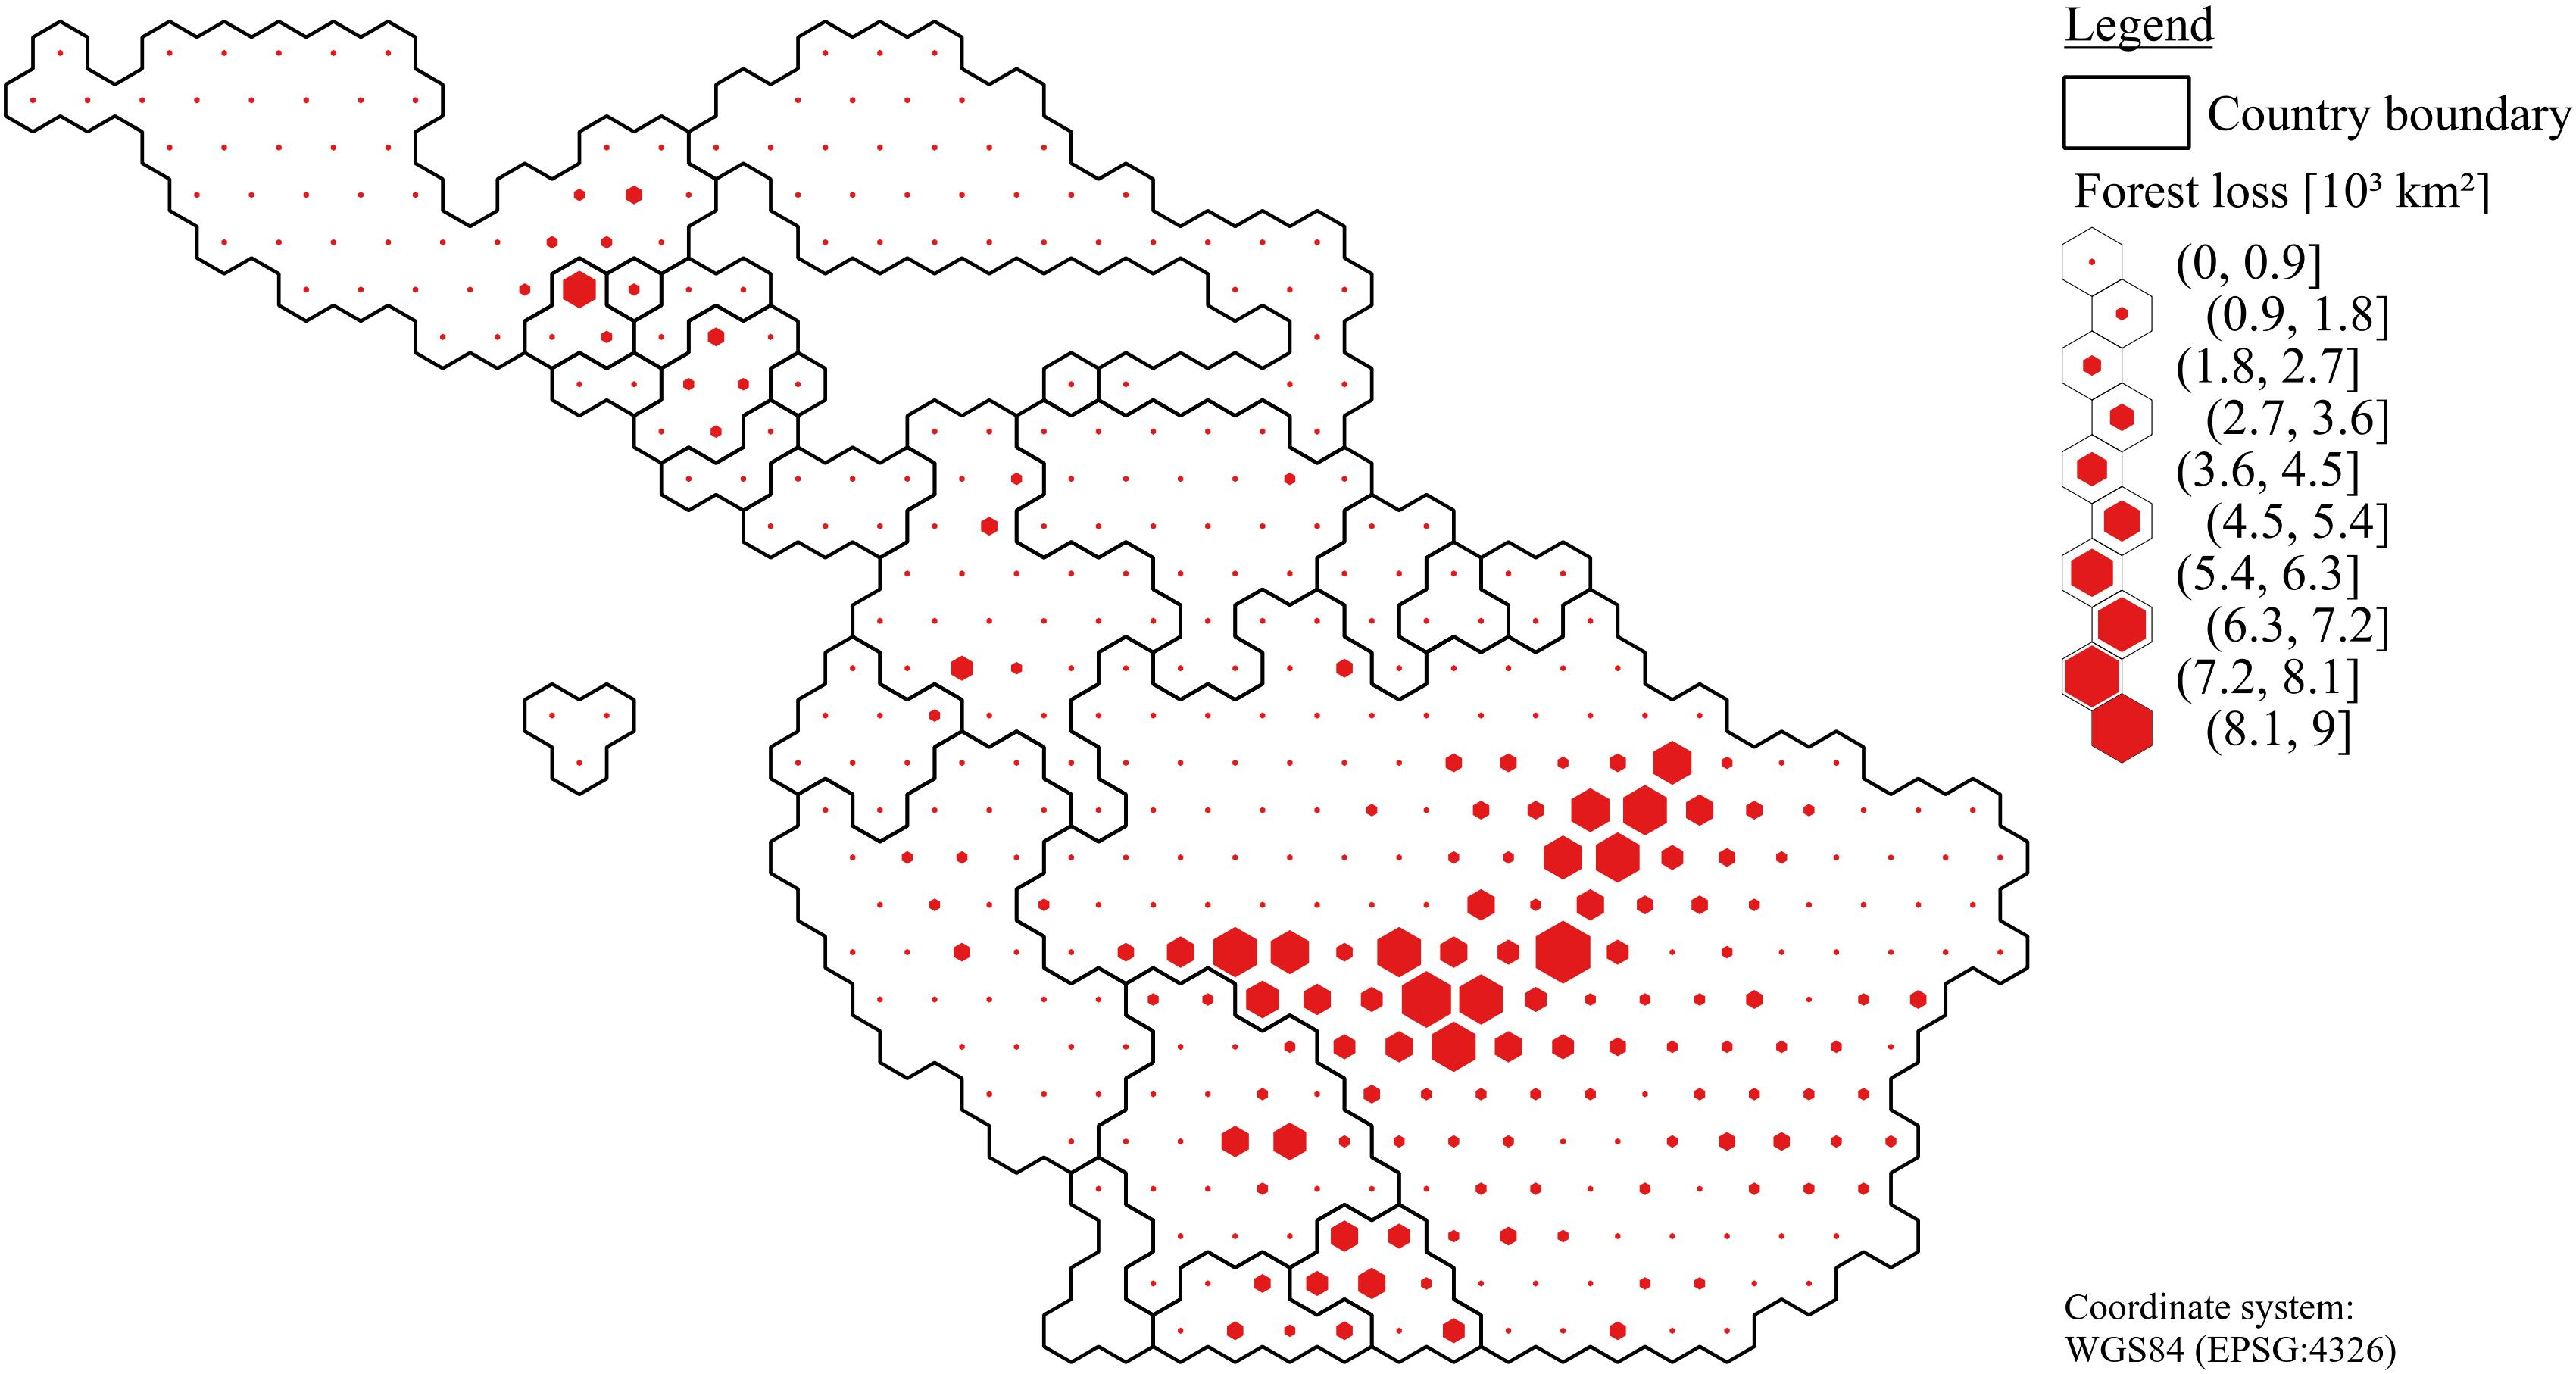
\includegraphics[scale=1]{img/americas_loss_frameless}
%				\caption[Ecosystem service values]{}
%				\label{fig:americasloss}
%			\end{figure}
%			\begin{figure}[ht]
%				\centering
%				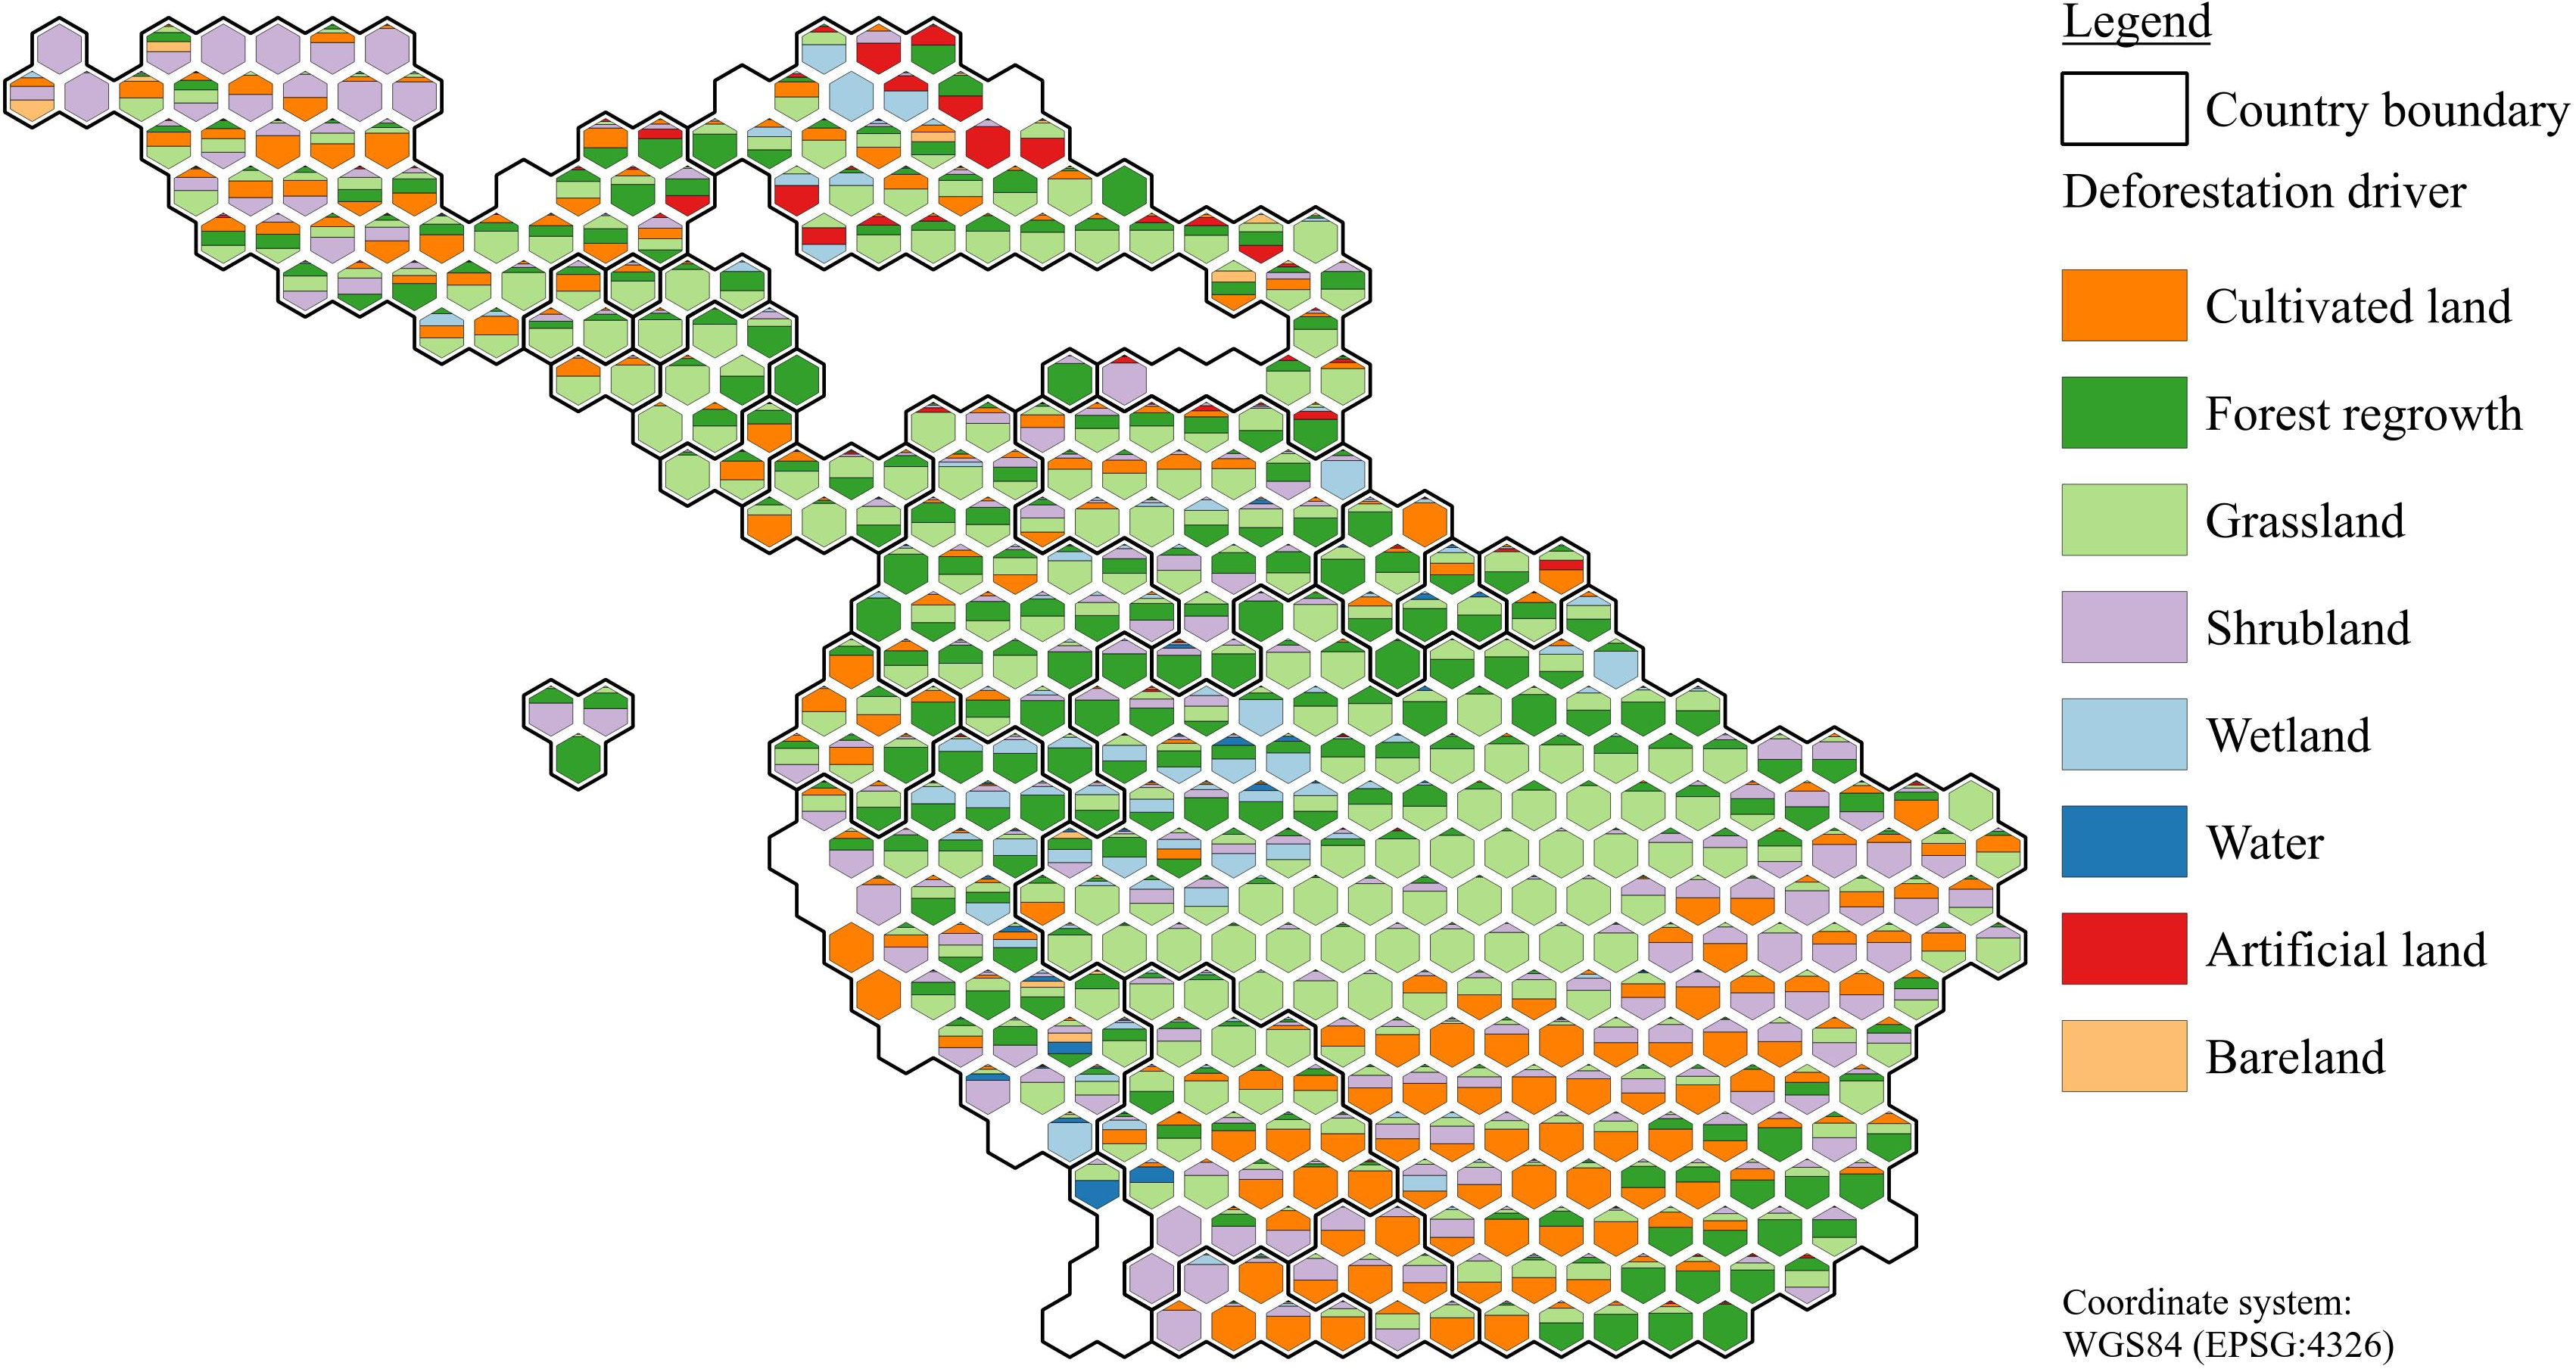
\includegraphics[scale=1]{img/americas_driver_frameless}
%				\caption[Ecosystem service values]{}
%				\label{fig:americasdriver}
%			\end{figure}

% ASIA
%			\begin{figure}[ht]
%				\centering
%				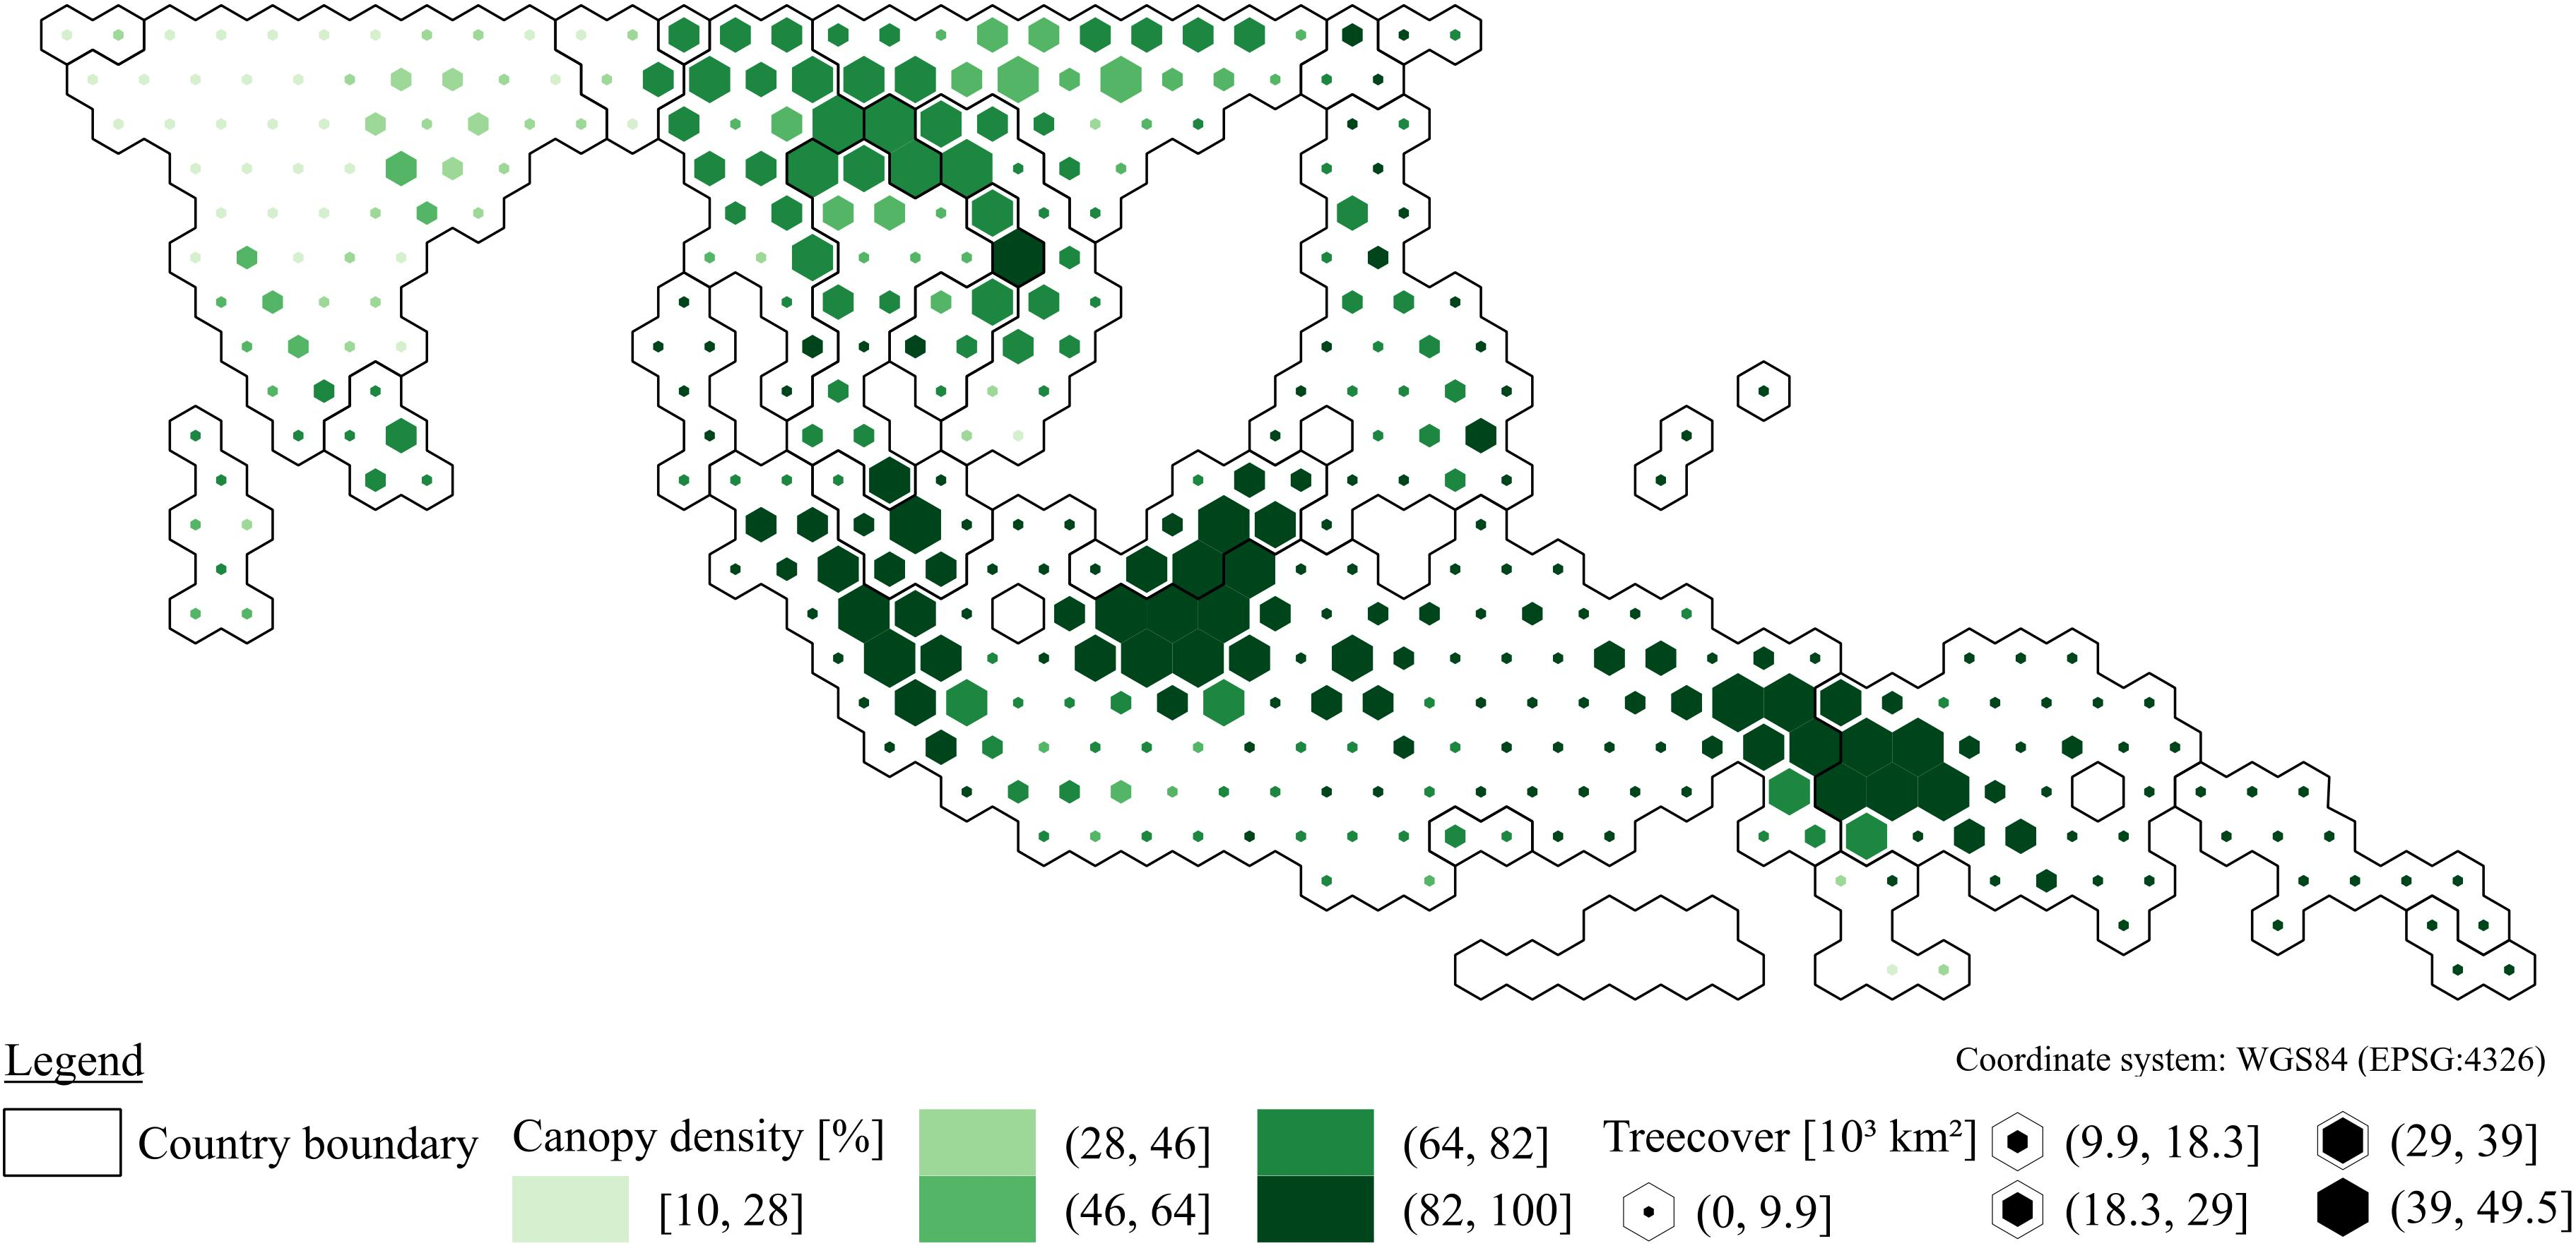
\includegraphics[scale=1]{img/asia_treecover_frameless}
%				\caption[Ecosystem service values]{}
%				\label{fig:asiacover}
%			\end{figure}
%			\begin{figure}[ht]
%				\centering
%				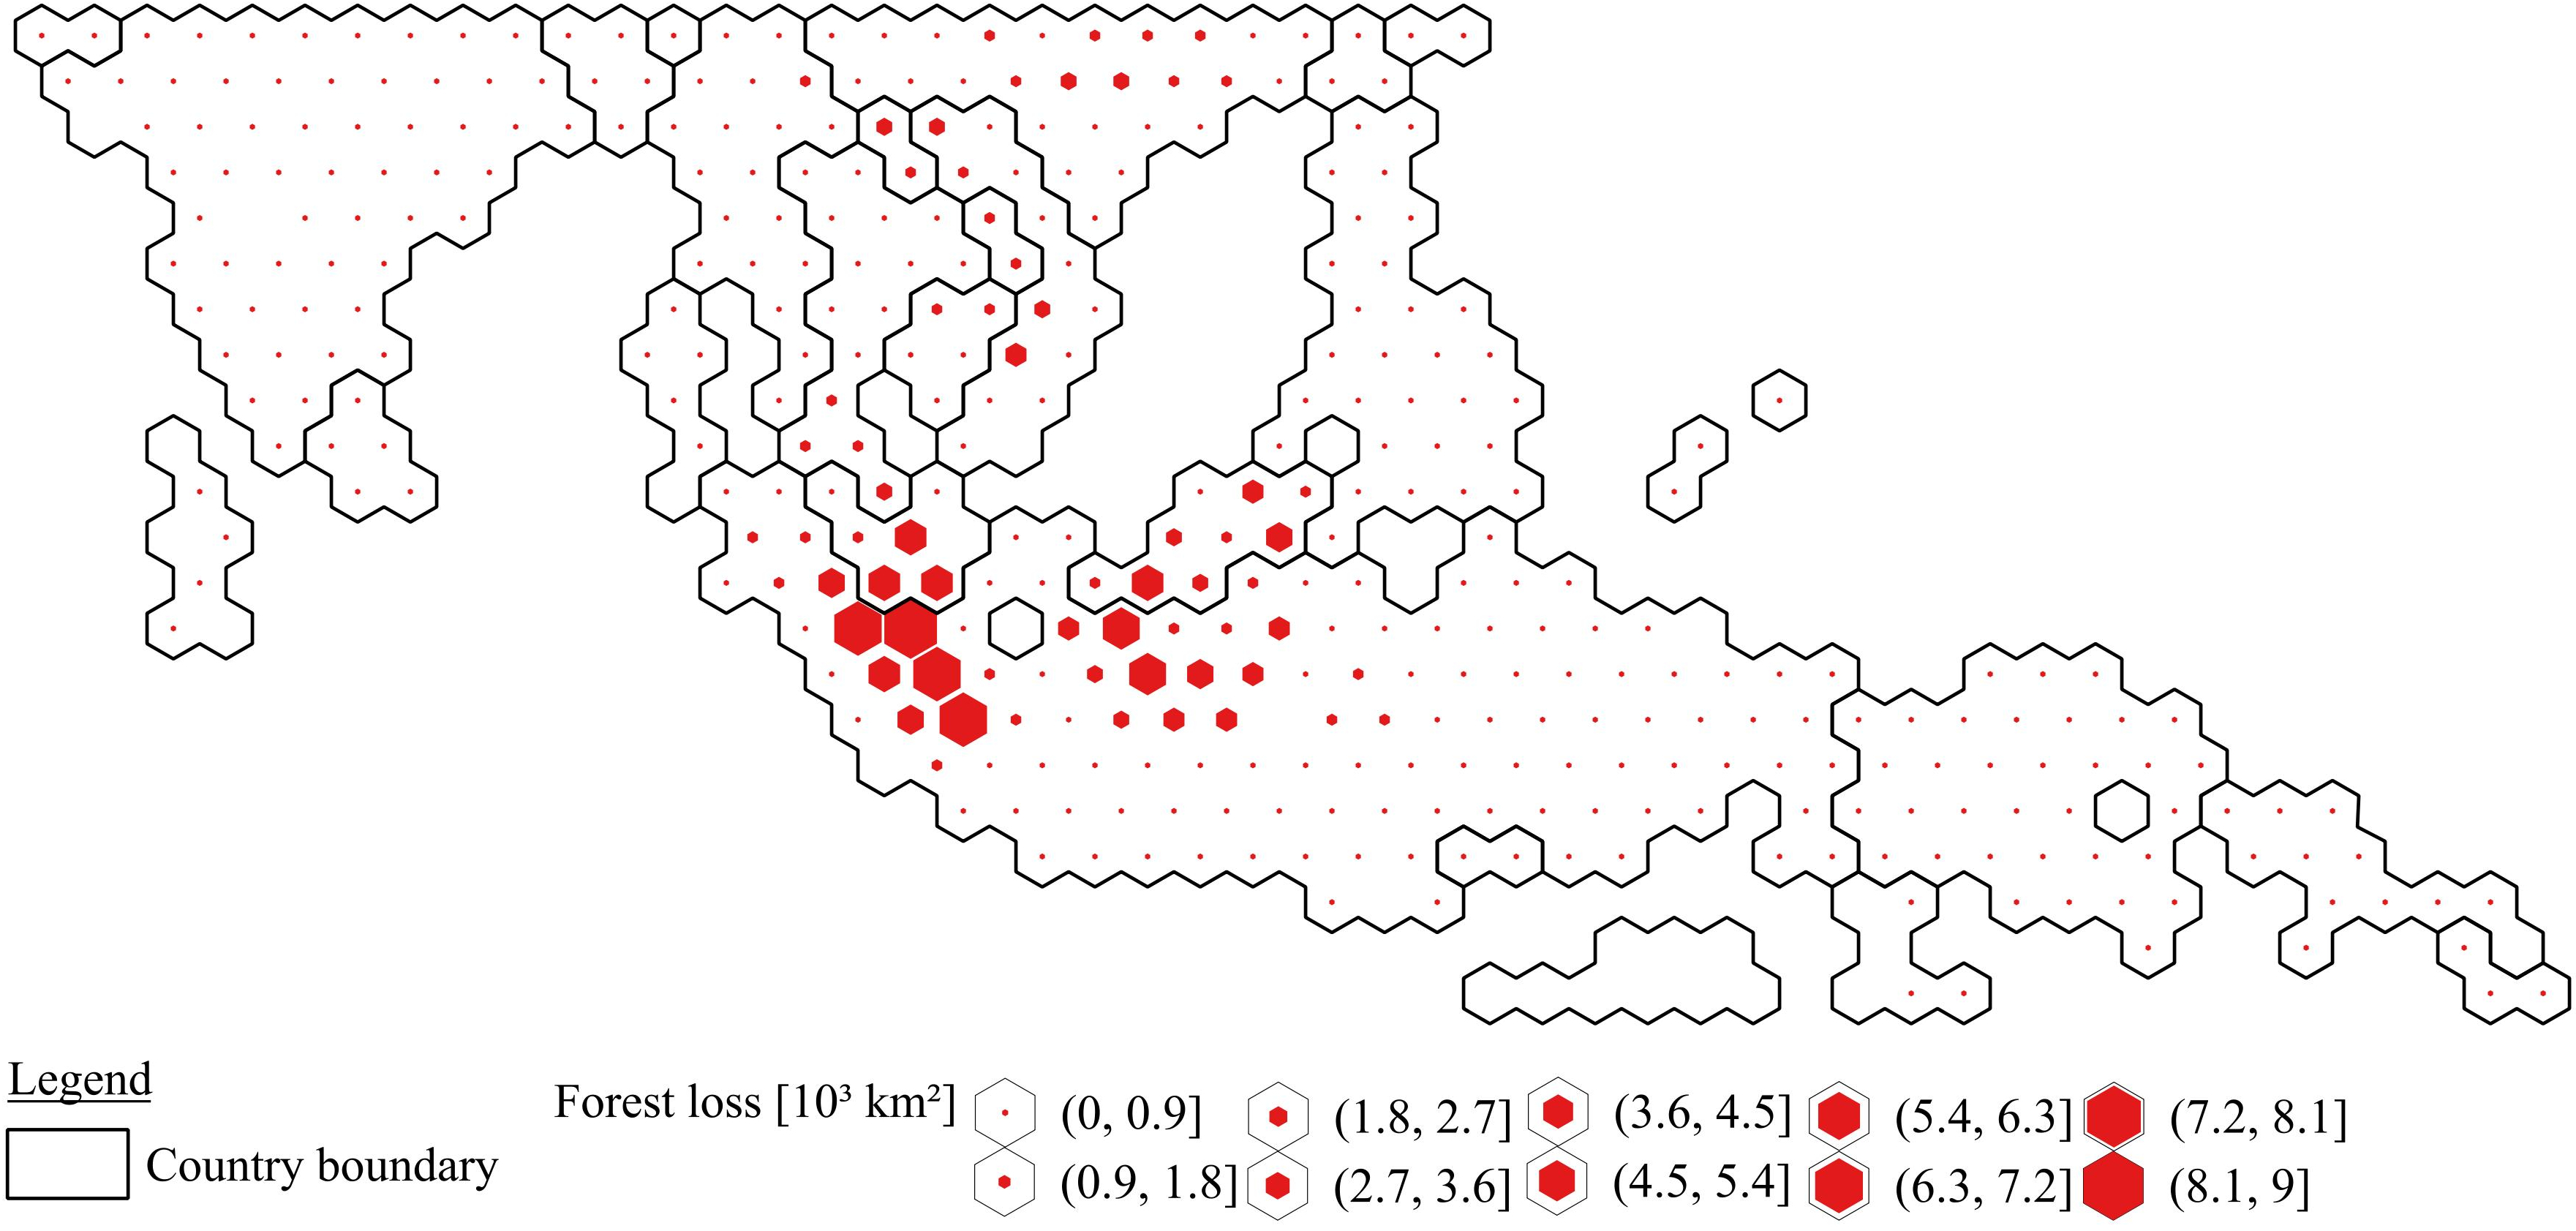
\includegraphics[scale=1]{img/asia_loss_frameless}
%				\caption[Ecosystem service values]{}
%				\label{fig:asialoss}
%			\end{figure}
%			\begin{figure}[ht]
%				\centering
%				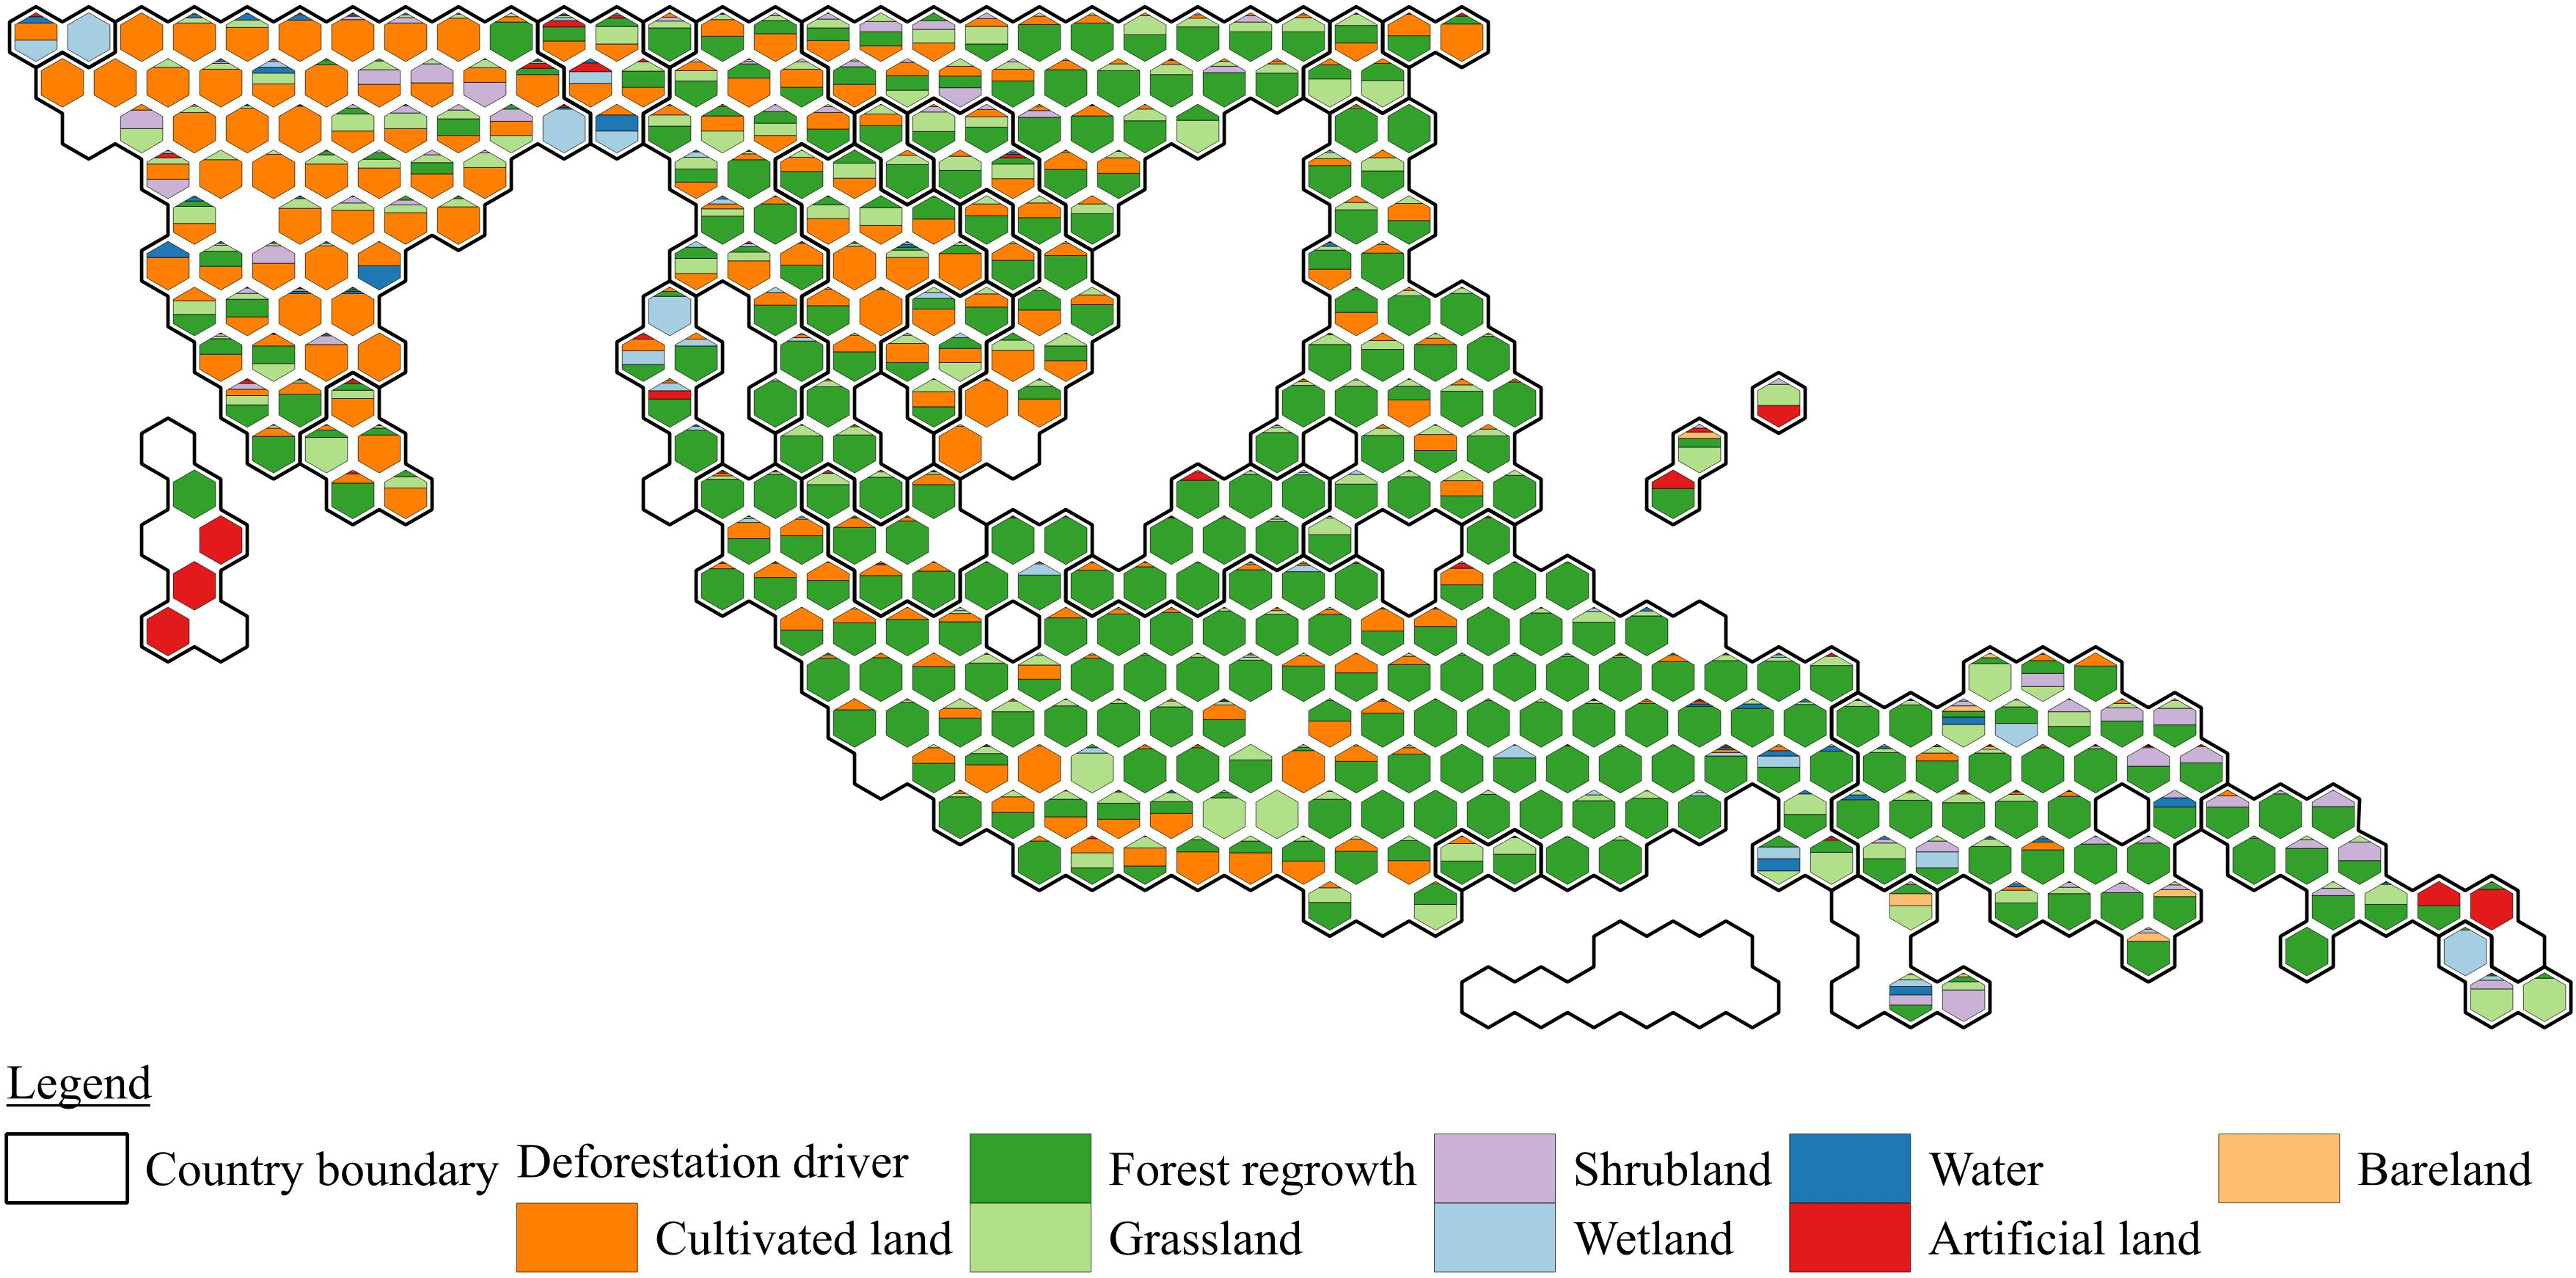
\includegraphics[scale=1]{img/asia_driver_frameless}
%				\caption[Ecosystem service values]{}
%				\label{fig:asiadriver}
%			\end{figure}

% AFRICA
%			\begin{figure}[ht]
%				\centering
%				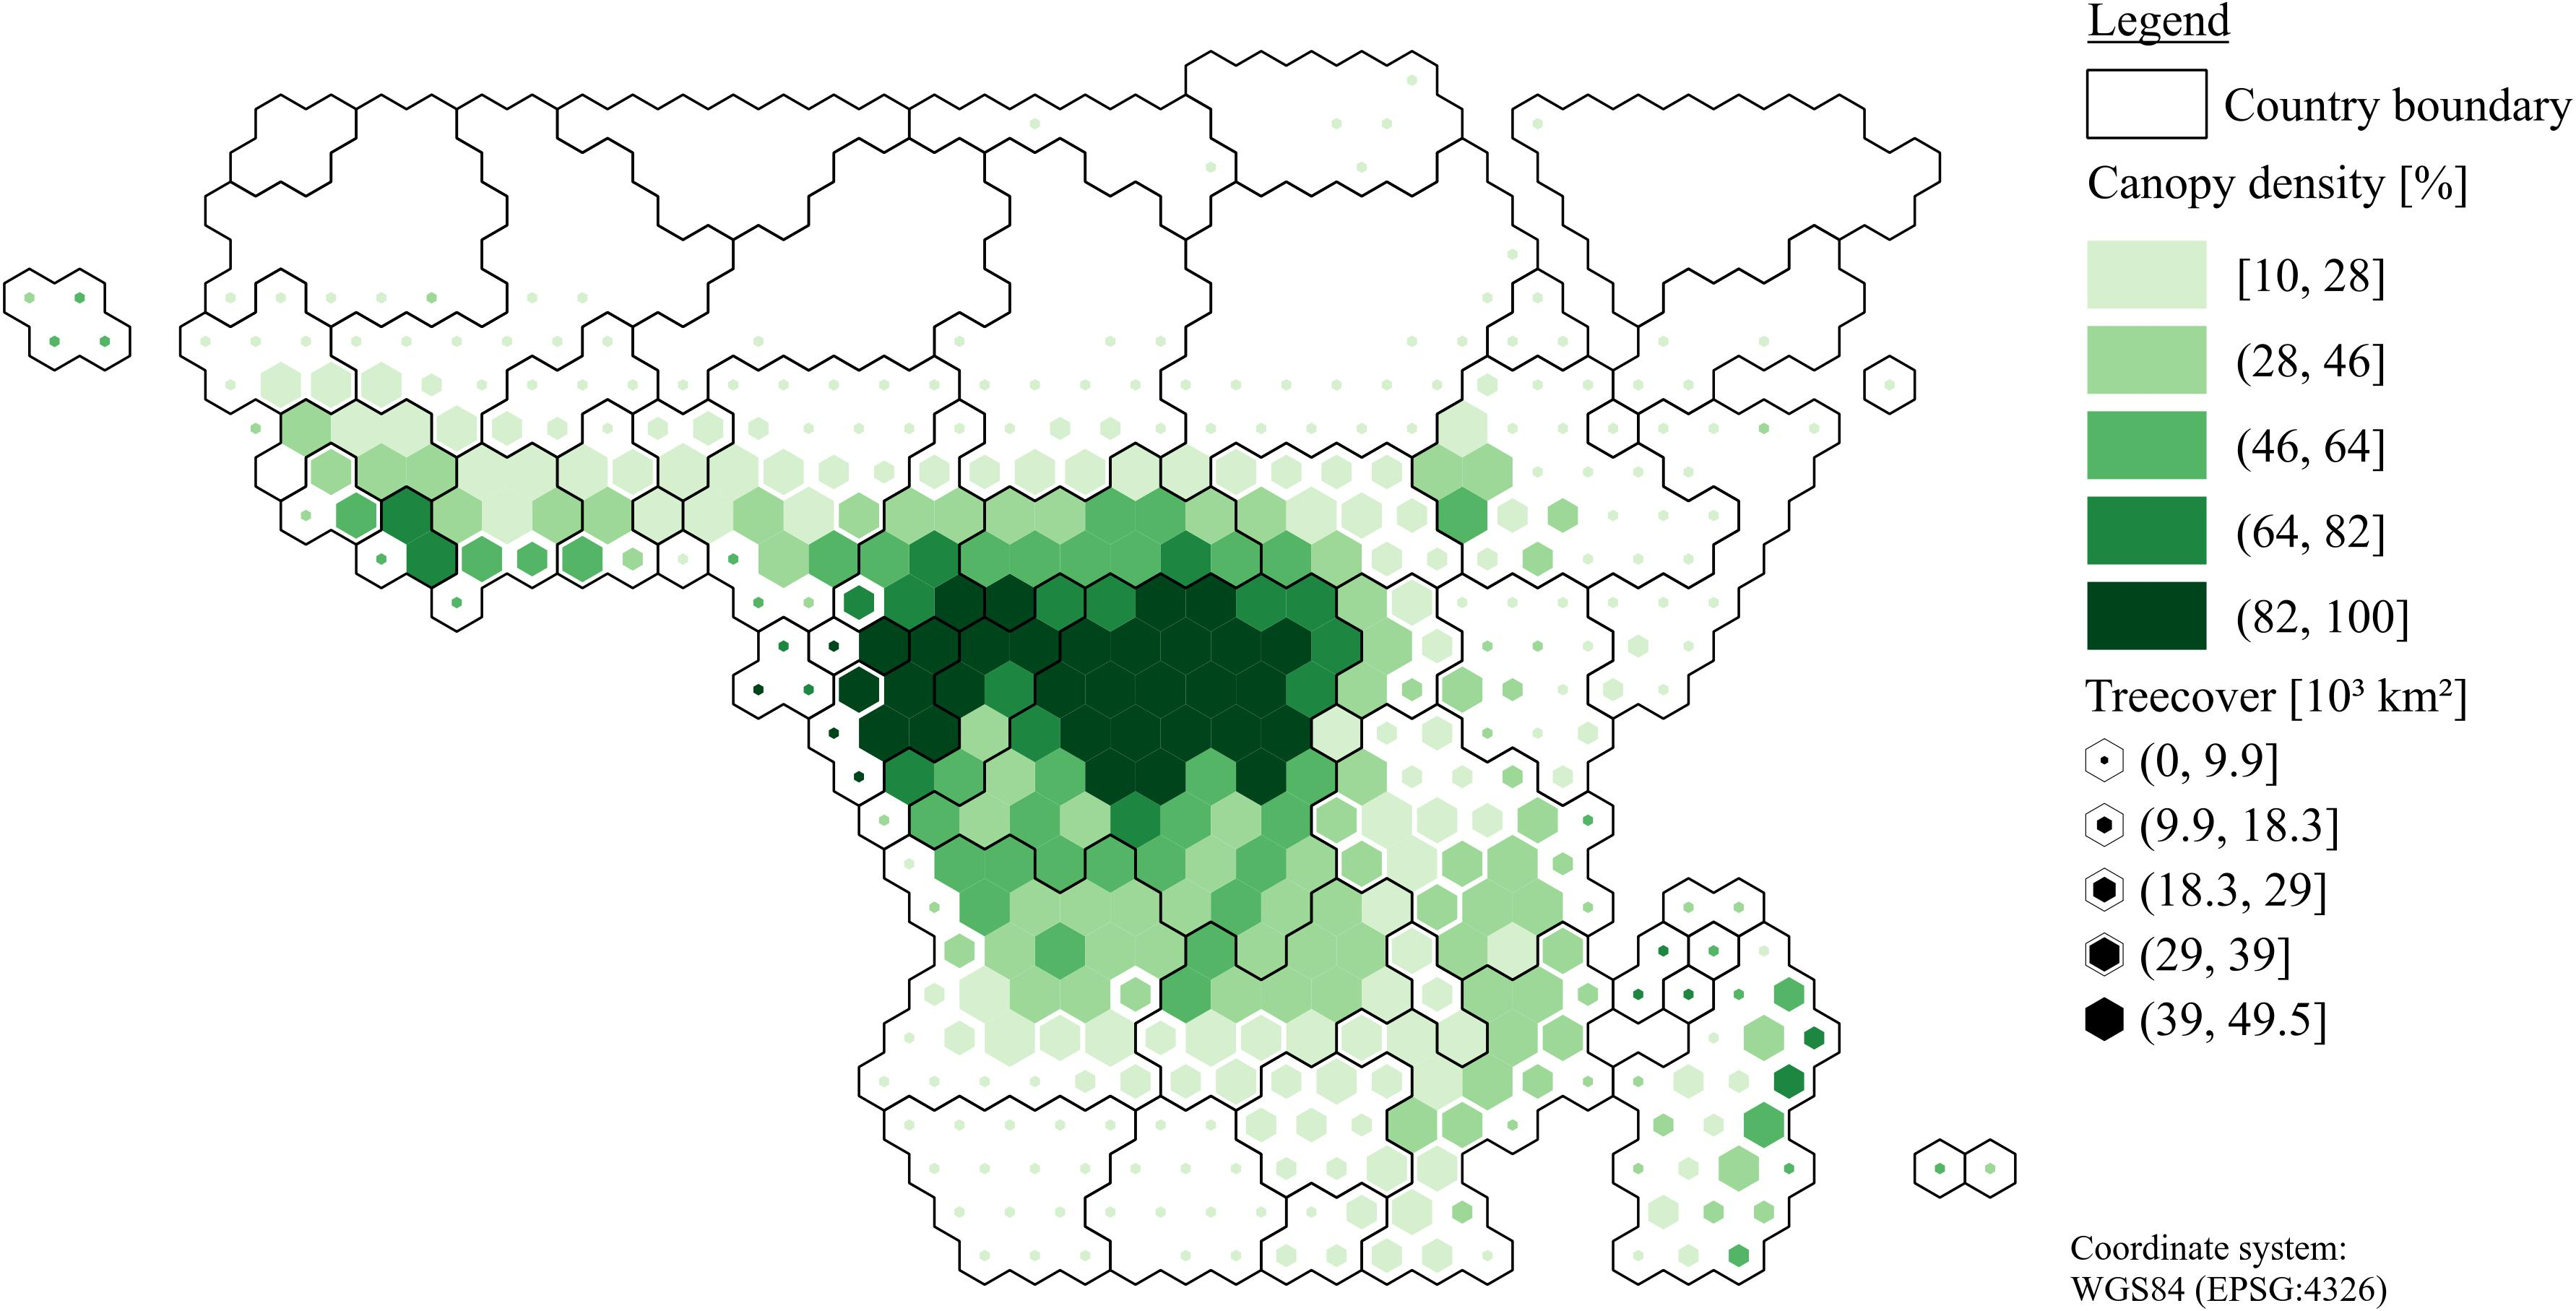
\includegraphics[scale=1]{img/africa_treecover_frameless}
%				\caption[Ecosystem service values]{}
%				\label{fig:africacover}
%			\end{figure}
%			\begin{figure}[ht]
%				\centering
%				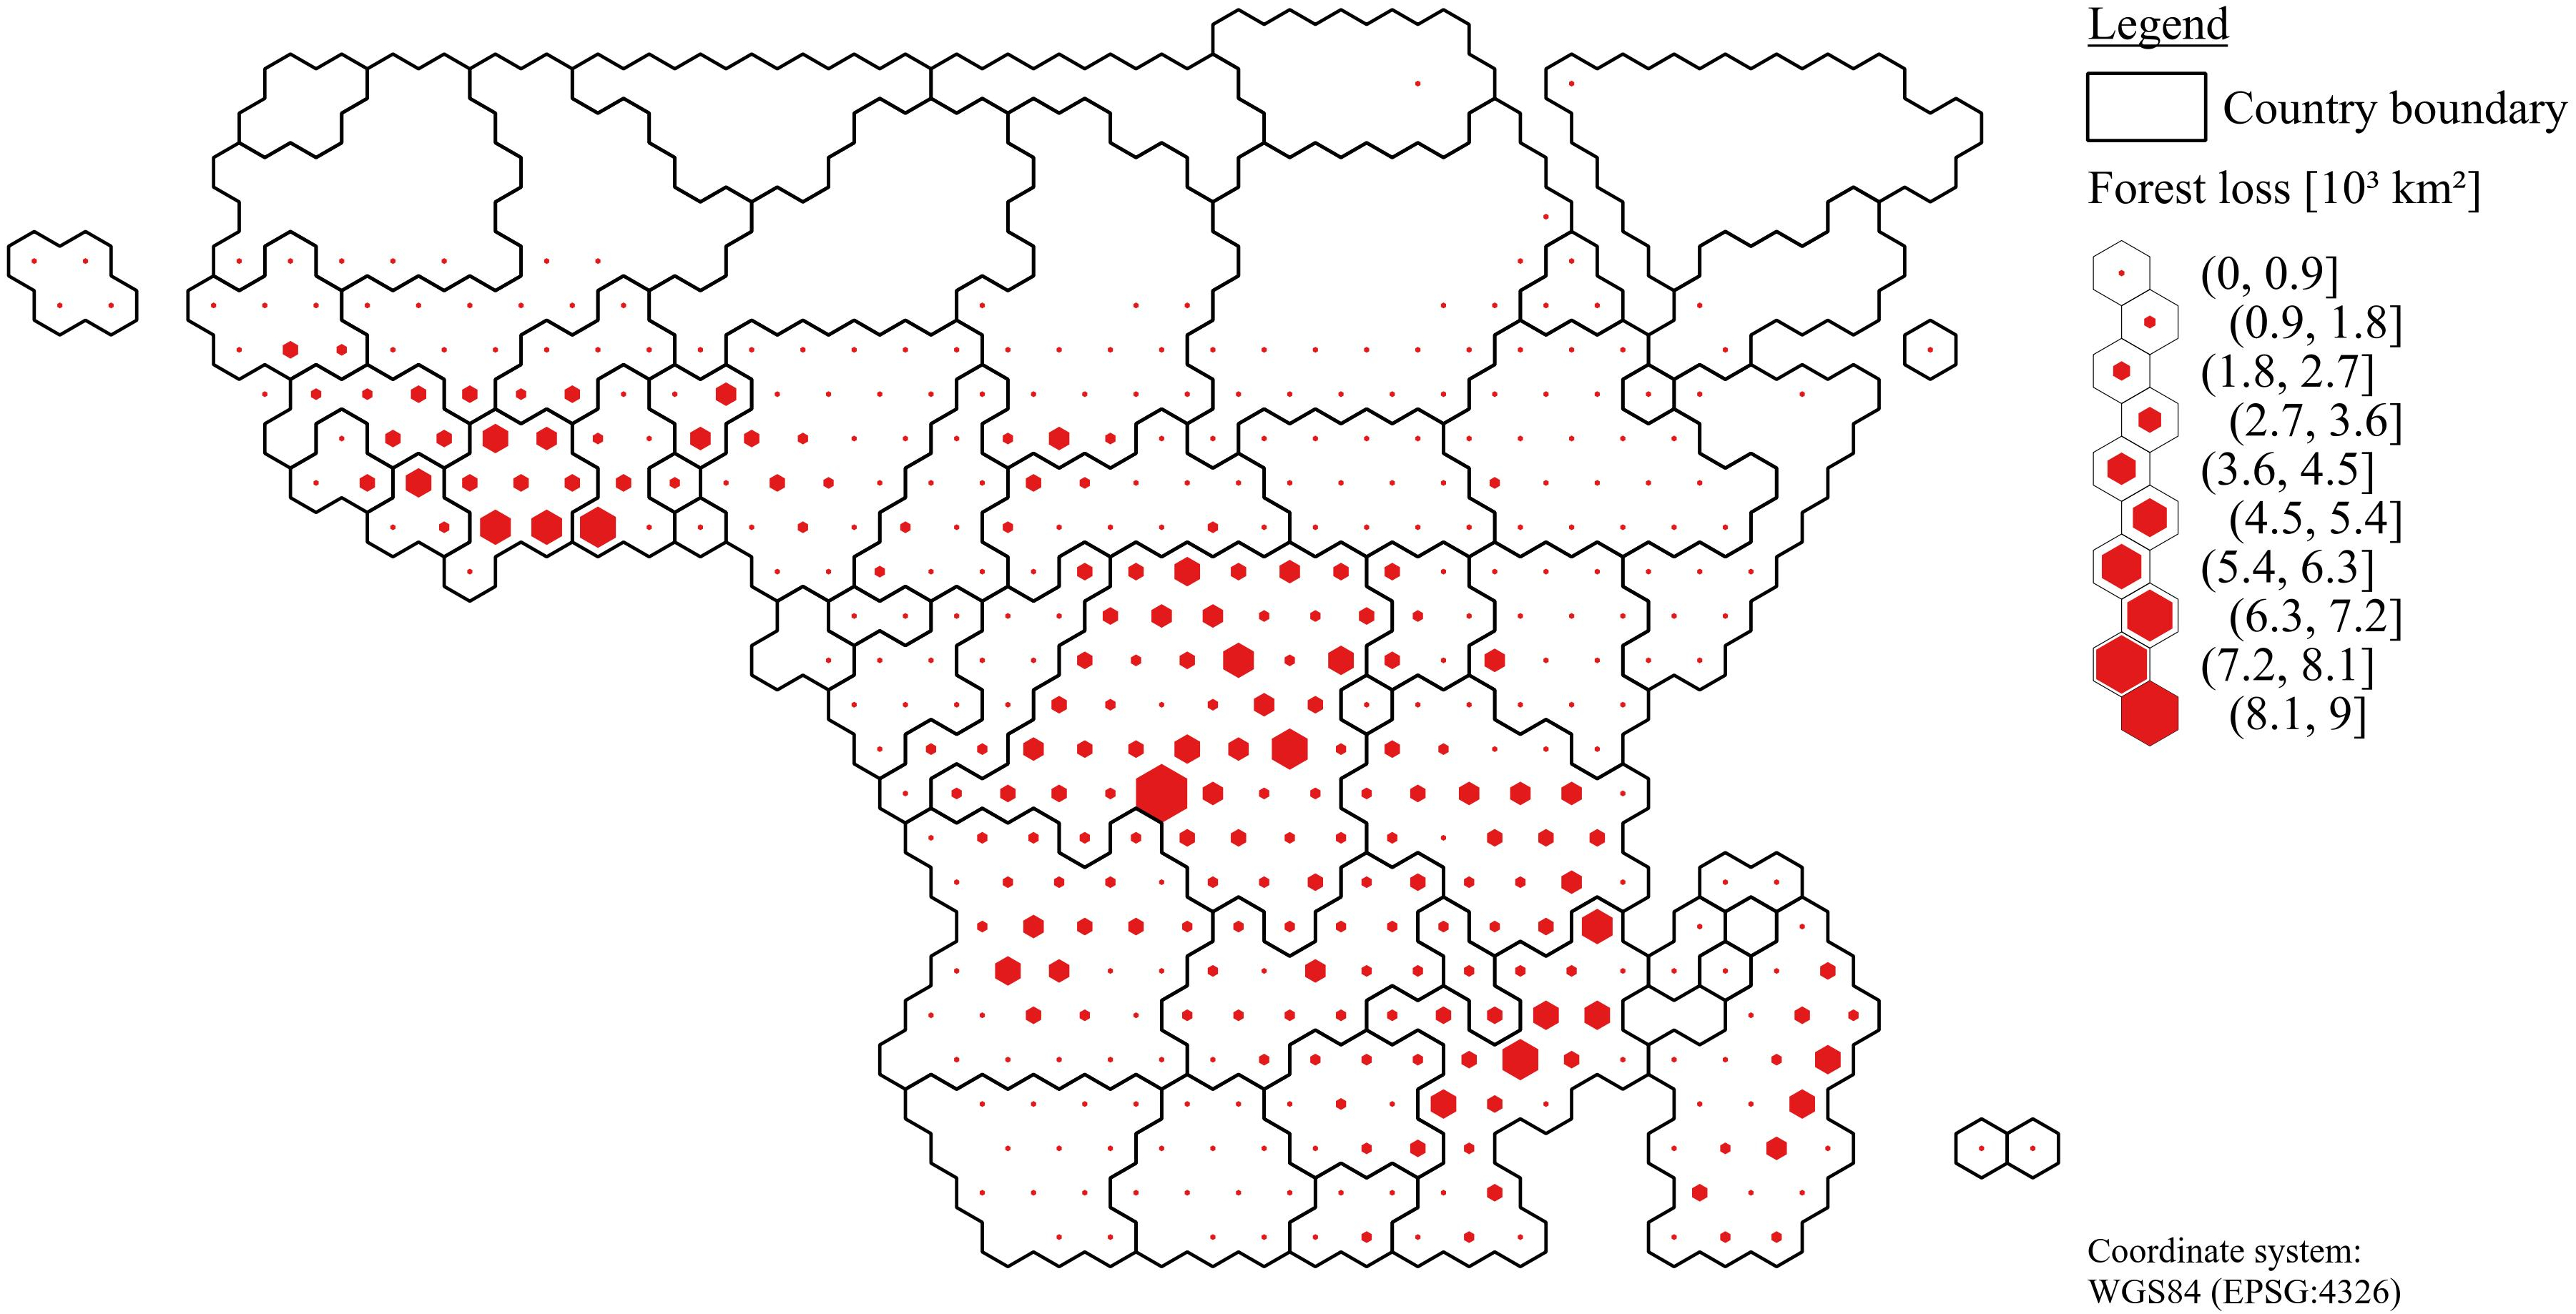
\includegraphics[scale=1]{img/africa_loss_frameless}
%				\caption[Ecosystem service values]{}
%				\label{fig:africaloss}
%			\end{figure}
%			\begin{figure}[ht]
%				\centering
%				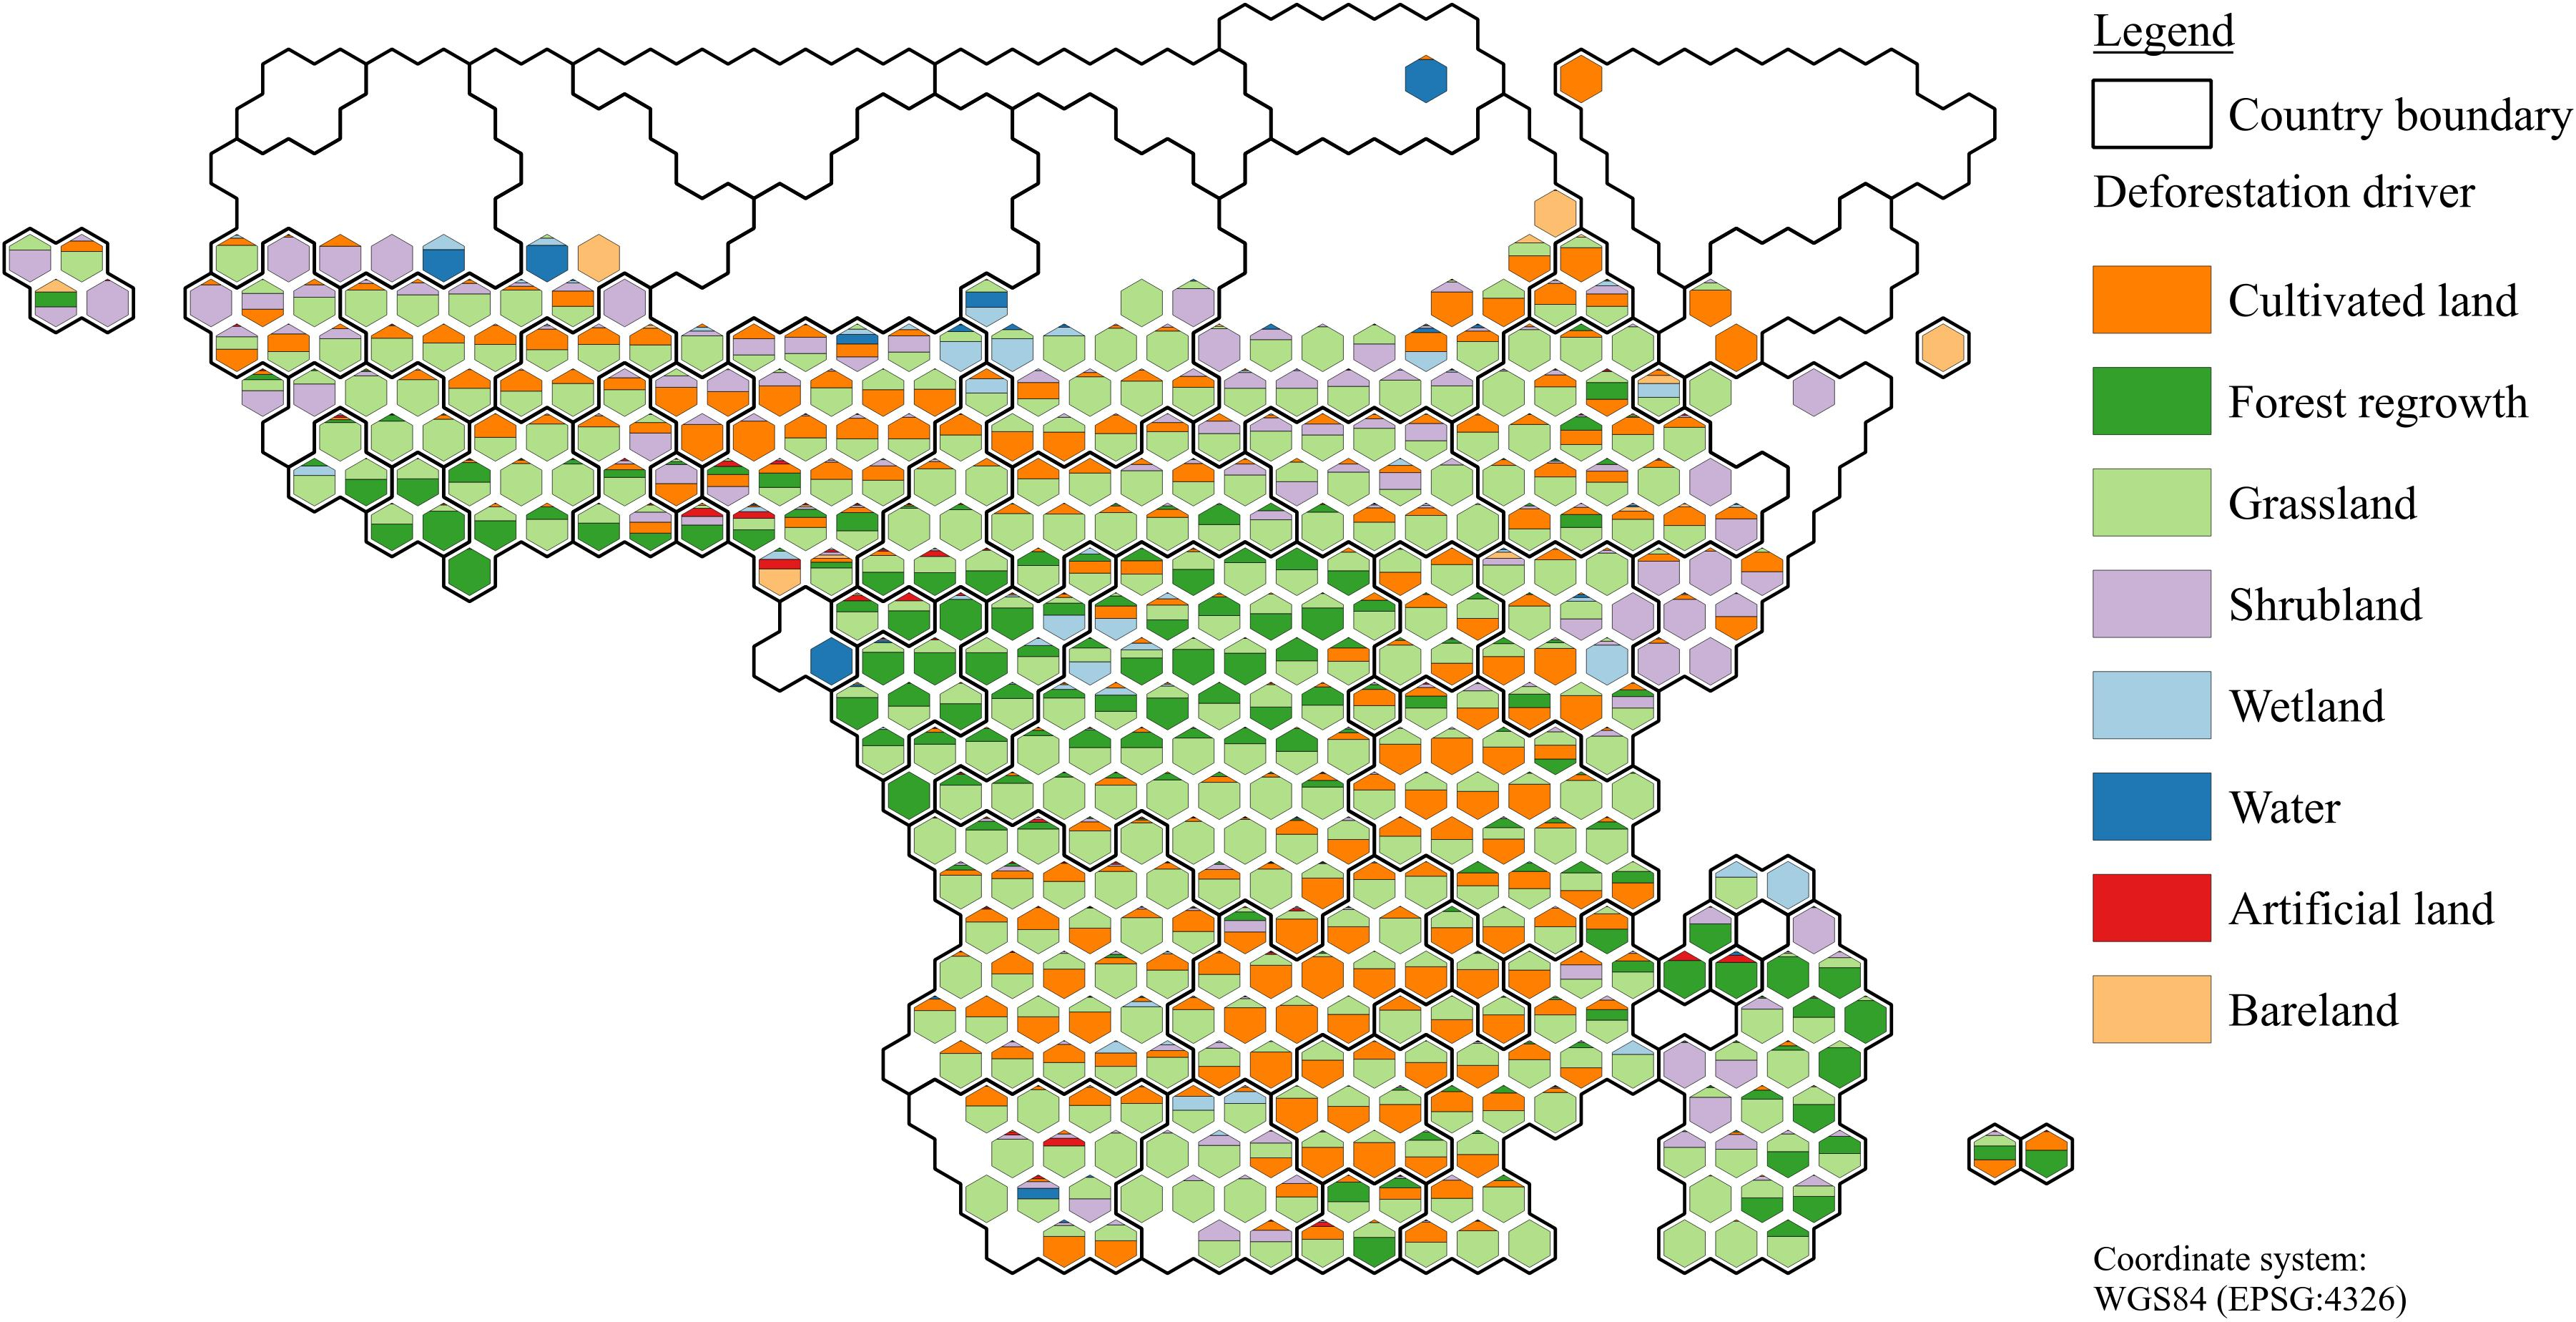
\includegraphics[scale=1]{img/africa_driver_frameless}
%				\caption[Ecosystem service values]{}
%				\label{fig:africadriver}
%			\end{figure}


% EMISSIONS
%		\begin{figure}[ht]
%			\centering
%			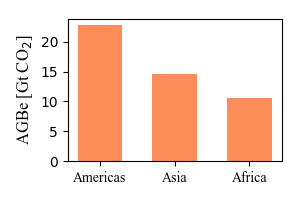
\includegraphics[scale=1]{img/agbe}
%			\caption[Ecosystem service values]{}
%			\label{fig:agbe}
%		\end{figure}
%		\begin{figure}[ht]
%			\centering
%			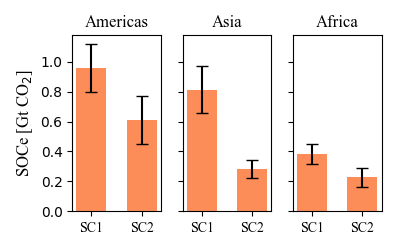
\includegraphics[scale=1]{img/soce}
%			\caption[Ecosystem service values]{}
%			\label{fig:soce}
%		\end{figure}
%
%		\begin{table}[ht]
%			\centering
%			\caption[Soil organic carbon emissions]{Soil organic carbon emissions}
%			\label{tab:soce_tab}
%			\begin{tabular}{lrrrrrrrrr}
%				\hline
%				\multirow{3}{*}{Region} & \multicolumn{3}{c}{SC1}& \multicolumn{3}{c}{SC2} & \multicolumn{3}{c}{SC3} \\
%				& \multicolumn{3}{c}{[Gt CO$_2$]}& \multicolumn{3}{c}{[Gt CO$_2$]} & \multicolumn{3}{c}{[Gt CO$_2$]} \\
%				& min & mean & max & min & mean & max & min & mean & max \\\hline
%				Americas & 0.80 & 0.96 & 1.12 & 0.45 & 0.61 & 0.77 & 0.43 & 0.59 & 0.76 \\
%				Asia & 0.66 & 0.81 & 0.97 & 0.22 & 0.28 & 0.34 & 0.22 & 0.28 & 0.33 \\
%				Africa & 0.32 & 0.39 & 0.45 & 0.17 & 0.23 & 0.29 & 0.16 & 0.23 & 0.29 \\\hline
%			\end{tabular}
%		\end{table}


% ESV
%		\begin{figure}[ht]
%			\centering
%			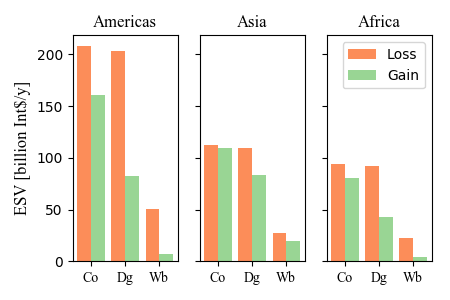
\includegraphics[scale=1]{img/esv}
%			\caption[Ecosystem service values]{}
%			\label{fig:esv}
%		\end{figure}



	\newpage
		\chapter{Discussion and Conclusion}
\label{ch:discussion}
%TODO Research question
%TODO Deforestation mechanisms
%TODO Literature - compare your work to others
%TODO Strength - selling points
%TODO Limitations
%TODO Future research opportunitie

	\section{Software, design and technology}

	\section{Deforestation}
	\label{sec:discussion_deforestation}

		\subsection{Forest definition}
		\label{subsec:discussion_forest_definition}
			\begin{itemize}
				\item For a regional approach a better solution could be to select for each region independently the right canopy density. For America a good agreement between the tree cover could be achieved by selecting the second class. For Asia by selecting the first class and for africa the second. Even better would be to decide per tile individually which canopy density should be selected. This would eliminate regional effects of different forest densities.
				\item discuss regions independently asia and america have large tree cover agreement
				\item africa has the lowest agreement only core forest zones show high similarity
				\item We can see at which regions Chen et al switched their tree cover definition to 10
				\item To improve we should apply for each tile a canopy class decision based on our analysis
				\item This could improve the improve the similarity (accuracy) by maximizing the sample count
				\item Algorithm draft for single similarity: Compute jaccard indexes for tile pair at different canopy densities, put results in a list, sort the list in decreasing order, pick the class where jaccard index is max
				\item Use this jaccard method to exclude tiles where the tree cover similarity fall below a certain threshold
			\end{itemize}

		\subsection{Tree cover and deforestation}
		\label{subsec:discussion_tree_cover_and_deforestation}

		\subsection{Proximate deforestation driver}
		\label{subsec:discussion_proxy_deforestation_driver}
			\begin{itemize}
				\item Reclassification is not a good idea cause this approach leads not to consistent results
				\item limitation the conversion of tree cover to shrubland or grassland in Africa can be mapping error
			\end{itemize}

		\subsection{Accuracy assessment}
		\label{subsec:discussion_accuracy_assessment}
			\begin{itemize}
				\item Is largely subjective because it is prepared from the study author
				\item Better if someone independent does it 
				\item Even better if you have ground truth prepared by field studies
				\item Class variability errors source the reclassification
				\item Time frame of our classification we classified our ground truth data at google image data
				\item Land cover change dynamics stay hidden
				\item Sample size is not scientific chosen
				\item Confusion matrix neglect uncertainty, apply approach in olofsson et al should improve the reasoning
				\item mention that kappa coefficient should be neglected cause issues reference olofsson 
			\end{itemize}

	\section{Emissions}

	\section{Ecosystem service values}
		\begin{itemize}
			\item resilience of esv loss could be achieved over optimizing total value of the new land-use
			\item target optimization is use the clearcut by maximizing profit and minimizing the esv loss
			\item large differences between the datasets
		\end{itemize}

	\section{Binning analysis and visualization}
		\begin{itemize}
			\item Cut polygon by line the Scala (1992) approach explained with parametric separation function, and bezier
			\item A approach where ratio is also ratio of the hexagon area
		\end{itemize}


	\newpage
%		\section*{Acknowledgements}
\label{sec:acknow}
\addcontentsline{toc}{section}{Acknowledgements}
%	\newpage


	\pagenumbering{Roman}
	\setcounter{page}{1}


		% references
		\addcontentsline{toc}{section}{References}
\bibliography{lit}
% \citet cite textual
% \citep cite parenthetical
% \citep* or \citet* full author list
% all commands accept one or two options for text before and after citation
% one option post-note, two options pre- and post-note
% \citep[foo][bar]{key}
	\newpage

		% lists
		\listoffigures

\listoftables

\chapter*{List of Abbreviations}
\addcontentsline{toc}{chapter}{List of Abbreviations}
\begin{singlespace}
	\begin{acronym}[GSOCmap]
		\setlength{\itemsep}{-\parsep}
		\acro{AGB}{Aboveground live woody Biomass density}
		\acro{AISM}{aligned image stack mosaic}
		\acro{API}{application programming interface}
		\acro{CRS}{coordinate reference system}
		\acro{ESV}{ecosystem service value}
		\acro{FAO}{Food and Agriculture Organization}
		\acro{GFC}{University of Maryland Global Forest Change}
		\acro{GFW}{Global Forest Watch}
		\acro{GHG}{greenhouse gas}
		\acro{GL30}{GlobeLand30}
		\acro{GSOCmap}{Global Soil Organic Carbon map}
		\acro{GTiff}{Geo-Tiff}
		\acro{IFL}{Intact Forest Landscapes}
		\acro{JI}{Jaccard Index}
		\acro{LC}{land cover}
		\acro{LU}{land use}
		\acro{PDD}{proximate deforestation driver}
		\acro{SHP}{Shapefile}
		\acro{SOC}{soil organic carbon}
		\acro{URL}{uniform resource locator}
		\acro{UTM}{Universal Transverse Mercator}
		\acro{WGS84}{World Geodetic System 1984}
	\end{acronym}
\end{singlespace}











	\newpage

		% appendix
		\chapter*{Appendix}
\label{chap:appendix}
\addcontentsline{toc}{chapter}{Appendix}
%TODO holm correction to both tables
%TODO add to table class codes

	\begin{table}[ht]
		\centering
		\caption[Comparison of tree cover agreement between regions]{\textbf{Comparison of tree cover agreement between regions:} This table shows, a comparison of tree cover agreement between regions. The classes $JI_0$, $JI_1$, $JI_2$, and $JI_3$ as row and column headings account for the canopy density classes (0,100], (10,100], (20,100], and (30,100], respectively. The test hypothesis is H$_0$: $X_1=X_2$ where $X_1$ is the column $JI_n$ class and $X_2$ the row $JI_n$ class. The significance is indicated by $p^{*}<0.05$, $p^{**}<0.02$, and $p^{***}<0.01$.}
		\label{tab:wilcoxononesided_comparison}
		\begin{tabular}{llllllllll}
			\hline
			& & \multicolumn{4}{|c}{Americas} & \multicolumn{4}{|c|}{Asia} \\
			& Cls & JI$_0$ & JI$_1$ & JI$_2$ & JI$_3$ & JI$_0$ & JI$_1$ & JI$_2$ & JI$_3$ \\\hline
			\multirow{4}{*}{\STAB{\rotatebox[origin=c]{90}{Asia}}}
			& JI$_0$ & .02$^*$ & - & - & - & - & - & - & - \\
			& JI$_1$ & - & .02$^*$ & - & - & - & - & - & - \\
			& JI$_2$ & - & - & .03$^*$ & - & - & - & - & - \\
			& JI$_3$ & - & - & - & .05$^*$ & - & - & - & - \\\cline{1-1}
			\multirow{4}{*}{\STAB{\rotatebox[origin=c]{90}{Africa}}} 
			& JI$_0$ & .00$^{***}$ & - & - & - & .00$^{***}$ & - & - & - \\
			& JI$_1$ & - & .00$^{***}$ & - & - & - & .00$^{***}$ & - & - \\
			& JI$_2$ & - & - & .00$^{***}$ & - & - & - & .00$^{***}$ & - \\
			& JI$_3$ & - & - & - & .00$^{***}$ & - & - & - & .00$^{***}$ \\\hline
		\end{tabular}
	\end{table}
	
	\begin{table}[ht]
		\centering
		\caption[Comparison of tree cover agreement between regions]{\textbf{Comparison of tree cover agreement between regions:} This table shows, a comparison of tree cover agreement between regions and the direction of differences. The classes $JI_0$, $JI_1$, $JI_2$, and $JI_3$ as row and column headings account for the canopy density classes (0,100], (10,100], (20,100], and (30,100], respectively. The test hypothesis is H$_0$: $X_1\leq X_2$ where $X_1$ is the column $JI_n$ class and $X_2$ the row $JI_n$ class. The significance is indicated by $p^{*}<0.05$, $p^{**}<0.025$, $p^{***}<0.01$, and $p^{\dagger}<0.005$.}
		\label{tab:wilcoxontwosided_comparison}
		\begin{tabular}{llllllllll}
			\hline
			& & \multicolumn{4}{|c}{Americas} & \multicolumn{4}{|c|}{Asia} \\
			& Cls & JI$_0$ & JI$_1$ & JI$_2$ & JI$_3$ & JI$_0$ & JI$_1$ & JI$_2$ & JI$_3$ \\\hline
			\multirow{4}{*}{\STAB{\rotatebox[origin=c]{90}{Asia}}}
			& JI$_0$ & .99 & - & - & - & - & - & - & - \\
			& JI$_1$ & - & .99 & - & - & - & - & - & - \\
			& JI$_2$ & - & - & .99 & - & - & - & - & - \\
			& JI$_3$ & - & - & - & .99 & - & - & - & - \\\cline{1-1}
			\multirow{4}{*}{\STAB{\rotatebox[origin=c]{90}{Africa}}} 
			& JI$_0$ & .00$^{\dagger}$ & - & - & - & .00$^{\dagger}$ & - & - & - \\
			& JI$_1$ & - & .00$^{\dagger}$ & - & - & - & .00$^{\dagger}$ & - & - \\
			& JI$_2$ & - & - & .00$^{\dagger}$ & - & - & - & .00$^{\dagger}$ & - \\
			& JI$_3$ & - & - & - & .00$^{\dagger}$ & - & - & - & .00$^{\dagger}$ \\\hline
		\end{tabular}
	\end{table}


	\begin{landscape}
		\begin{figure}[ht]
				\centering
				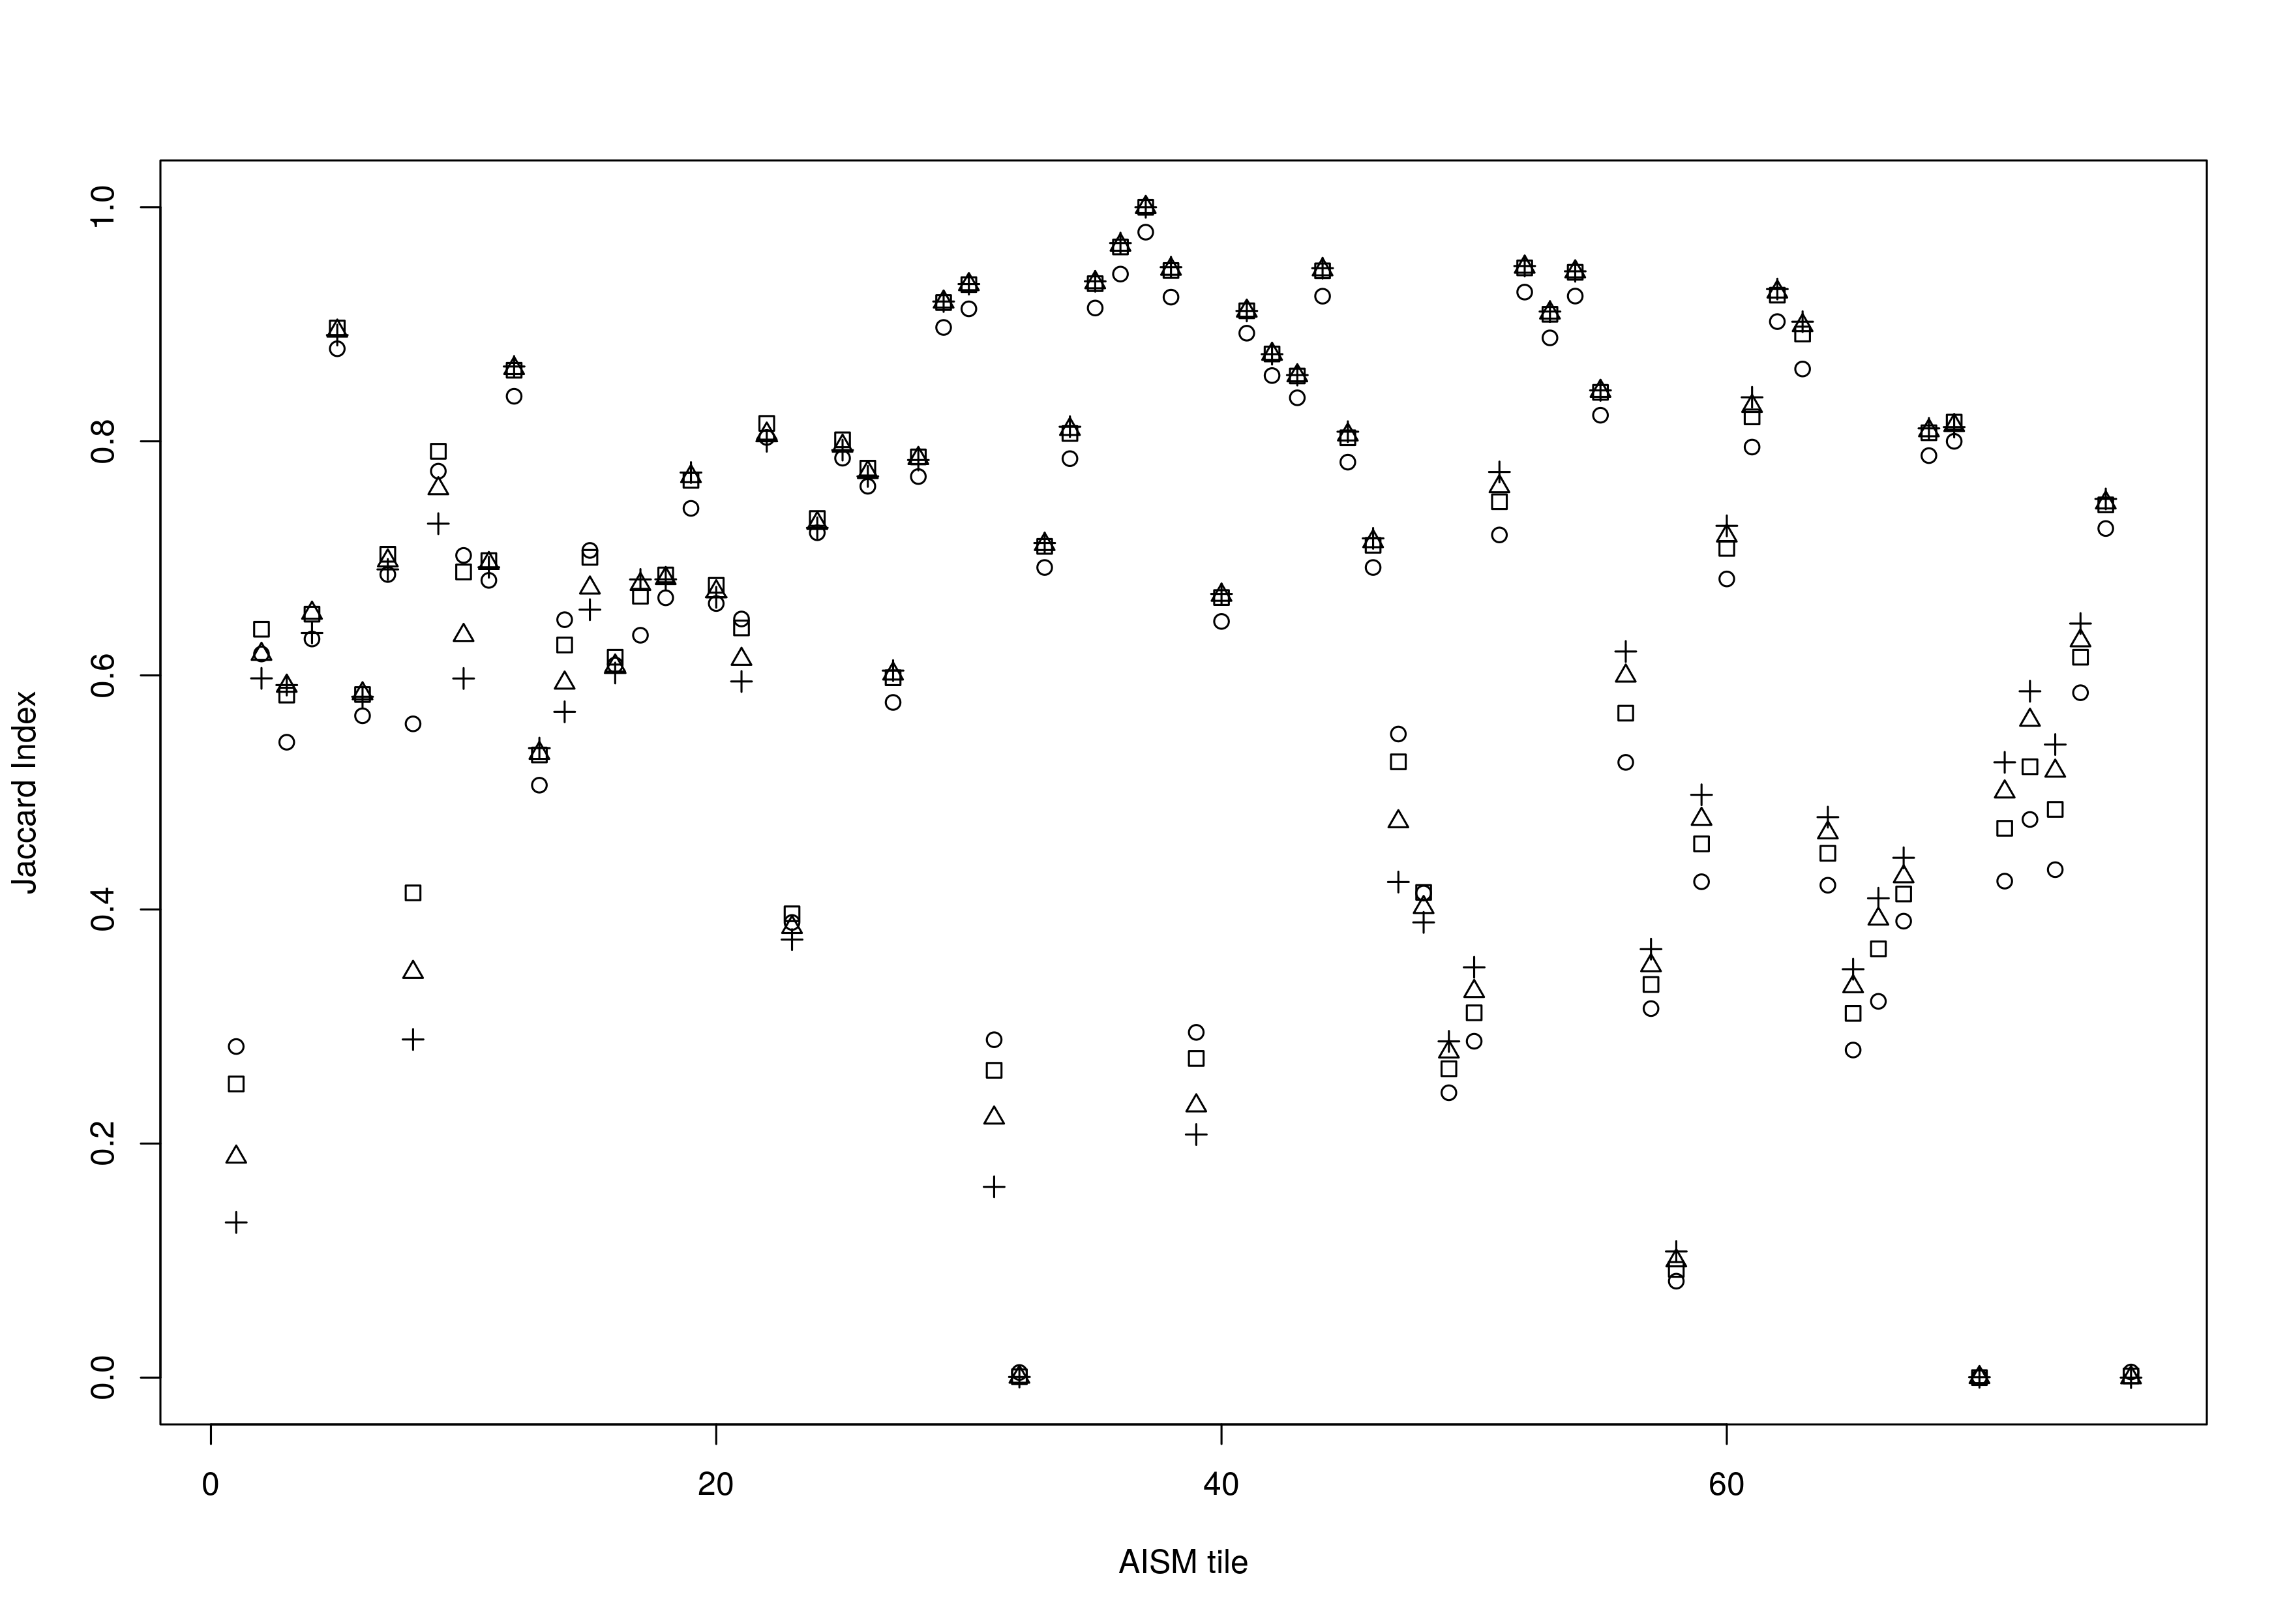
\includegraphics[scale=.65]{img/jaccard_tiles_americas}
				\caption[Caption]{\textbf{Caption:} Caption}
				\label{fig:jaccard_americas_appendix}
		\end{figure}
	\end{landscape}

	\begin{landscape}
		\begin{figure}[ht]
			\centering
			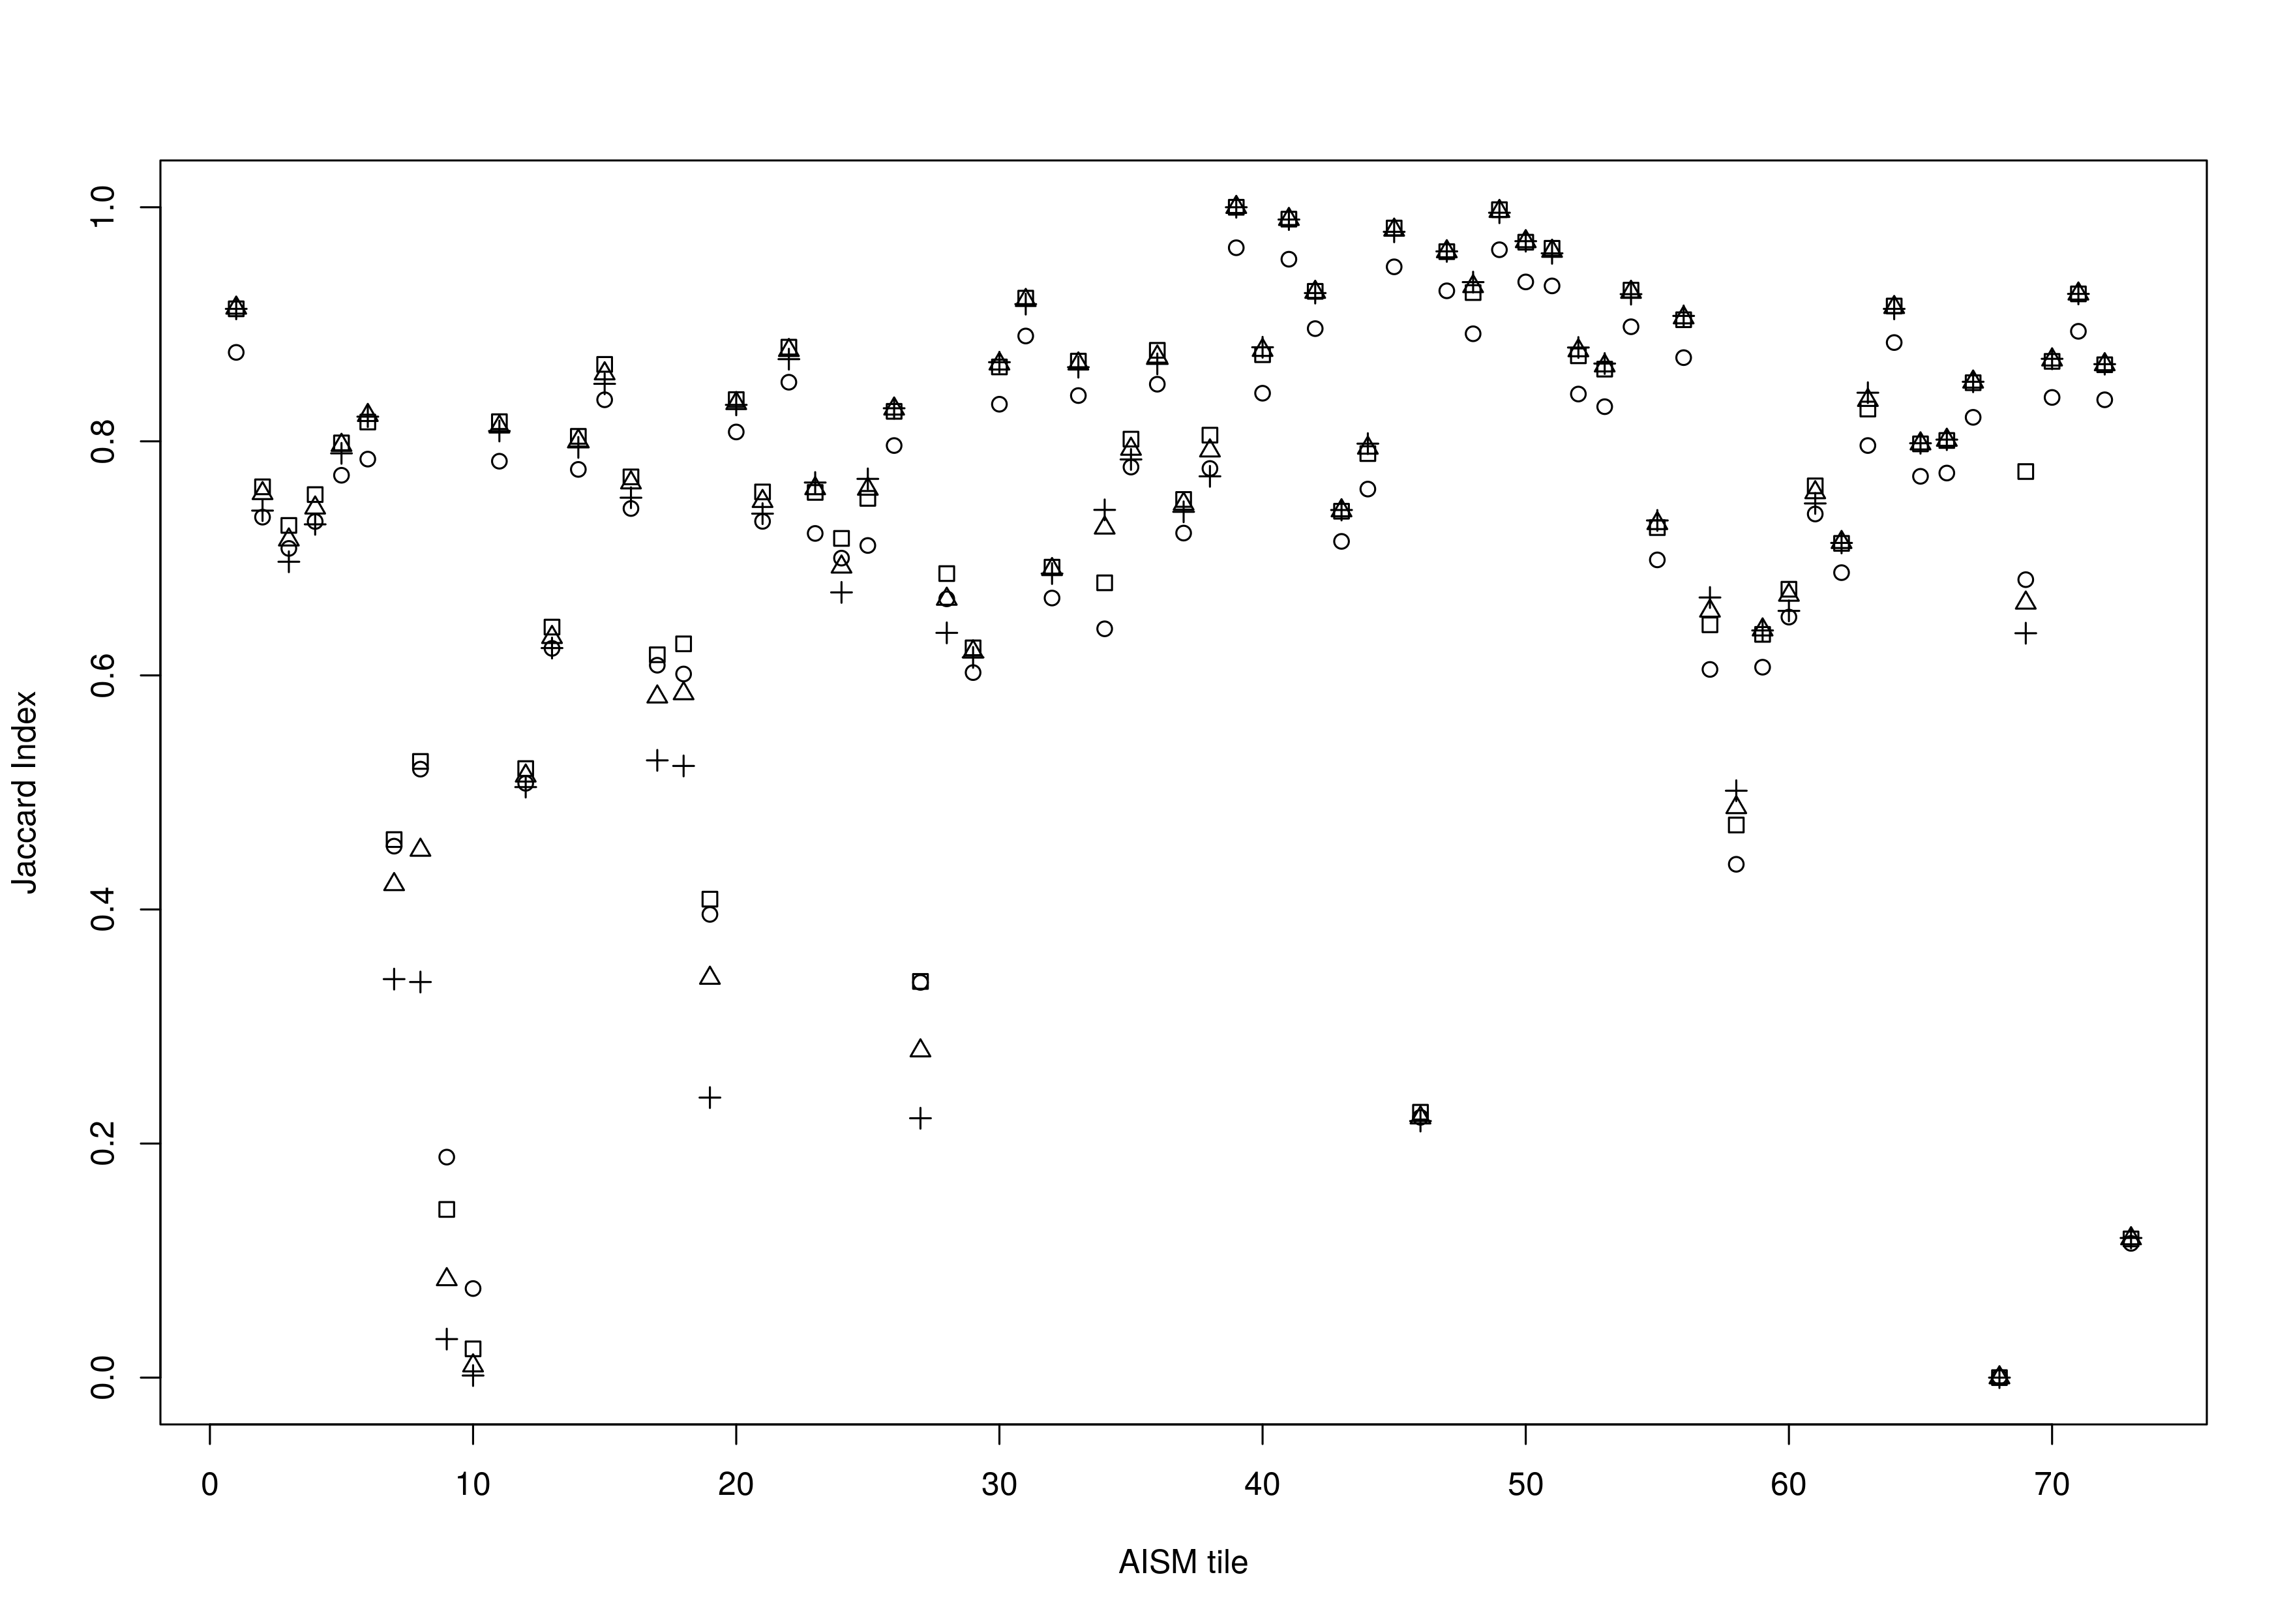
\includegraphics[scale=.65]{img/jaccard_tiles_asia}
			\caption[Caption]{\textbf{Caption:} Caption}
			\label{fig:jaccard_asia_appendix}
		\end{figure}
	\end{landscape}

	\begin{landscape}
		\begin{figure}[ht]
			\centering
			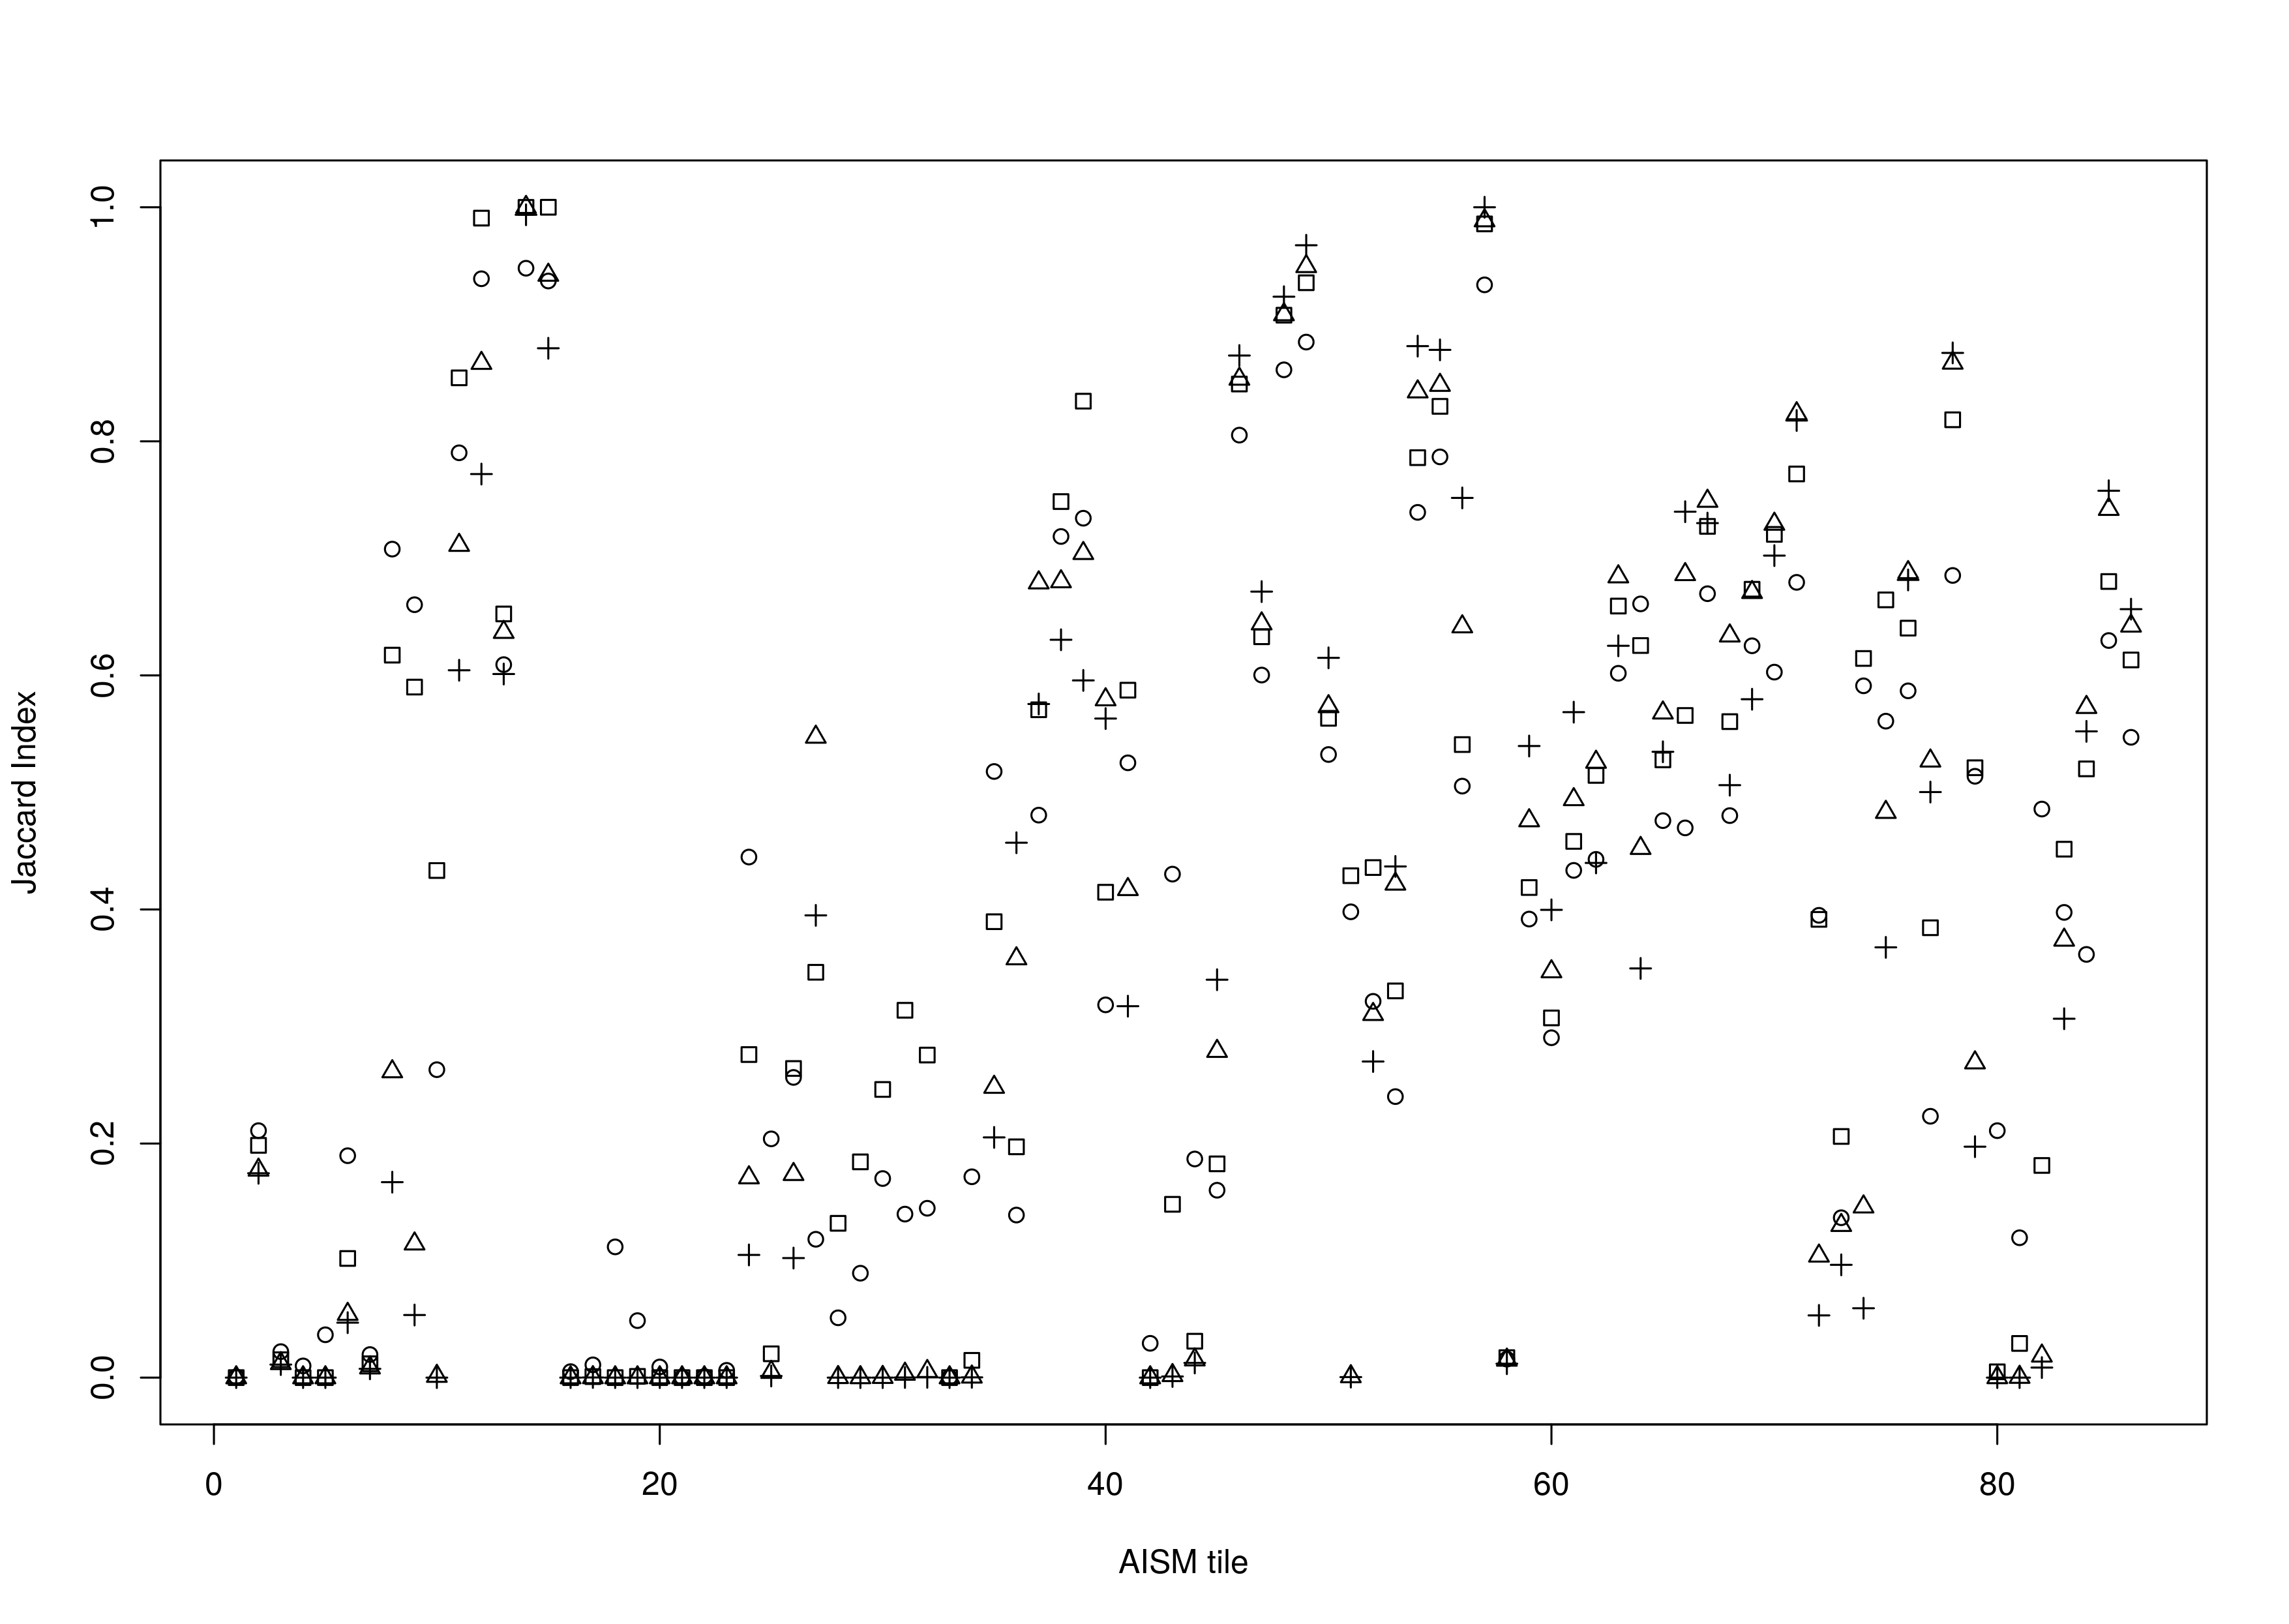
\includegraphics[scale=.65]{img/jaccard_tiles_africa}
			\caption[Caption]{\textbf{Caption:} Caption}
			\label{fig:jaccard_africa_appendix}
		\end{figure}
	\end{landscape}

	\begin{scriptsize}
	\begin{landscape}
		\begin{center}
			\begin{longtable}[ht]{lrrrrrrrrrr}
			\caption[Estimates of proximate drivers of deforestation for countries, continents, and tropical zone]{\textbf{Estimates of proximate drivers of deforestation for countries, continents, and tropical zone:}} \label{tab:proximate_driver}\\

			\hline
			Region&Cultivated&Forest&Regrowth&Grassland&Shrubland&Water&Artificial&Bareland&Total&Total$^\dagger$\\
			\hline
			\endfirsthead

			%\caption[]{continued}\\
			\hline
			Region&Cultivated&Forest&Regrowth&Grassland&Shrubland&Water&Artificial&Bareland&Total&Total$^\dagger$\\
			\hline
			\endhead

			\hline
			\endfoot

			%South America
			Argentina&5733.9 (65.8\%)&1380.6 (15.9\%)&147.9 (1.7\%)&461.8 (5.3\%)&718.7 (8.3\%)&230.8 (2.7\%)&32.8 (0.4\%)&2.0 (0.0\%)&8708.5&7097.1\\
			Bahamas&0.0 (0.0\%)&3.3 (41.2\%)&0.1 (1.3\%)&0.0 (0.0\%)&0.3 (3.8\%)&3.0 (37.5\%)&1.3 (16.3\%)&0.0 (0.0\%)&8.0&1.7\\
			Belize&212.2 (24.4\%)&113.0 (13.0\%)&155.5 (17.9\%)&308.9 (35.6\%)&54.5 (6.3\%)&12.7 (1.5\%)&11.1 (1.3\%)&0.0 (0.0\%)&867.9&742.2\\
			Bolivia&9288.2 (37.2\%)&5106.4 (20.5\%)&2428.1 (9.7\%)&5581.0 (22.4\%)&1825.1 (7.3\%)&590.8 (2.4\%)&108.3 (0.4\%)&19.5 (0.1\%)&24947.4&19250.2\\
			Brazil$^*$&56443.7 (19.1\%)&16433.7 (5.6\%)&34746.7 (11.8\%)&146802.9 (49.7\%)&35954.2 (12.2\%)&3832.4 (1.3\%)&738.8 (0.3\%)&209.0 (0.1\%)&295161.4&274895.3\\
			Chile$^*$&-&-&-&-&-&-&-&-&-&-\\
			Colombia&1297.9 (6.2\%)&5272.3 (25.2\%)&5177.2 (24.7\%)&6995.9 (33.4\%)&1593.1 (7.6\%)&573.6 (2.7\%)&26.0 (0.1\%)&9.7 (0.0\%)&20945.7&15099.8\\
			Costa Rica&307.4 (21.2\%)&536.8 (37.1\%)&178.5 (12.3\%)&397.4 (27.5\%)&11.0 (0.8\%)&7.0 (0.5\%)&9.0 (0.6\%)&0.1 (0.0\%)&1447.2&903.4\\
			Cuba&233.5 (17.6\%)&499.9 (37.7\%)&181.2 (13.7\%)&330.4 (24.9\%)&23.2 (1.8\%)&35.2 (2.7\%)&6.2 (0.5\%)&15.7 (1.2\%)&1325.3&790.2\\
			Dominican Republic&81.6 (5.4\%)&763.5 (50.5\%)&122.2 (8.1\%)&510.8 (33.8\%)&2.9 (0.2\%)&4.2 (0.3\%)&13.3 (0.9\%)&13.1 (0.9\%)&1511.6&743.9\\
			Ecuador&1143.9 (28.2\%)&1163.7 (28.7\%)&823.3 (20.3\%)&735.7 (18.1\%)&142.2 (3.5\%)&34.7 (0.9\%)&8.0 (0.2\%)&6.3 (0.2\%)&4057.8&2859.4\\
			El Salvador&58.1 (11.6\%)&28.2 (5.7\%)&6.2 (1.2\%)&390.9 (78.3\%)&8.5 (1.7\%)&1.6 (0.3\%)&5.6 (1.1\%)&0.0 (0.0\%)&499.1&469.3\\
			French Guiana&46.9 (14.7\%)&52.8 (16.5\%)&100.0 (31.2\%)&91.4 (28.6\%)&0.0 (0.0\%)&7.8 (2.4\%)&20.6 (6.4\%)&0.5 (0.2\%)&320.0&259.4\\
			Guatemala&1843.2 (23.9\%)&1172.6 (15.2\%)&924.2 (12.0\%)&2974.9 (38.6\%)&733.1 (9.5\%)&21.2 (0.3\%)&39.6 (0.5\%)&0.0 (0.0\%)&7708.8&6515.0\\
			Guyana&22.1 (3.1\%)&244.7 (34.3\%)&274.7 (38.5\%)&134.0 (18.8\%)&10.1 (1.4\%)&19.9 (2.8\%)&8.3 (1.2\%)&0.0 (0.0\%)&713.8&449.2\\
			Haiti&8.3 (3.9\%)&146.5 (69.3\%)&13.9 (6.6\%)&40.9 (19.3\%)&0.1 (0.0\%)&0.9 (0.4\%)&0.2 (0.1\%)&0.6 (0.3\%)&211.4&64.0\\
			Honduras&101.2 (2.5\%)&1200.1 (30.0\%)&487.9 (12.2\%)&2050.5 (51.2\%)&137.8 (3.4\%)&20.4 (0.5\%)&8.9 (0.2\%)&0.0 (0.0\%)&4006.8&2786.3\\
			Jamaica&7.2 (2.8\%)&127.7 (48.8\%)&25.5 (9.7\%)&82.4 (31.5\%)&0.0 (0.0\%)&1.9 (0.7\%)&16.7 (6.4\%)&0.3 (0.1\%)&261.7&132.1\\
			Mexico$^*$&3267.8 (18.7\%)&4857.8 (27.8\%)&3763.8 (21.5\%)&3950.6 (22.6\%)&1169.5 (6.7\%)&88.8 (0.5\%)&373.4 (2.1\%)&11.1 (0.1\%)&17482.8&12536.2\\
			Nicaragua&68.9 (0.9\%)&3405.0 (45.9\%)&1567.8 (21.2\%)&2268.8 (30.6\%)&78.3 (1.1\%)&19.9 (0.3\%)&2.5 (0.0\%)&0.0 (0.0\%)&7411.2&3986.3\\
			Panama&142.2 (6.3\%)&619.7 (27.6\%)&352.8 (15.7\%)&1019.7 (45.5\%)&70.8 (3.2\%)&22.3 (1.0\%)&13.5 (0.6\%)&0.4 (0.0\%)&2241.4&1599.4\\
			Paraguay$^*$&13718.0 (48.9\%)&6383.0 (22.8\%)&216.2 (0.8\%)&2480.2 (8.8\%)&5107.2 (18.2\%)&118.8 (0.4\%)&24.9 (0.1\%)&1.2 (0.0\%)&28049.5&21547.7\\
			Peru&780.4 (6.6\%)&2333.9 (19.8\%)&3394.0 (28.8\%)&2710.8 (23.0\%)&1230.9 (10.4\%)&1213.5 (10.3\%)&27.8 (0.2\%)&102.2 (0.9\%)&11793.5&8246.1\\
			Puerto Rico&4.1 (3.7\%)&56.4 (50.5\%)&10.2 (9.1\%)&30.7 (27.5\%)&0.0 (0.0\%)&0.4 (0.4\%)&8.8 (7.9\%)&1.0 (0.9\%)&111.6&54.8\\
			Suriname&36.7 (7.4\%)&132.2 (26.8\%)&167.5 (33.9\%)&108.5 (22.0\%)&0.0 (0.0\%)&40.8 (8.3\%)&8.2 (1.7\%)&0.0 (0.0\%)&493.9&320.9\\
			Venezuela&1082.3 (10.2\%)&2758.9 (26.1\%)&1644.0 (15.5\%)&3382.4 (32.0\%)&1388.8 (13.1\%)&267.4 (2.5\%)&47.7 (0.5\%)&12.7 (0.1\%)&10584.2&7557.9\\\hline
			South America&95929.7 (21.3\%)&54792.7 (12.2\%)&56909.4 (12.6\%)&183841.5 (40.8\%)&50260.3 (11.1\%)&7170.0 (1.6\%)&1561.5 (0.3\%)&405.4 (0.1\%)&450870.5&388907.8\\\hline

			%Africa
			Algeria$^*$&-&-&-&-&-&-&-&-&-&-\\
			Angola&4818.6 (32.7\%)&697.8 (4.7\%)&452.5 (3.1\%)&8065.9 (54.7\%)&371.2 (2.5\%)&90.9 (0.6\%)&226.5 (1.5\%)&10.9 (0.1\%)&14734.3&13945.6\\
			Benin&1518.7 (58.2\%)&200.6 (7.7\%)&45.1 (1.7\%)&74.6 (2.9\%)&762.5 (29.2\%)&0.5 (0.0\%)&5.6 (0.2\%)&0.0 (0.0\%)&2607.6&2406.5\\
			Botswana$^*$&9.4 (17.9\%)&2.1 (4.0\%)&0.0 (0.0\%)&26.4 (50.2\%)&3.6 (6.8\%)&9.9 (18.8\%)&1.2 (2.3\%)&0.0 (0.0\%)&52.6&40.6\\
			Burkina Faso&510.9 (29.4\%)&4.6 (0.3\%)&0.0 (0.0\%)&1190.0 (68.5\%)&31.7 (1.8\%)&0.3 (0.0\%)&0.1 (0.0\%)&0.7 (0.0\%)&1738.3&1733.4\\
			Burundi&49.7 (30.6\%)&6.3 (3.9\%)&3.6 (2.2\%)&98.8 (60.9\%)&2.0 (1.2\%)&0.5 (0.3\%)&1.3 (0.8\%)&0.0 (0.0\%)&162.2&155.4\\
			Cameroon&337.8 (8.5\%)&938.2 (23.6\%)&717.2 (18.1\%)&1838.8 (46.3\%)&14.4 (0.4\%)&34.6 (0.9\%)&68.6 (1.7\%)&21.6 (0.5\%)&3971.2&2998.4\\
			C. African Rep.&707.3 (18.3\%)&217.1 (5.6\%)&328.4 (8.5\%)&2470.2 (64.1\%)&118.6 (3.1\%)&3.3 (0.1\%)&9.8 (0.3\%)&0.6 (0.0\%)&3855.3&3634.9\\
			Chad&1454.7 (54.7\%)&1.8 (0.1\%)&0.1 (0.0\%)&1037.5 (39.0\%)&142.2 (5.4\%)&15.9 (0.6\%)&3.1 (0.1\%)&2.4 (0.1\%)&2657.7&2640.0\\
			Congo&107.8 (4.9\%)&406.0 (18.4\%)&591.8 (26.8\%)&968.0 (43.8\%)&0.3 (0.0\%)&109.7 (5.0\%)&25.8 (1.2\%)&0.1 (0.0\%)&2209.5&1693.8\\
			DR Congo&4771.8 (9.4\%)&3518.2 (6.9\%)&13508.7 (26.6\%)&26400.4 (52.0\%)&508.2 (1.0\%)&1736.9 (3.4\%)&314.7 (0.6\%)&0.1 (0.0\%)&50759.0&45503.9\\
			Djibouti&-&-&-&-&-&-&-&-&-&-\\
			Egypt$^*$&-&-&-&-&-&-&-&-&-&-\\
			Equatorial Guinea&0.0 (0.0\%)&77.2 (28.7\%)&77.7 (28.9\%)&72.6 (27.0\%)&1.3 (0.5\%)&1.3 (0.5\%)&38.5 (14.3\%)&0.0 (0.0\%)&268.6&190.1\\
			Eritrea&0.0 (0.0\%)&0.0 (0.0\%)&0.0 (0.0\%)&0.1 (100.0\%)&0.0 (0.0\%)&0.0 (0.0\%)&0.0 (0.0\%)&0.0 (0.0\%)&0.1&0.1\\
			Ethiopia&356.8 (16.1\%)&296.9 (13.4\%)&137.2 (6.2\%)&1321.6 (59.5\%)&92.3 (4.2\%)&4.5 (0.2\%)&3.9 (0.2\%)&6.6 (0.3\%)&2219.8&1918.4\\
			Gabon&1.4 (0.1\%)&528.7 (32.9\%)&664.1 (41.3\%)&362.7 (22.5\%)&0.0 (0.0\%)&22.9 (1.4\%)&24.9 (1.5\%)&3.9 (0.2\%)&1608.6&1057.0\\
			Gambia&35.6 (29.1\%)&0.0 (0.0\%)&0.0 (0.0\%)&63.5 (51.9\%)&19.8 (16.2\%)&0.1 (0.1\%)&3.4 (2.8\%)&0.0 (0.0\%)&122.4&122.3\\
			Ghana&319.1 (6.8\%)&525.3 (11.1\%)&1523.7 (32.3\%)&1990.8 (42.2\%)&235.5 (5.0\%)&27.6 (0.6\%)&95.0 (2.0\%)&0.0 (0.0\%)&4717.0&4164.1\\
			Guinea&261.3 (8.2\%)&61.2 (1.9\%)&118.0 (3.7\%)&2296.7 (72.4\%)&419.2 (13.2\%)&3.3 (0.1\%)&11.4 (0.4\%)&2.1 (0.1\%)&3173.2&3108.7\\
			Guinea Bissau&136.7 (24.5\%)&2.3 (0.4\%)&15.5 (2.8\%)&181.5 (32.5\%)&216.6 (38.8\%)&1.2 (0.2\%)&3.9 (0.7\%)&0.0 (0.0\%)&557.7&554.2\\
			Ivory Coast&1636.4 (12.5\%)&2619.8 (20.0\%)&2515.1 (19.2\%)&6147.4 (46.9\%)&81.7 (0.6\%)&34.0 (0.3\%)&69.1 (0.5\%)&0.7 (0.0\%)&13104.2&10450.4\\
			Kenya&1178.9 (48.1\%)&118.8 (4.9\%)&213.6 (8.7\%)&832.7 (34.0\%)&85.7 (3.5\%)&13.7 (0.6\%)&4.2 (0.2\%)&1.6 (0.1\%)&2449.2&2316.7\\
			Liberia&8.1 (0.2\%)&395.4 (12.0\%)&1863.5 (56.6\%)&986.7 (30.0\%)&3.5 (0.1\%)&2.2 (0.1\%)&30.7 (0.9\%)&0.0 (0.0\%)&3290.1&2892.5\\
			Libya$^*$&-&-&-&-&-&-&-&-&-&-\\
			Madagascar&197.1 (1.6\%)&667.1 (5.3\%)&5126.0 (40.6\%)&5627.5 (44.6\%)&957.9 (7.6\%)&43.5 (0.3\%)&1.5 (0.0\%)&0.1 (0.0\%)&12620.7&11910.1\\
			Malawi&457.8 (40.0\%)&185.4 (16.2\%)&83.6 (7.3\%)&398.3 (34.8\%)&8.3 (0.7\%)&1.9 (0.2\%)&4.6 (0.4\%)&4.7 (0.4\%)&1144.6&957.3\\
			Mali&480.6 (39.4\%)&1.0 (0.1\%)&0.0 (0.0\%)&708.7 (58.1\%)&25.6 (2.1\%)&0.6 (0.0\%)&2.9 (0.2\%)&0.3 (0.0\%)&1219.7&1218.1\\
			Mauritania&0.0 (0.0\%)&0.0 (0.0\%)&0.0 (0.0\%)&0.2 (33.3\%)&0.4 (66.7\%)&0.0 (0.0\%)&0.0 (0.0\%)&0.0 (0.0\%)&0.6&0.6\\
			Morocco$^*$&-&-&-&-&-&-&-&-&-&-\\
			Mozambique$^*$&6419.1 (32.7\%)&1527.7 (7.8\%)&1967.4 (10.0\%)&8959.4 (45.6\%)&664.8 (3.4\%)&49.2 (0.3\%)&37.0 (0.2\%)&17.8 (0.1\%)&19642.4&18065.5\\
			Namibia$^*$&46.1 (38.0\%)&6.8 (5.6\%)&0.0 (0.0\%)&59.9 (49.4\%)&5.1 (4.2\%)&2.1 (1.7\%)&1.0 (0.8\%)&0.2 (0.2\%)&121.2&112.3\\
			Niger&0.0 (0.0\%)&0.0 (0.0\%)&0.0 (0.0\%)&0.9 (10.3\%)&0.0 (0.0\%)&7.8 (89.7\%)&0.0 (0.0\%)&0.0 (0.0\%)&8.7&0.9\\
			Nigeria&2392.5 (34.4\%)&1462.3 (21.0\%)&452.3 (6.5\%)&1754.3 (25.2\%)&689.8 (9.9\%)&24.4 (0.4\%)&122.3 (1.8\%)&63.6 (0.9\%)&6961.5&5474.8\\
			Rwanda&65.9 (42.7\%)&18.2 (11.8\%)&16.3 (10.6\%)&46.3 (30.0\%)&5.8 (3.8\%)&0.6 (0.4\%)&1.2 (0.8\%)&0.0 (0.0\%)&154.3&135.5\\
			Senegal&221.4 (30.0\%)&0.3 (0.0\%)&0.1 (0.0\%)&401.5 (54.4\%)&112.2 (15.2\%)&0.7 (0.1\%)&1.6 (0.2\%)&0.0 (0.0\%)&737.8&736.8\\
			Sierra Leone&11.1 (0.7\%)&167.3 (10.1\%)&455.9 (27.5\%)&995.0 (60.1\%)&6.1 (0.4\%)&3.2 (0.2\%)&16.3 (1.0\%)&0.0 (0.0\%)&1654.9&1484.4\\
			Somalia&7.2 (11.0\%)&10.0 (15.3\%)&0.1 (0.2\%)&0.9 (1.4\%)&46.0 (70.6\%)&0.9 (1.4\%)&0.1 (0.2\%)&0.0 (0.0\%)&65.2&54.3\\
			Somaliland&0.0 (0.0\%)&0.2 (66.7\%)&0.0 (0.0\%)&0.0 (0.0\%)&0.1 (33.3\%)&0.0 (0.0\%)&0.0 (0.0\%)&0.0 (0.0\%)&0.3&0.1\\
			South Africa$^*$&47.5 (8.3\%)&2.9 (0.5\%)&319.2 (56.1\%)&190.8 (33.5\%)&2.8 (0.5\%)&1.6 (0.3\%)&4.2 (0.7\%)&0.3 (0.1\%)&569.3&564.8\\
			South Sudan&291.4 (21.4\%)&64.7 (4.7\%)&15.1 (1.1\%)&792.5 (58.1\%)&161.9 (11.9\%)&30.5 (2.2\%)&8.2 (0.6\%)&0.3 (0.0\%)&1364.6&1269.4\\
			Sudan&1.2 (3.7\%)&0.2 (0.6\%)&0.0 (0.0\%)&22.5 (69.7\%)&7.7 (23.8\%)&0.6 (1.9\%)&0.0 (0.0\%)&0.1 (0.3\%)&32.3&31.5\\
			Tanzania&6677.4 (42.1\%)&1013.2 (6.4\%)&1397.1 (8.8\%)&6436.0 (40.6\%)&247.6 (1.6\%)&38.0 (0.2\%)&28.6 (0.2\%)&7.2 (0.0\%)&15845.1&14793.9\\
			Togo&345.5 (48.2\%)&65.1 (9.1\%)&8.4 (1.2\%)&23.8 (3.3\%)&270.0 (37.7\%)&2.1 (0.3\%)&1.7 (0.2\%)&0.0 (0.0\%)&716.6&649.4\\
			Uganda&777.8 (27.7\%)&75.7 (2.7\%)&153.3 (5.5\%)&1772.0 (63.1\%)&9.6 (0.3\%)&15.0 (0.5\%)&4.7 (0.2\%)&0.0 (0.0\%)&2808.1&2717.4\\
			West Sahara&-&-&-&-&-&-&-&-&-&-\\
			Zambia&5966.6 (53.5\%)&1111.0 (10.0\%)&110.1 (1.0\%)&3614.2 (32.4\%)&216.0 (1.9\%)&70.0 (0.6\%)&54.5 (0.5\%)&0.0 (0.0\%)&11142.4&9961.4\\
			Zimbabwe&1662.3 (55.6\%)&95.7 (3.2\%)&100.1 (3.3\%)&1069.8 (35.8\%)&51.5 (1.7\%)&4.0 (0.1\%)&6.5 (0.2\%)&0.1 (0.0\%)&2990.0&2890.3\\\hline
			Africa&44289.5 (22.8\%)&17093.1 (8.8\%)&32980.8 (17.0\%)&89301.4 (46.0\%)&6599.5 (3.4\%)&2410.0 (1.2\%)&1238.6 (0.6\%)&146.0 (0.1\%)&194058.9&174555.8\\\hline

			%Asia/Australia
			Australia$^*$&0.0 (0.0\%)&1.0 (17.2\%)&0.6 (10.3\%)&0.8 (13.8\%)&2.9 (50.0\%)&0.2 (3.4\%)&0.0 (0.0\%)&0.3 (5.2\%)&5.8&4.6\\
			Bangladesh$^*$&86.5 (19.4\%)&216.9 (48.7\%)&85.0 (19.1\%)&36.9 (8.3\%)&8.2 (1.8\%)&2.0 (0.4\%)&8.7 (2.0\%)&1.1 (0.2\%)&445.3&226.4\\
			Brunei&3.4 (1.3\%)&24.4 (9.0\%)&204.2 (75.3\%)&17.5 (6.5\%)&0.0 (0.0\%)&2.9 (1.1\%)&18.7 (6.9\%)&0.0 (0.0\%)&271.1&243.8\\
			Cambodia&3014.8 (34.0\%)&2279.7 (25.7\%)&2200.1 (24.8\%)&1027.9 (11.6\%)&0.0 (0.0\%)&327.9 (3.7\%)&13.3 (0.2\%)&0.0 (0.0\%)&8863.7&6256.1\\
			China$^*$&3193.3 (15.4\%)&3009.9 (14.5\%)&10801.1 (52.0\%)&2710.0 (13.0\%)&940.1 (4.5\%)&57.8 (0.3\%)&59.8 (0.3\%)&0.2 (0.0\%)&20772.2&17704.5\\
			East Timor&4.0 (3.0\%)&55.8 (41.3\%)&43.3 (32.0\%)&29.1 (21.5\%)&0.0 (0.0\%)&1.9 (1.4\%)&0.0 (0.0\%)&1.1 (0.8\%)&135.2&77.5\\
			India$^*$&658.8 (23.4\%)&976.9 (34.7\%)&716.9 (25.5\%)&290.5 (10.3\%)&142.4 (5.1\%)&8.6 (0.3\%)&20.7 (0.7\%)&1.1 (0.0\%)&2815.9&1830.4\\
			Indonesia&17415.1 (15.4\%)&11227.1 (9.9\%)&77352.2 (68.6\%)&5209.1 (4.6\%)&0.0 (0.0\%)&1312.1 (1.2\%)&303.0 (0.3\%)&17.2 (0.0\%)&112835.8&100296.6\\
			Laos&1390.7 (14.8\%)&1078.2 (11.5\%)&5352.5 (57.0\%)&1537.3 (16.4\%)&9.7 (0.1\%)&11.4 (0.1\%)&4.3 (0.0\%)&6.4 (0.1\%)&9390.5&8300.9\\
			Malaysia&2722.1 (7.5\%)&3238.3 (8.9\%)&29001.4 (79.4\%)&963.6 (2.6\%)&0.0 (0.0\%)&249.8 (0.7\%)&359.4 (1.0\%)&0.3 (0.0\%)&36534.9&33046.8\\
			Myanmar$^*$&2430.4 (24.5\%)&2406.7 (24.3\%)&3622.2 (36.6\%)&904.1 (9.1\%)&383.8 (3.9\%)&140.0 (1.4\%)&21.1 (0.2\%)&0.1 (0.0\%)&9908.4&7361.7\\
			Pakistan&0.1 (50.0\%)&0.0 (0.0\%)&0.0 (0.0\%)&0.0 (0.0\%)&0.0 (0.0\%)&0.1 (50.0\%)&0.0 (0.0\%)&0.0 (0.0\%)&0.2&0.1\\
			Papua New Guinea&177.6 (3.8\%)&1264.6 (26.8\%)&2630.7 (55.7\%)&318.8 (6.8\%)&188.1 (4.0\%)&115.8 (2.5\%)&14.8 (0.3\%)&10.9 (0.2\%)&4721.3&3340.9\\
			Philippines&550.9 (12.4\%)&1247.3 (28.1\%)&2178.2 (49.0\%)&423.3 (9.5\%)&0.1 (0.0\%)&37.4 (0.8\%)&7.0 (0.2\%)&0.2 (0.0\%)&4444.4&3159.7\\
			Saudi Arabia$^*$&-&-&-&-&-&-&-&-&-&-\\
			Solomon Island&0.0 (0.0\%)&84.6 (36.2\%)&101.2 (43.2\%)&19.6 (8.4\%)&27.4 (11.7\%)&1.0 (0.4\%)&0.1 (0.0\%)&0.1 (0.0\%)&234.0&148.4\\
			Sri Lanka&274.4 (42.0\%)&213.5 (32.7\%)&108.3 (16.6\%)&42.4 (6.5\%)&0.0 (0.0\%)&5.2 (0.8\%)&9.3 (1.4\%)&0.3 (0.0\%)&653.4&434.7\\
			Taiwan$^*$&24.6 (11.2\%)&110.4 (50.3\%)&37.8 (17.2\%)&45.2 (20.6\%)&0.0 (0.0\%)&0.7 (0.3\%)&0.8 (0.4\%)&0.0 (0.0\%)&219.5&108.4\\
			Thailand&1943.9 (22.6\%)&1989.6 (23.1\%)&3463.3 (40.2\%)&1090.8 (12.7\%)&0.0 (0.0\%)&99.2 (1.2\%)&29.5 (0.3\%)&0.0 (0.0\%)&8616.3&6527.5\\
			Vanuatu&0.0 (0.0\%)&0.1 (100.0\%)&0.0 (0.0\%)&0.0 (0.0\%)&0.0 (0.0\%)&0.0 (0.0\%)&0.0 (0.0\%)&0.0 (0.0\%)&0.1&0.0\\
			Vietnam&2928.7 (32.8\%)&1102.2 (12.3\%)&2754.5 (30.8\%)&1635.7 (18.3\%)&443.5 (5.0\%)&57.9 (0.6\%)&19.5 (0.2\%)&0.2 (0.0\%)&8942.2&7782.1\\
			Yemen$^*$&-&-&-&-&-&-&-&-&-&-\\\hline
			Asia/Australia&36819.3 (16.0\%)&30527.2 (13.3\%)&140653.5 (61.2\%)&16302.6 (7.1\%)&2146.2 (0.9\%)&2431.9 (1.1\%)&890.0 (0.4\%)&39.5 (0.0\%)&229810.2&196851.1\\\hline

			%Global
			Global&177038.5 (20.2\%)&102412.9 (11.7\%)&230543.7 (26.4\%)&289445.5 (33.1\%)&59005.9 (6.7\%)&12011.9 (1.4\%)&3690.1 (0.4\%)&590.9 (0.1\%)&874739.6&\\
			\end{longtable}
		\end{center}
	\end{landscape}
\end{scriptsize}
	\newpage

		% share approval
		\thispagestyle{empty}

\begin{singlespace}
	\begin{po}
		Wyrażam zgodę na udostępnienie mojej pracy w czytelniach Biblioteki SGGW w tym w Archiwum Prac Dyplomowych SGGW.
	\end{po}

	\bigskip

	I agree to share my work in the reading rooms of the SGGW Library, including the SGGW Theses Archive.

	\bigskip

	\begin{de}
		Ich erteile meine Zustimmung zur Veröffentlichung meiner Arbeit in der Bibliothek der SGGW (Warschauer Naturwissenschaftliche Universität), einschließlich des Archivs der Diplomarbeiten.
	\end{de}

	\vspace{2cm}

	\begin{tabular}{ll}
		 \makebox[6.8cm] & \makebox[7.4cm]{\dotfill}\\
		 & \textit{(czytelny podpis autora pracy)} \\
		 & \textit{(legible signature of the author)} \\
		 & \textit{(lesbare Unterschrift des Autors der Arbeit)} \\
	\end{tabular}
\end{singlespace}
\end{document}